\documentclass[
    11pt,
    english,
    singlespacing,
    headsepline,
    openany,
]{MastersThesis}

\usepackage[utf8]{inputenc} % Required for inputting international characters
\usepackage[T1]{fontenc} % Output font encoding for international characters
\usepackage{mathpazo} % Use the Palatino font by default

\usepackage[backend=bibtex,style=authoryear,natbib=true]{biblatex} % Use the bibtex backend with the authoryear citation style (which resembles APA)

\addbibresource{refs.bib} % The filename of the bibliography

\usepackage[autostyle=true]{csquotes} % Required to generate language-dependent quotes in the bibliography

\usepackage{amsmath}
\usepackage[linesnumbered,ruled,vlined]{algorithm2e}
%----------------------------------------------------------------------------------------
%	MARGIN SETTINGS
%----------------------------------------------------------------------------------------

\geometry{
	paper=a4paper, % Change to letterpaper for US letter
	inner=2.5cm, % Inner margin
	outer=3.8cm, % Outer margin
	bindingoffset=.5cm, % Binding offset
	top=1.5cm, % Top margin
	bottom=1.5cm, % Bottom margin
	%showframe, % Uncomment to show how the type block is set on the page
}

%----------------------------------------------------------------------------------------
%	THESIS INFORMATION
%----------------------------------------------------------------------------------------

\thesistitle{Point cloud human pose estimation using capsule networks}
\supervisor{Andrii \textsc{Babii}}
\degree{Master of Science}
\author{Oleksandr \textsc{Onbysh}}

\subject{Data Science}
\keywords{}
\university{\href{http://www.ucu.edu.ua}{Ukrainian Catholic University}}
\department{\href{http://department.university.com}{Faculty of Applied Sciences}}
\group{\href{http://researchgroup.university.com}{Department of Computer Sciences}}
\faculty{\href{http://faculty.university.com}{}}

\begin{document}

\frontmatter 
\pagestyle{plain} 

%----------------------------------------------------------------------------------------
%	TITLE PAGE
%----------------------------------------------------------------------------------------

\begin{titlepage}
\begin{center}

\vspace*{.06\textheight}
{\scshape\LARGE \univname\par}\vspace{1.5cm} % University name
\textsc{\Large Master Thesis}\\[0.5cm] % Thesis type

\HRule \\[0.4cm] % Horizontal line
{\huge \bfseries \ttitle\par}\vspace{0.4cm} % Thesis title
\HRule \\[1.5cm] % Horizontal line
 
\begin{minipage}[t]{0.4\textwidth}
\begin{flushleft} \large
\emph{Author:}\\
\href{https://www.linkedin.com/in/alexanderonbysh/}{\authorname}
\end{flushleft}
\end{minipage}
\begin{minipage}[t]{0.4\textwidth}
\begin{flushright} \large
\emph{Supervisor:} \\
\href{https://nure.ua/en/staff/andrii-babii}{\supname}
\end{flushright}
\end{minipage}\\[3cm]
 
\vfill

\large \textit{A thesis submitted in fulfillment of the requirements\\ for the degree of \degreename}\\[0.3cm] % University requirement text
\textit{in the}\\[0.4cm]
\groupname\\\deptname\\[2cm]
 
\vfill

\includegraphics[scale=0.15]{logo.png} % University/department logo - uncomment to place it

\vfill
{\large Lviv 2021}\\[4cm] % Date

\end{center}
\end{titlepage}

%----------------------------------------------------------------------------------------
%	DECLARATION PAGE
%----------------------------------------------------------------------------------------

\begin{declaration}
\addchaptertocentry{\authorshipname} % Add the declaration to the table of contents
\noindent I, \authorname, declare that this thesis titled, \enquote{\ttitle} and the work presented in it are my own. I confirm that:

\begin{itemize} 
\item This work was done wholly or mainly while in candidature for a research degree at this University.
\item Where any part of this thesis has previously been submitted for a degree or any other qualification at this University or any other institution, this has been clearly stated.
\item Where I have consulted the published work of others, this is always clearly attributed.
\item Where I have quoted from the work of others, the source is always given. With the exception of such quotations, this thesis is entirely my own work.
\item I have acknowledged all main sources of help.
\item Where the thesis is based on work done by myself jointly with others, I have made clear exactly what was done by others and what I have contributed myself.\\
\end{itemize}
 
\noindent Signed:\\
\rule[0.5em]{25em}{0.5pt} % This prints a line for the signature
 
\noindent Date:\\
\rule[0.5em]{25em}{0.5pt} % This prints a line to write the date
\end{declaration}

\cleardoublepage

%----------------------------------------------------------------------------------------
%	QUOTATION PAGE
%----------------------------------------------------------------------------------------

\vspace*{0.2\textheight}

\noindent\enquote{\itshape Thanks to my solid academic training, today I can write hundreds of words on virtually any topic without possessing a shred of information, which is how I got a good job in journalism.}\bigbreak

\hfill Dave Barry

%----------------------------------------------------------------------------------------
%	ABSTRACT PAGE
%----------------------------------------------------------------------------------------

\begin{abstract}
\addchaptertocentry{\abstractname} % Add the abstract to the table of contents
Human pose estimation based on points cloud is an emerging field that develops with 3D scanning devices' popularity. Build-in LiDAR technology in mobile phones and a growing VR market creates a demand for lightweight and accurate models for 3D point cloud. Widely advanced deep learning tools are mainly used for structured data, and they face new challenges in unstructured 3D space. Recent research on capsule networks proves that this type of model outperforms classical CNN architectures in tasks that require viewpoint invariance from the model. Thus capsule networks challenge multiple issues of classic CNNs like preserving the orientation and spatial relationship of extracted features, which could significantly improve the 3D points cloud classification task's performance.

The project's objective is to experimentally assess the applicability of capsule neural network architecture to the task of point cloud human pose estimation and measure performance on non-synthetic data. Additionally, measure noise sustainability of capsule networks for 3D data compared to regular models. Compare models' performance with restricted amount of training data.
\end{abstract}

%----------------------------------------------------------------------------------------
%	ACKNOWLEDGEMENTS
%----------------------------------------------------------------------------------------

\begin{acknowledgements}
\addchaptertocentry{\acknowledgementname} % Add the acknowledgements to the table of contents
The acknowledgments and the people to thank go here, don't forget to include your project advisor\ldots
\end{acknowledgements}

%----------------------------------------------------------------------------------------
%	LIST OF CONTENTS/FIGURES/TABLES PAGES
%----------------------------------------------------------------------------------------

\tableofcontents % Prints the main table of contents
\listoffigures % Prints the list of figures
\listoftables % Prints the list of tables

%----------------------------------------------------------------------------------------
%	ABBREVIATIONS
%----------------------------------------------------------------------------------------

\begin{abbreviations}{ll} % Include a list of abbreviations (a table of two columns)

\textbf{CapsNet} & Capsule network \\


\end{abbreviations}

%----------------------------------------------------------------------------------------
%	SYMBOLS
%----------------------------------------------------------------------------------------

\begin{symbols}{lll} % Include a list of Symbols (a three column table)


$P$ & set of points in $D$ space (point cloud) \\
$J$ & set of key joints positions \\
$N$ & resolution of point cloud (number of points in one cloud) \\


% \addlinespace % Gap to separate the Roman symbols from the Greek
\end{symbols}

%----------------------------------------------------------------------------------------
%	THESIS CONTENT - CHAPTERS
%----------------------------------------------------------------------------------------

\mainmatter % Begin numeric (1,2,3...) page numbering

\pagestyle{thesis} % Return the page headers back to the "thesis" style

% Include the chapters of the thesis as separate files from the Chapters folder
% Uncomment the lines as you write the chapters

% Chapter Template

\chapter{Introduction} % Main chapter title

\label{Introduction}


\section{Problem}
Human pose estimation is a task based on a human's image or 3D points, and the model should locate the main joints in the human's body (head, neck, left and right arms, spin, etc.) as shown in the Figure  \ref{example}. Each joint is represented as a point in 2D or 3D space based on the task's objective.

\begin{figure}[htbp]
\centerline{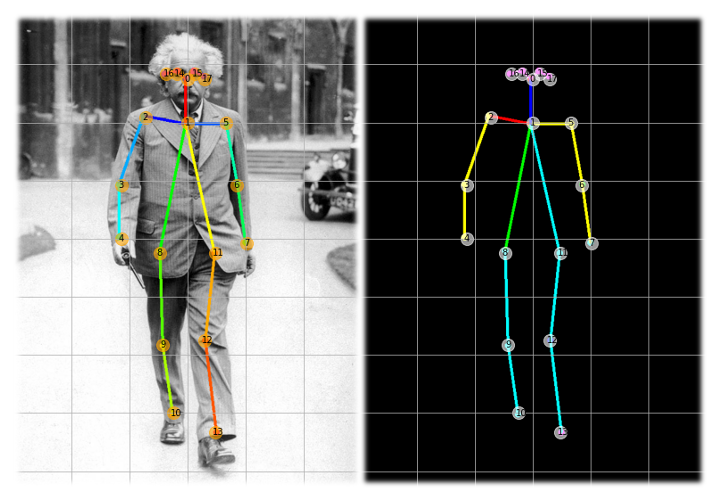
\includegraphics[scale=.5]{Figures/introduction-einstein.png}}
\caption{Example of human pose estimation key points \cite{rovai_realtime_2020}}
\label{example}
\end{figure}

A 3D point cloud is simply a set of points with three positional coordinates and represents points in 3D space. The points represent the shape of the object in 3D space. 3D point clouds are usually gathered by 3D scanners or dual-lens cameras.The output of scanners is point cloud where each point corresponds to some point on scanning surface with predefined precision. With the rapid growth of LIDAR and VR fields, the importance of accurate and fast 3D point cloud human pose estimation algorithms is clear.

\section{Challenges}
The obvious challenge of human pose estimation is the potential space of different human postures. The small change in the body part position changing the target pose. The task gets more complicated with different obstacles like clothes.
Using recent ML algorithms such as deep learning on 3D point cloud results in many challenges. Some of the common issues are:
\begin{itemize}
  \item The high dimensionality of the input space. Compared to pose estimation based on images, 3D point cloud has higher-dimensional space.
  \item Noisy inputs from 3D point cloud scanners. The sparsity and accuracy of the point cloud greatly influence the model's performance. The accuracy and granularity of points are significantly dependent on the scanning device. Compact LIDAR scanning devices the most popular and less accurate.
  \item Geometric-viewpoint relation. The human body has a strict geometric relation between body parts, which is invariant to the viewpoint. Most of the deep learning algorithms are not viewpoint agnostic resulting in additional challenges for human pose estimation.
  \item Lack of data. The amount of data for 3D point cloud human pose estimation is significantly less than regular image datasets. This fact is due to the high complexity of collecting 3D point cloud data, e.g., need special multicamera or LIDAR equipment, need diverse human positions, need different human constitutions.
\end{itemize}

\section{Motivation}
Human pose estimation is an important task that is used in different fields.
A recent class of deep learning architecture known as capsule networks \parencite{sabour_dynamic_2017} theoretically overcomes multiple conventional deep learning models for human pose estimation. Compared to CNNs, capsule networks, due to the dynamic routing algorithm, account for the spatial relation between the input scene parts. Additionally, capsule networks "learn" the object's geometric relationship and thus could be viewpoint agnostic \parencite{sabour_dynamic_2017}. These capsule networks' properties make them the right candidate for examining human pose estimators based on the point cloud.
Moreover, some experiments \parencite{wang_capsule_2020,gritsevskiy_capsule_2018} stated that capsule networks need less data for convergence compared to non-capsule models. Besides, due to latent space inside the capsule network, it is more noise agnostic than regular convolutional networks.

\section{Research Gap}
\begin{itemize}
  \item There is no capsule-based model for 3D human pose estimation task.
  \item There is no comparison of the influence of noisy data on capsule-based and non-capsule-based models for 3D space.
  \item There is no comparison of how well capsule-based works with limited dataset compared to regular models.
\end{itemize}

\section{Objective}
The work's objective is to propose a model based on a capsule network for a 3D point cloud human pose estimation. Evaluate the model on public benchmark dataset for human pose estimation. Compare results with state of the art approaches for the task as mentioned earlier. Evaluate the influence of the noise in training dataset on capsule-based and non-capsule-based networks. Measure the performance of the models with different sizes of training dataset.

\section{Paper structure}
Section \ref{Related work} covers the related work of human pose estimation based on both 2D images and 3D point clouds. This section described conventionally, and state of the art approaches for solving the issue. Reviews capsule networks for different 3D point cloud tasks like point classification, segmentation, and position estimation.

The rest of the paper is organized in the following manner:
\begin{itemize}
  \item Section \ref{Hypothesis} presents the project's hypothesis and problems;
    \item  section \ref{Dataset} describes the dataset which is used for training and evaluation along with evaluation metrics;
  \item  section \ref{Methodology} describes the approach for solving the project's objectives;
   \item  section \ref{Experiments} describes experiments on project's objections described in \ref{Methodology};
  \item  section \ref{Conclusions} sums up the paper's ideas and present brief conclusions and possible future work in this field.
\end{itemize}
\chapter{Related work}
\label{Related work}

In this chapter, we overview common approaches to solve problems with point clouds. We review common techniques, models, and algorithms for point clouds.

In Section~\ref{Deep learning approaches for point cloud} and Section~\ref{Point-based Methods} we review common approaches on how to use point clouds in deep learning, along with preprocessing methods for 3D point data.

In Section~\ref{Human pose estimation} we review models and techniques for the task of human pose estimation, both for 2D and 3D spaces.

In Section~\ref{Capsule network} we review the initial work on the capsule network which were released for the task of image classification. Also, we review few works which adapt capsule networks for 3D point cloud data.

\section{Deep learning approaches for point cloud}
\label{Deep learning approaches for point cloud}
The different number of points and high dimensionality of the point cloud input makes it challenging to use regular 2D convolutions. The typical approach for such an issue is the conversation of the point cloud to a different format. Such approaches are projection-based methods, volumetric-based methods, and other geometric-based methods.
\subsection{Projection-based methods} 
Projection-based methods take point cloud and project it into a different panel view. After the projection, each view provides a set of combined features for target classification, regression, or segmentation. The critical challenge for the projection-based algorithm is the multi-view feature aggregation into one global feature space.

MVCNN \parencite{su_multi-view_2015} is the first CNN-based architecture which recognize rendered views of different shapes independently from each other. The model's performance shows that even from one view the 3D shape could be recognized with competitive accuracy. Adding more views increase the overall accuracy of the model. The processing pipeline if the MVCNN is shown in Figure~\ref{img:mvcnn}.

\begin{figure}[htbp]
    \centerline{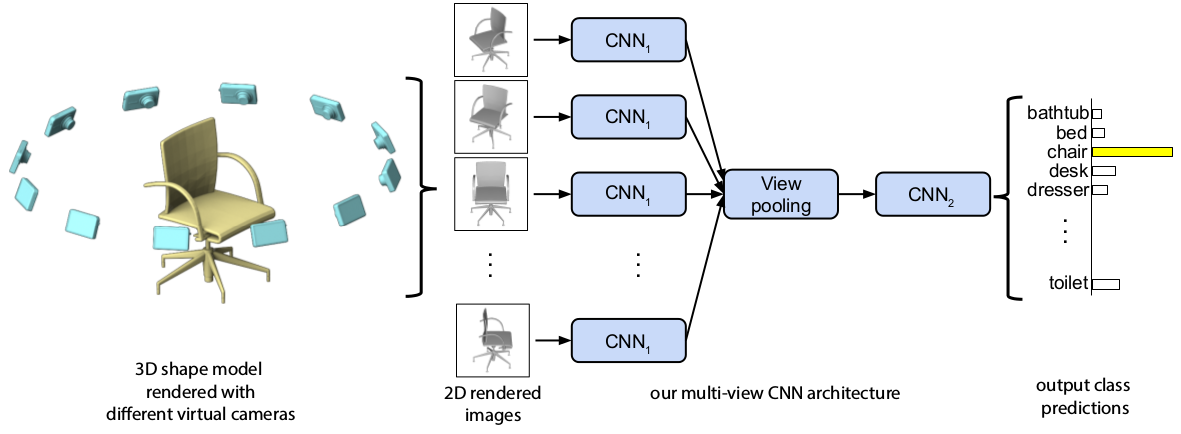
\includegraphics[scale=0.4]{Figures/mvcnn.png}}
    \caption{MVCNN processing pipeline  \parencite{su_multi-view_2015}}
    \label{img:mvcnn}
\end{figure}

MHBN \parencite{yu_multi-view_2018} (Multi-view Harmonized Bilinear Network) is the continuation of MVCNN. The approach proposes to integrates local convolutional features by harmonized bilinear pooling to produce a compact global descriptor.
To persist the information from different views, the View-GCN \parencite{wei_view-gcn_2020} proposes constructing view-graph with multiple views as graph nodes, then designing a graph convolutional neural network over view-graph to learn discriminative shape descriptor hierarchically.
All projection-based methods struggle from high memory consumption and high computational complexity since, for one feature extraction, the model should be run for the number of different views.

\subsection{Volumetric-based methods} 
Volumetric-based methods map the point cloud into a 3D grid. Then conventional 3D convolutions are using for feature extraction.
VoxNet \parencite{maturana_voxnet_2015} is the first method that exploits the volumetric representation of the point cloud. In this work, each cloud point is mapped to a discrete voxel point. The size of the target grid is 32 x 32 x 32 voxels. After the mapping, three convolutional layers are using to produce the target feature representations. Processing steps of VoxNet is shown in Figure~\ref{img:voxnet}

\begin{figure}[htbp]
    \centerline{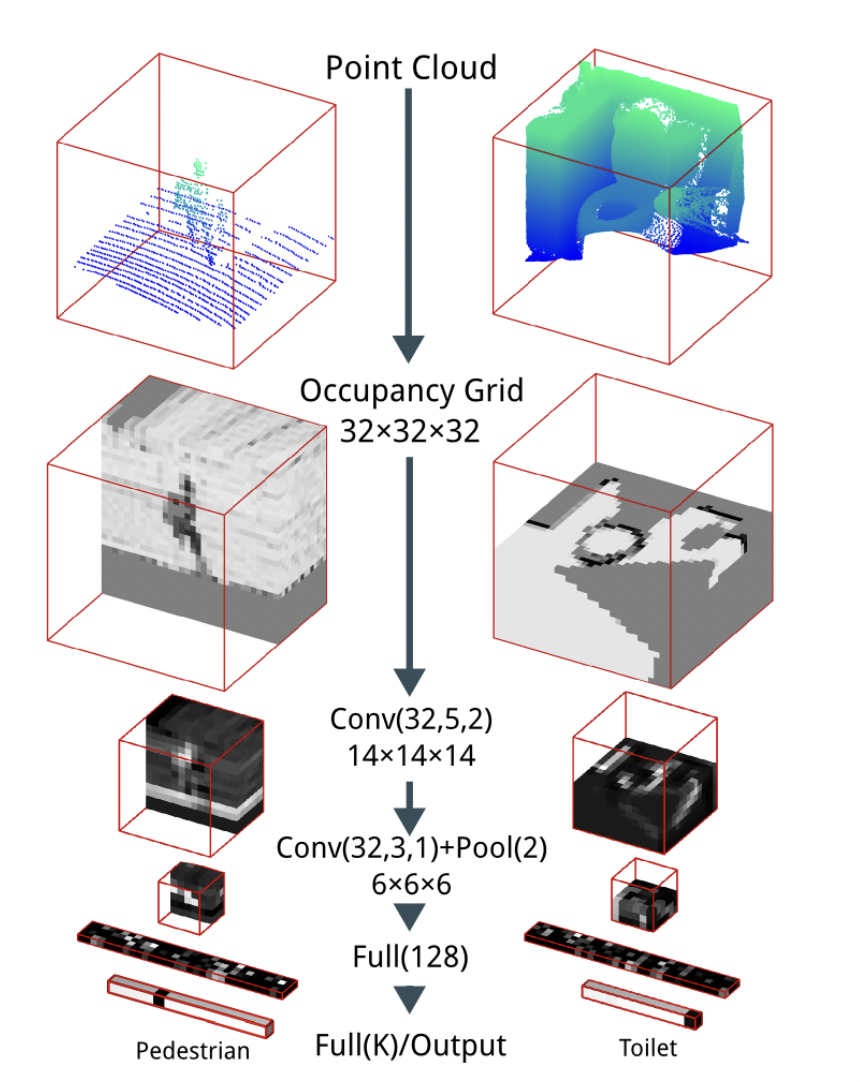
\includegraphics[scale=0.4]{Figures/VoxNet.png}}
    \caption{VoxNet processing pipeline  \parencite{maturana_voxnet_2015}}
    \label{img:voxnet}
\end{figure}

The more advanced volumetric-based models use octrees data structure. OctNet \parencite{riegler_octnet_2017} propose to represent the point cloud as several octrees along a regular grid (Figure~\ref{img:octTree}), each octree is encoded as a bit string, and features are generated through naive arithmetic. This approach reduces the memory consumption of the model during the training and inference stages.
The next iteration of octrees representation of point cloud is proposed in O-CNN \parencite{wang_o-cnn_2017}. The model uses 3D convolutions to extract features from octrees. This model also uses octree representation. The model takes the average normal vectors if 3D model from leafs of octants and runs 3D CNN on this to perform classification.

\begin{figure}[htbp]
    \centerline{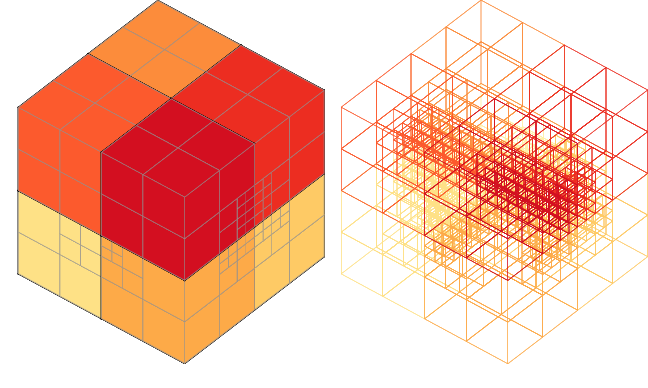
\includegraphics[scale=0.4]{Figures/OctNet.png}}
    \caption{An example of octree grid \parencite{riegler_octnet_2017}}
    \label{img:octTree}
\end{figure}


\section{Point-based Methods}
\label{Point-based Methods}
Compared with projection-based methods and volumetric-based methods that aggregate points from a spatial neighborhood, point-based methods attempt to learn features from individual points. Most of the recent work focuses on this direction.

The first work which uses a point-based approach is PointNet \parencite{qi_pointnet_2017}. PointNet learns pointwise features independently with several MLP layers and extracts global features with a max-pooling layer. The input (an $n \times 3$ 2D tensor) is first multiplied by an affine transformation matrix predicted by a mini-network (T-Net) to hold invariance under geometric transformations. The point set is then passed through a group of MLPs followed by another joint alignment network, and a max-pooling layer to obtain the final global feature. The model's architecture is depict in Figure~\ref{img:pointnet}

\begin{figure}[htbp]
    \centerline{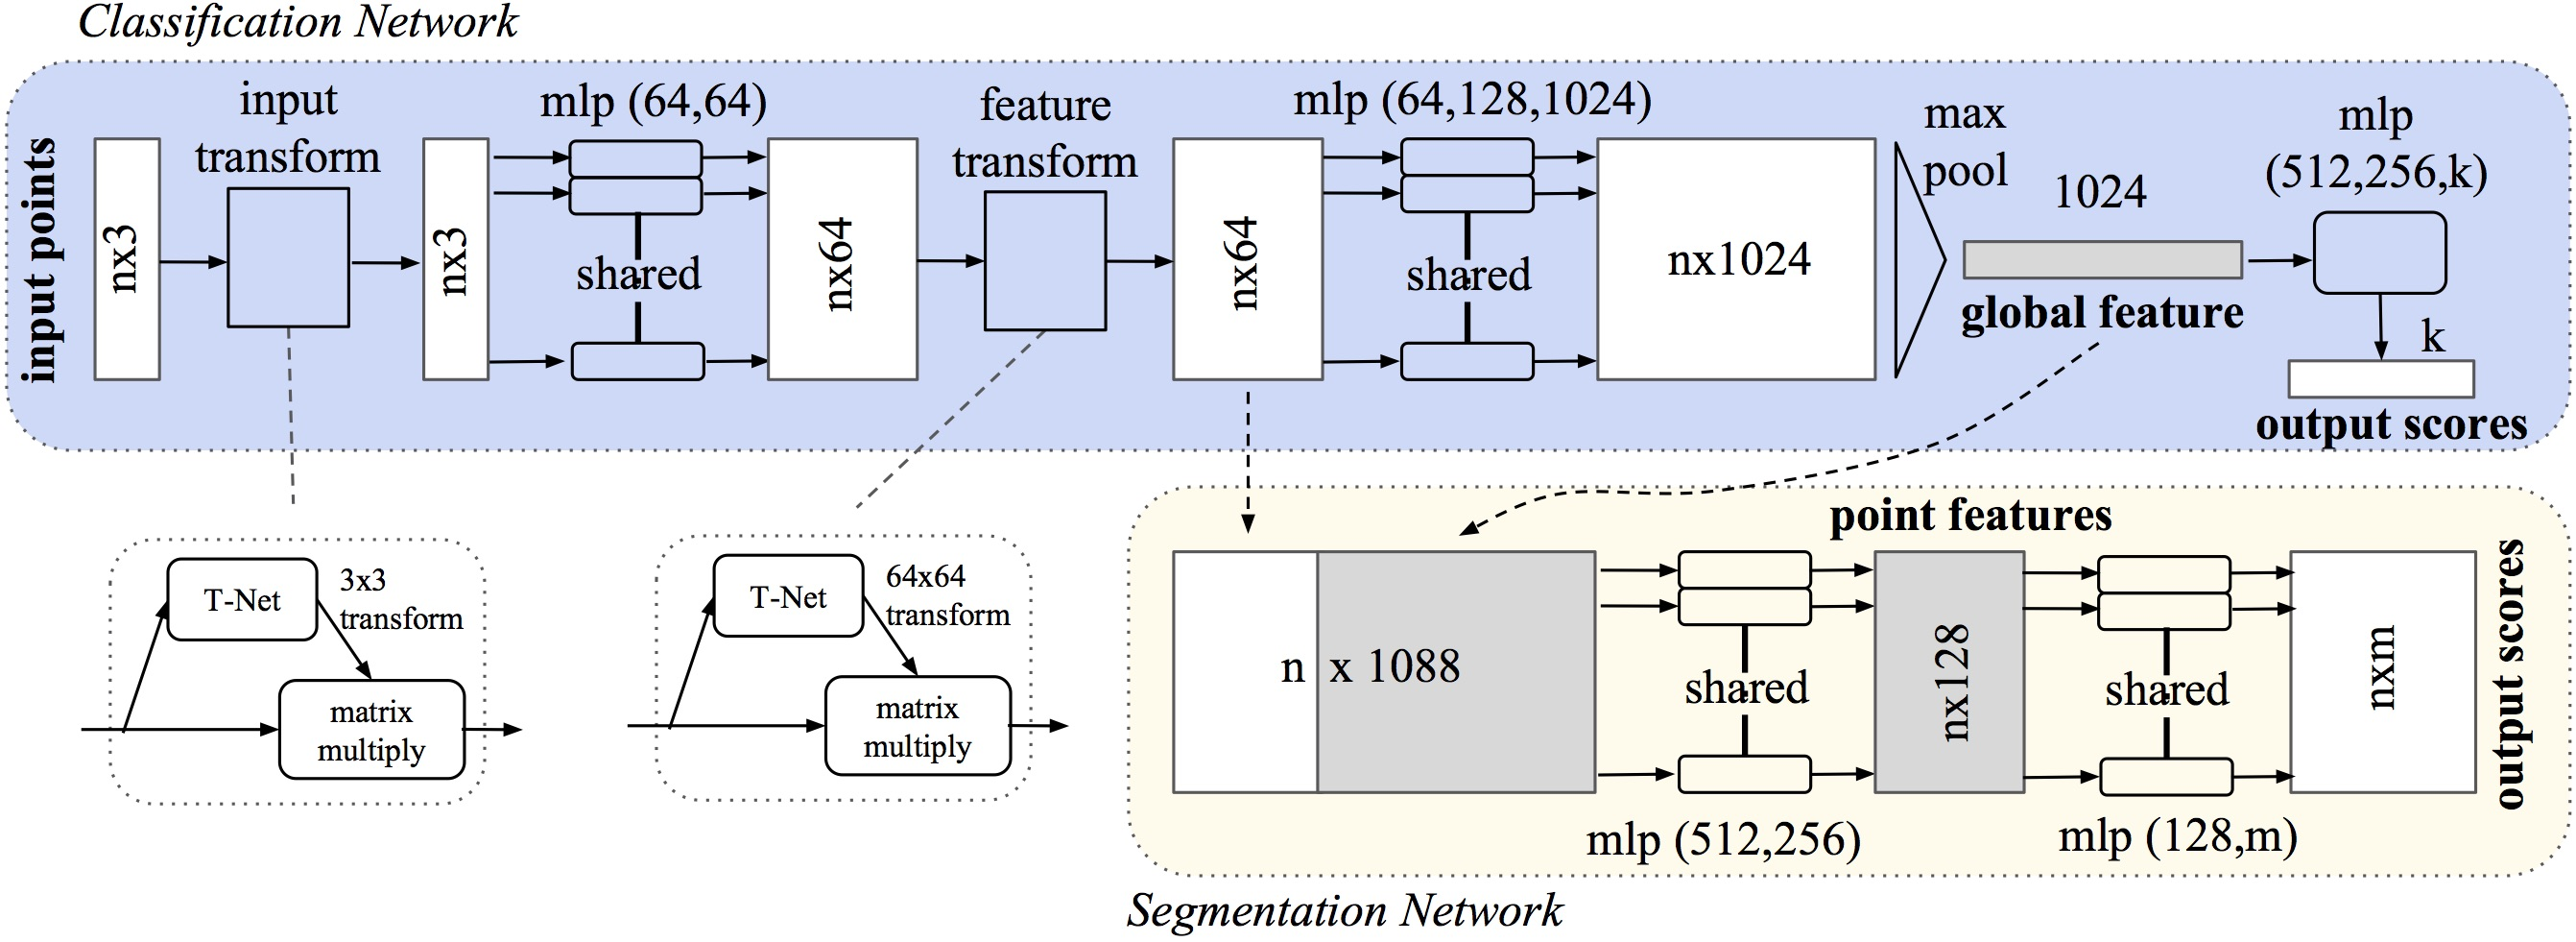
\includegraphics[scale=0.15]{Figures/pointnet.jpeg}}
    \caption{PointNet architecture \parencite{qi_pointnet_2017}}
    \label{img:pointnet}
\end{figure}

The second iteration of PointNet is PointNet++ \parencite{qi_pointnet_2017-1}. PointNet++ introduces a hierarchical neural network that applies PointNet recursively on a nested partitioning of the input point set. Using metric space distance, the model could learn local features with increasing contextual scale.
The state-of-the-art model for point-based classification is Point Attention Transformers \parencite{yang_modeling_2019}. The research for the first time proposes the mechanism of sampling which is end-to-end and task agnostic. The sampling is named "Gumbel Subset Sampling" - GSS. This sampling is used to select the most representative subset of the point cloud from the initial data. Using Gumble-Softmax, the model could provide a continuous point subset in the training phase, and a strict discrete subset in the test phase. Using such an approach the model is able to learn a more robust representation of the input data with less computational complexity.

\section{Human pose estimation}
\label{Human pose estimation}
The latest research approaches in the field of human pose estimation are based on deep learning.
There are two main approaches to the task:
\begin{itemize}
  \item pose estimation based on 2D images (mostly RGB);
  \item pose estimation based on the 3D point cloud.
\end{itemize}

The latter approach is more recent and promising. The 3D perspective gives more information for the models about body position in the space. Also, 3D point clouds mitigate the issue with occluded parts of the body. 2D image is a 2D projection of 3D space, and this transformation leads to the loss of information.

\subsection{Image-based methods}
The approaches for 2D image human pose estimation are divided into two types:
\begin{itemize}
  \item top-down approach
  \item bottom-up approach
\end{itemize}
In the top-down approach, the first step is person detection and then pose regression. In the bottom-up approach, all body parts are detected first and then grouped according to the body's position.

OpenPose \parencite{cao_openpose_2019} is the most popular example of bottom-up approaches for multi-person pose estimation. The network first extracts features from the image using the VGG feature extractor. Then features are passed to two separate branches, the first branch predicts body parts key points, the second branch predicts the associativity between body parts. The result of human pose estimation from OpenPose is shown in Figure~\ref{img:openpose}.

\begin{figure}[htbp]
    \centerline{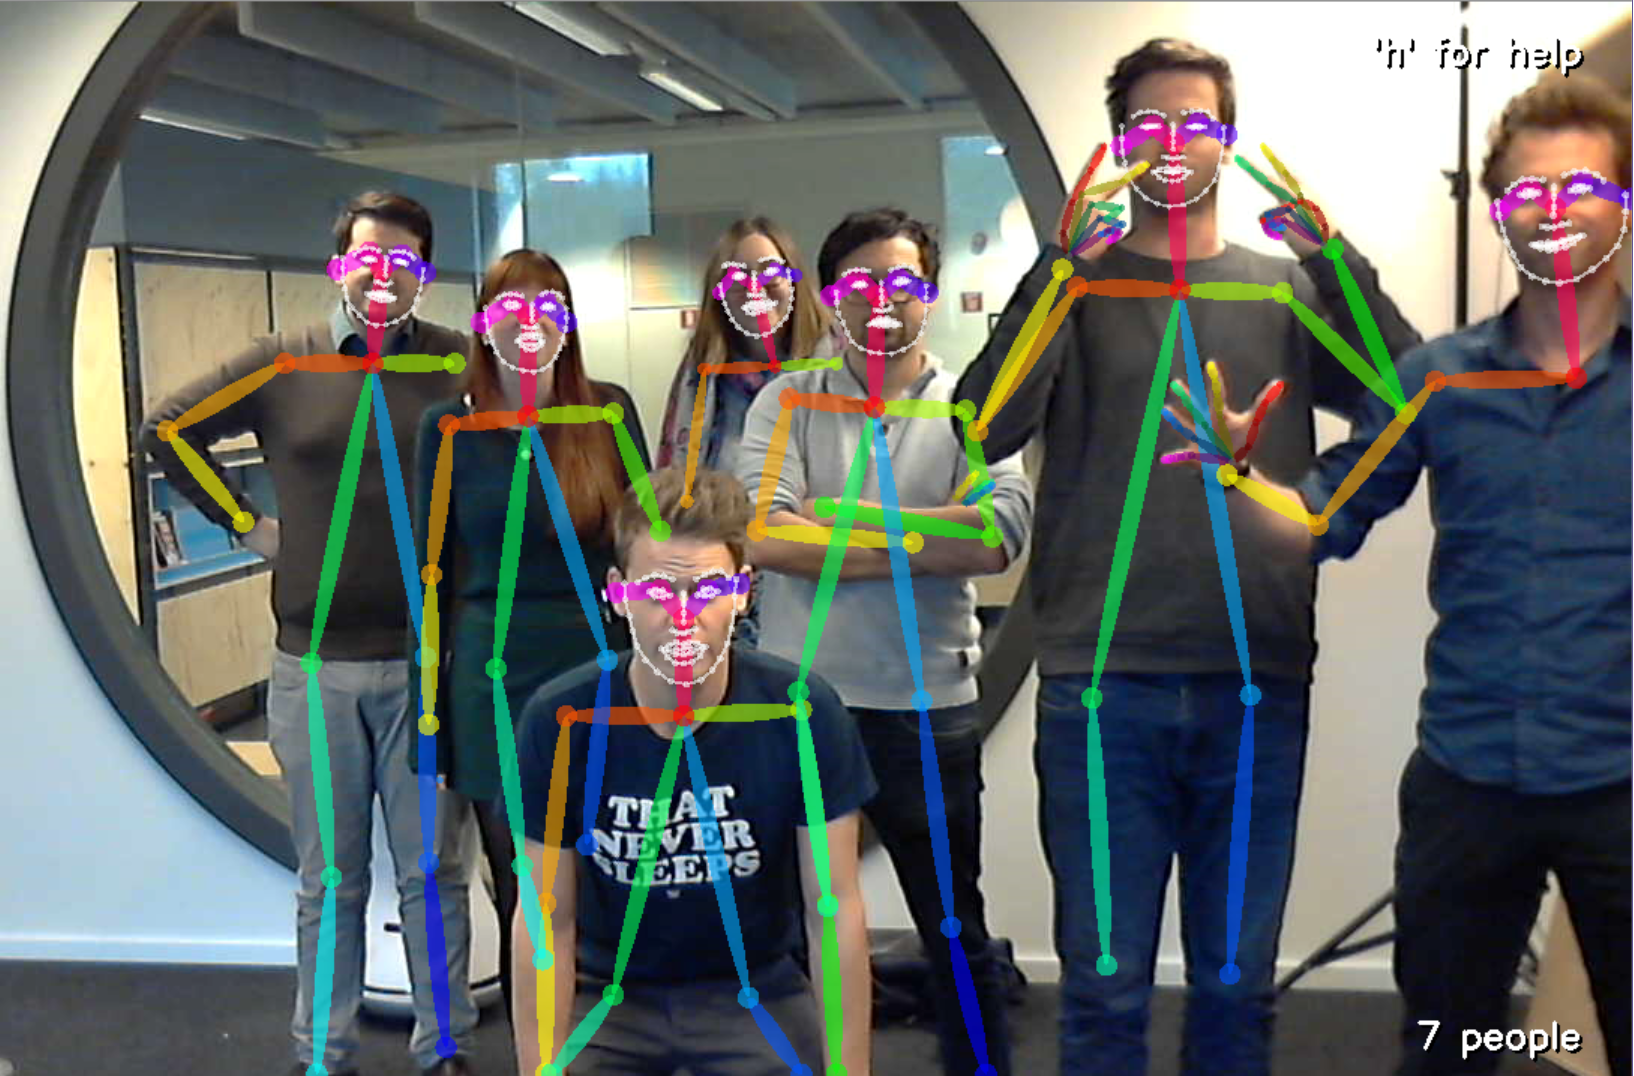
\includegraphics[scale=0.15]{Figures/OpenPose.png}}
    \caption{An example OpenPose network result  \parencite{cao_openpose_2019}}
    \label{img:openpose}
\end{figure}

RMPE (AlphaPose) \parencite{fang_rmpe_2018} is a top-down model.
This approach proposes to use a four-stage pipeline. The first step is Symmetric Spatial Transformer Network (SSTN). In this step, the model extracts the human region using a bounding box. The second step is a Single Person Pose Estimator (SPPE). This step model uses extracted human regions to estimate key joints of the human body. The third step is spatial De-Transformer Network (SDTN). This step remap estimated human joint coordinates back to the original coordinate system. The last step is parametric pose Non-Maximum Suppression (NMS). This step handles the issue with redundant pose deductions.

\subsection{point-cloud-based methods} 
Point cloud-based estimation is a relatively young field due to the recent growth of popularity of point cloud scanning devices.

The first model for human pose estimation based on point cloud was presented by \cite{diaz_barros_real-time_2015}. The paper presents an approach where based on a predefined human body skeleton the input point cloud is clustered using PCA and Expectation maximization algorithms.

The recent work in this field is presented by \cite{zhou_learning_2020}. The work takes point clouds as input data and model the surface of the object, in this research - human body, using deep human pose network. The pros of this approach is that it's an end-to-end model. It takes 2D depth image, transforms it to 3D point cloud, and then estimate key human joint coordinates. The model's architecture is shown in Figure~\ref{img:humreg}

\begin{figure}[htbp]
    \centerline{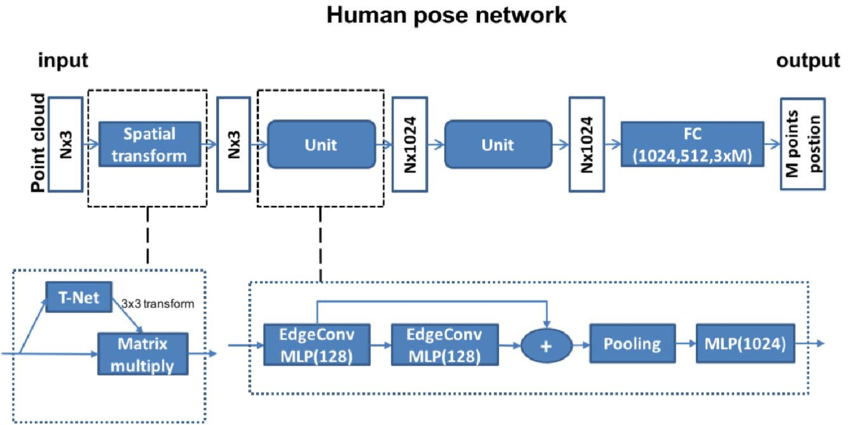
\includegraphics[scale=0.4]{Figures/human-regression-network.png}}
    \caption{Architecture of DNN presented by \parencite{zhou_learning_2020}}
    \label{img:humreg}
\end{figure}

More point cloud human pose estimation methods will be covered in the next subsection. The next subsection covers models which are based on capsule architecture.

\section{Capsule network}
\label{Capsule network}
The concept of the capsule was first proposed by Hinton \parencite{sabour_dynamic_2017} and has been widely used in 2D and 3D deep learning \parencite{kakillioglu_3d_2020, qin_detecting_2020, duarte_videocapsulenet_2018, lalonde_capsules_2018}.

Capsules are represented as a set of vectors. The length of the capsule's vector represents the probability of the object's presence. The direction of the vector describes the object's property e.g. position, viewpoint, size, shape, etc. For capsules' training Hinton proposes a new algorithm \parencite{sabour_dynamic_2017} called dynamic routing. The forward pass with dynamic routing propagates the input data from lower-level capsules to higher-level ones. Lower-level capsules pass learned and predicted data to the higher-level capsules. If multiple lower-level capsules agree (activated) then higher-level capsules activate accordingly. With each iteration of dynamic routing, each capsule gets more accurate.

\subsection{Capsule networks for point cloud classification}
The first work where capsule networks were applied to the problem of point cloud classification is 3DCapsNet \parencite{cheraghian_3dcapsule_2018}. In this work, a new capsule-based layer is proposed - ComposeCaps. ComposeCaps learns spatially relevant feature mapping that can be exploited for 3D point cloud classification. The architecture of the network is shown in Figure~\ref{img:3DCapsNet}

\begin{figure}[htbp]
    \centerline{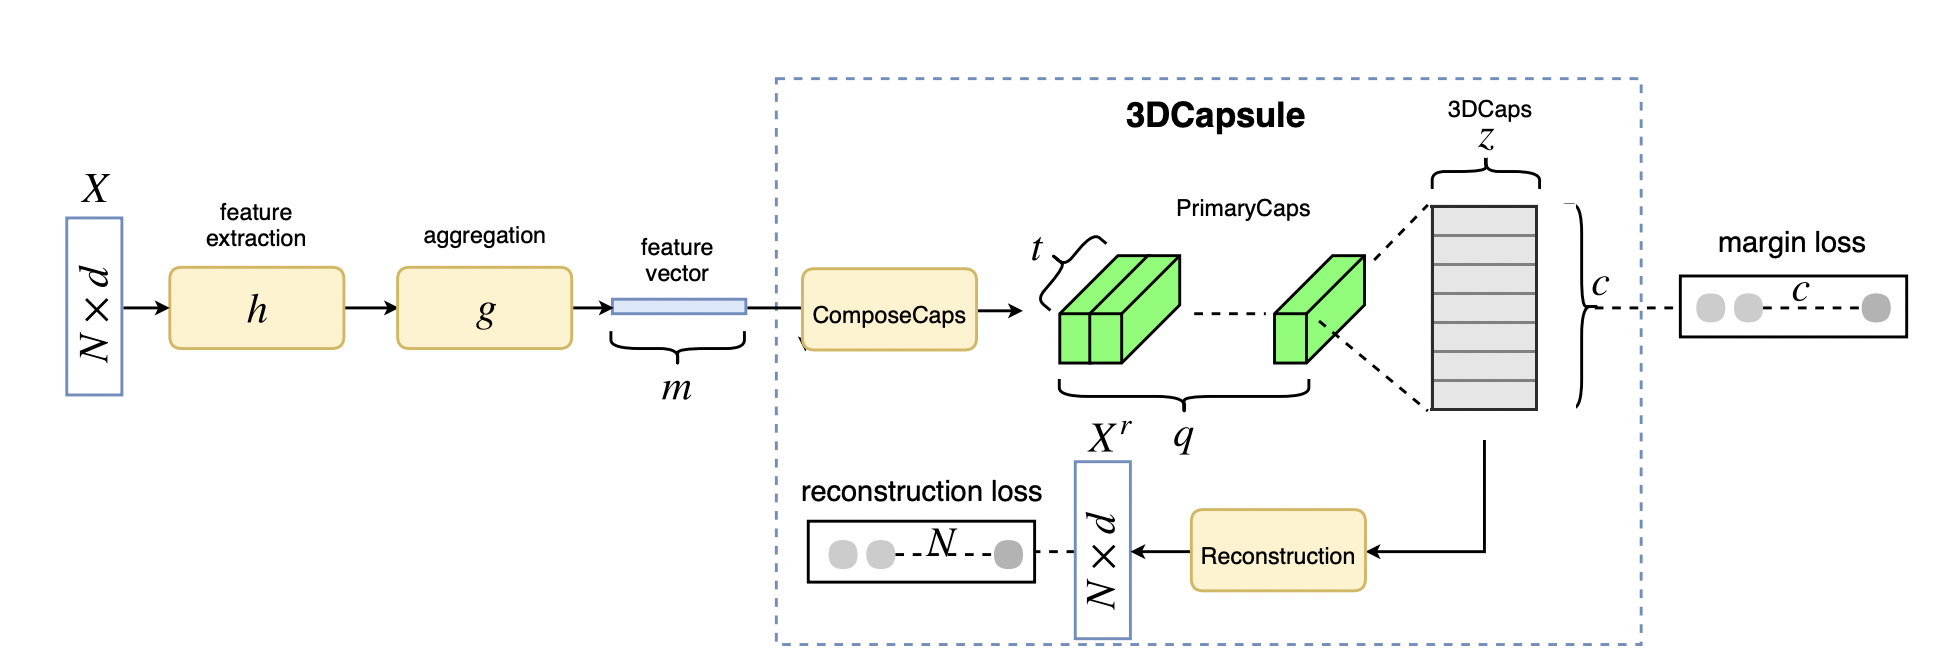
\includegraphics[scale=0.4]{Figures/3DCapsNet.png}}
    \caption{The architecture of 3DCapsNet \parencite{cheraghian_3dcapsule_2018}}
    \label{img:3DCapsNet}
\end{figure}

The second iteration of capsule applicability to 3D classification is the 3D point capsule network \parencite{zhao_3d_2019}. 3D point capsule network is an auto-encoder designed based on capsule networks. In this work researchers propose new architecture with a capsule network encoder that encodes input point cloud to capsules' latent space, and a decoder that decodes latent capsules. The proposed architecture works for several common point cloud-related tasks, such as object classification, object reconstruction, and part segmentation.

\subsection{Capsule networks for point cloud regression} 
The only work which is currently presented on the topic of point cloud regression is Capsule-HandsNet \parencite{wu_3d_2020}. This project is inspired by this research. Capsule-HandsNet uses model based on capsule auto-encoder proposed in \cite{zhao_3d_2019}. The model is an end-to-end, it takes hand point cloud and predicts key joints. The latent space of the model provides an ability to "memorize" the internal structures of the object such as symmetry, junction, relative location of object's parts, etc. The restored point cloud is combined from local patches predicted by capsules inside of the decoder (Figure~\ref{img:capshandnet}).   

\begin{figure}[htbp]
    \centerline{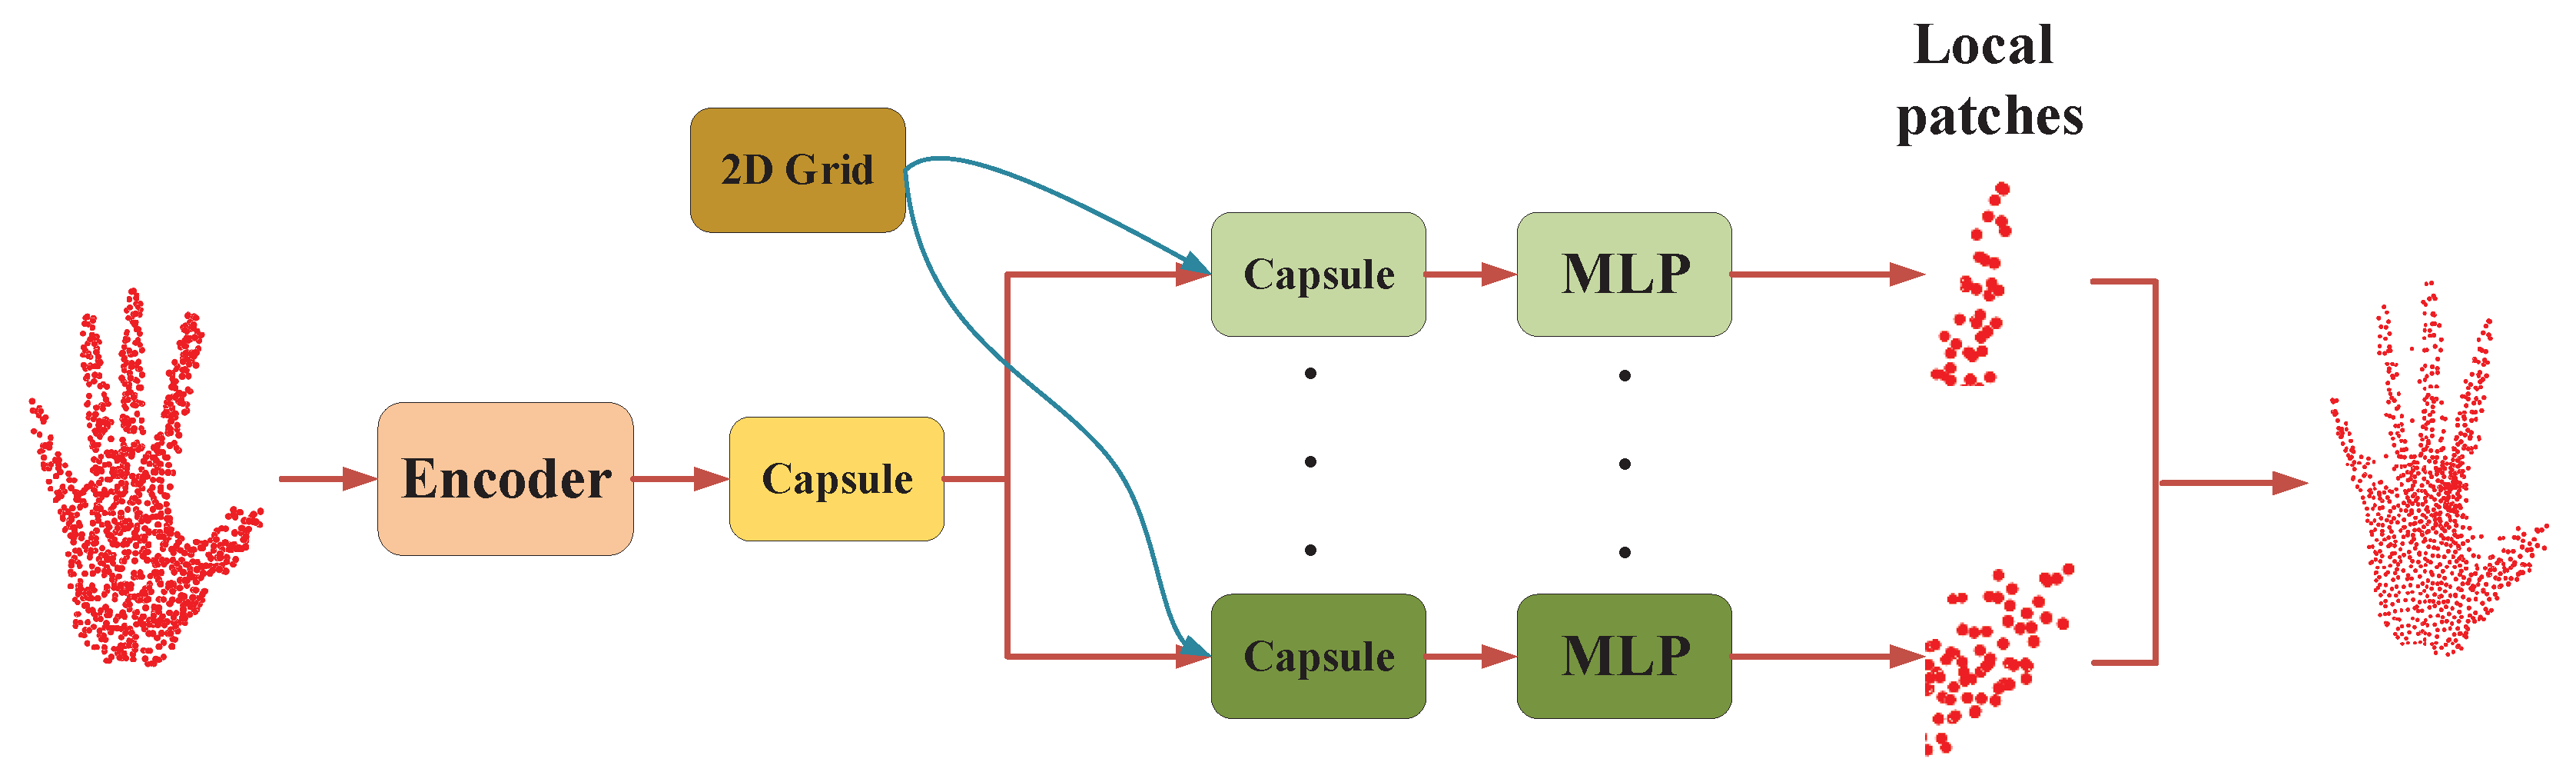
\includegraphics[scale=0.9]{Figures/caps-hand-net.png}}
    \caption{Reconstructed point cloud from capsule local patches \parencite{wu_3d_2020}}
    \label{img:capshandnet}
\end{figure}
 
\chapter{Research Hypothesis and Problem}

\label{Hypothesis}

\section{Hypotheses}
\paragraph{Model Comparison hypothesis:} This project's main objective is to create a model for human pose estimation based on point cloud using a capsule-based neural network, which shows competitive accuracy on well-known benchmarks.

\paragraph{Noise resistance hypothesis:} the impact of noise in the training dataset on the capsule-based model should be less compared to non-capsule models. Hypothesis is made based on 2D image recognition based using capsule networks \cite{sabour_dynamic_2017}.
Dataset size hypothesis: The dataset's size for full convergence should be smaller for capsule-based network compared to non-capsule ones. Assumption is made based on experiments presented in \cite{sabour_dynamic_2017} based on 2D image classification.

\section{Problems}
\paragraph{Noise problem.} To achieve the project goal mentioned above, we need to create an algorithm that could create realistic noise for point cloud data. We need to analyze and replicate factors that influence scanning devices' accuracy and result in noisy data.
\paragraph{Models' retrain problem.} To achieve the project's third goal, we need to retrain reference sota models with truncated training data. Hence, we need to allocate additional time for such an activity.
\chapter{Methodology}
\label{Methodology}

In this section we introduce the methodology for our proposed method for the task of human pose estimation using point cloud. As we reviewed in \ref{Related work} the key issue of any which use point clouds as an input is huge spatial variation of the data. Point clouds much diverse compared to 2D images in terms of location and rotation. Capsule networks shows promising results \parencite{sabour_dynamic_2017} on 2D data, and better handle spatial invariance compared to regular NN models.  \\
The chapter consists of two main section. In \ref{Data preparation} section we will cover the preprocessing for the input data and ground truths, and methods of adding artificial noise the the input data. In \ref{Network architecture} we will cover the network's architecture and algorithms for performing network's training.


\section{Data preparation}
\label{Data-preparation}
In this section we will cover main preprocessing steps for datasets. Preprocessing consists of:
\begin{enumerate}
  \item human extraction;
  \begin{enumerate}
    \item threshold filtering;
    \item clusterization \& cluster selection;
  \end{enumerate}
  \item point cloud normalization;
  \item adding noise to data (optional).
\end{enumerate}

On the first step we remove the most obvious points which doesn't represent human posture. On the second step we perform segmentation to extract "human" cluster. The third step is optional, and is used in experiments with performance of different models with various levels of the noise.  

On Figure~\ref{img:example-of-all-parts} are shown all steps of the preprocessing pipelines: threshold filtering, clusterization, and segmentation.

\begin{figure}[htbp]
    % \centerline{
    \hspace*{-1cm}                                                           
        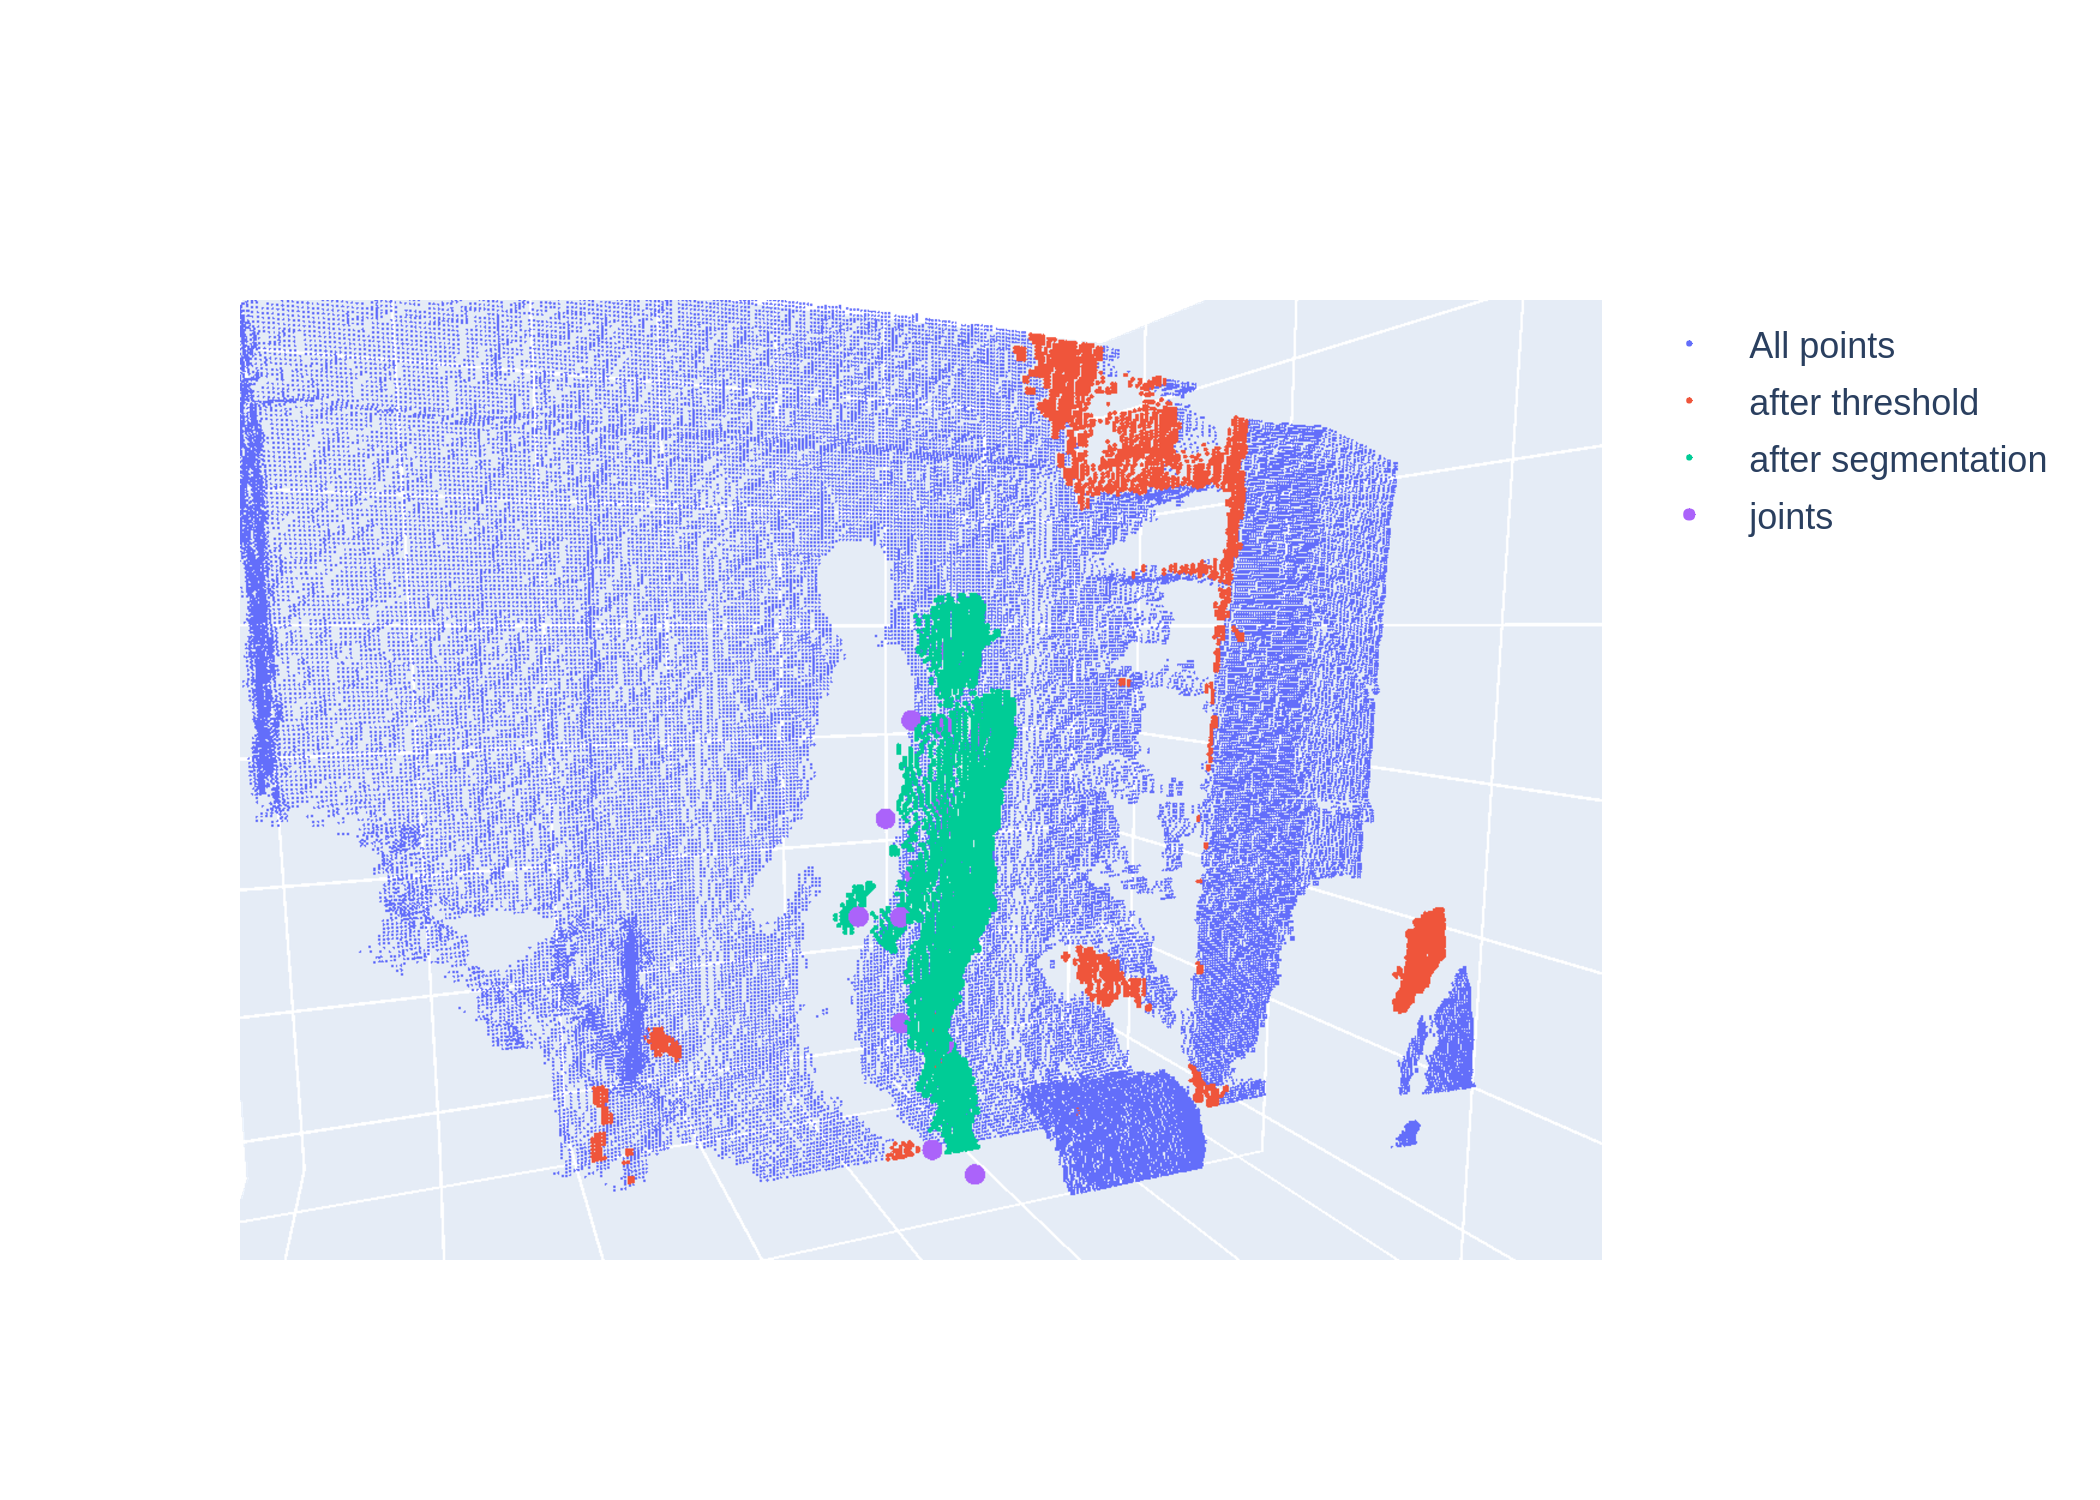
\includegraphics[trim=0 200 450 200,clip,scale=0.25]{Figures/example-all-parts.png}
    % }
    \caption{Example of preprocessing stages. \textbf{Blue} - points filtered by threshold. \textbf{Red} - points removed by human segmentation. \textbf{Green} - extracted human point cloud. \textbf{Purple} - key human joints}
    \label{img:example-of-all-parts}
\end{figure}

\subsection{Human extraction}
To start working with points cloud for human pose estimation we decided to extract human human points out of overall point cloud. As we can see from the Figure \ref{img:example-of-raw-data}, the raw point cloud contains not only human point cloud but also other objects which are located in the room, such as walls, cupboards, and other objects. These obstacles will not only harm the model's performance but will also greatly slow down the model's training and inference due to excess number of point.

\begin{figure}[htbp]
    \centerline{
        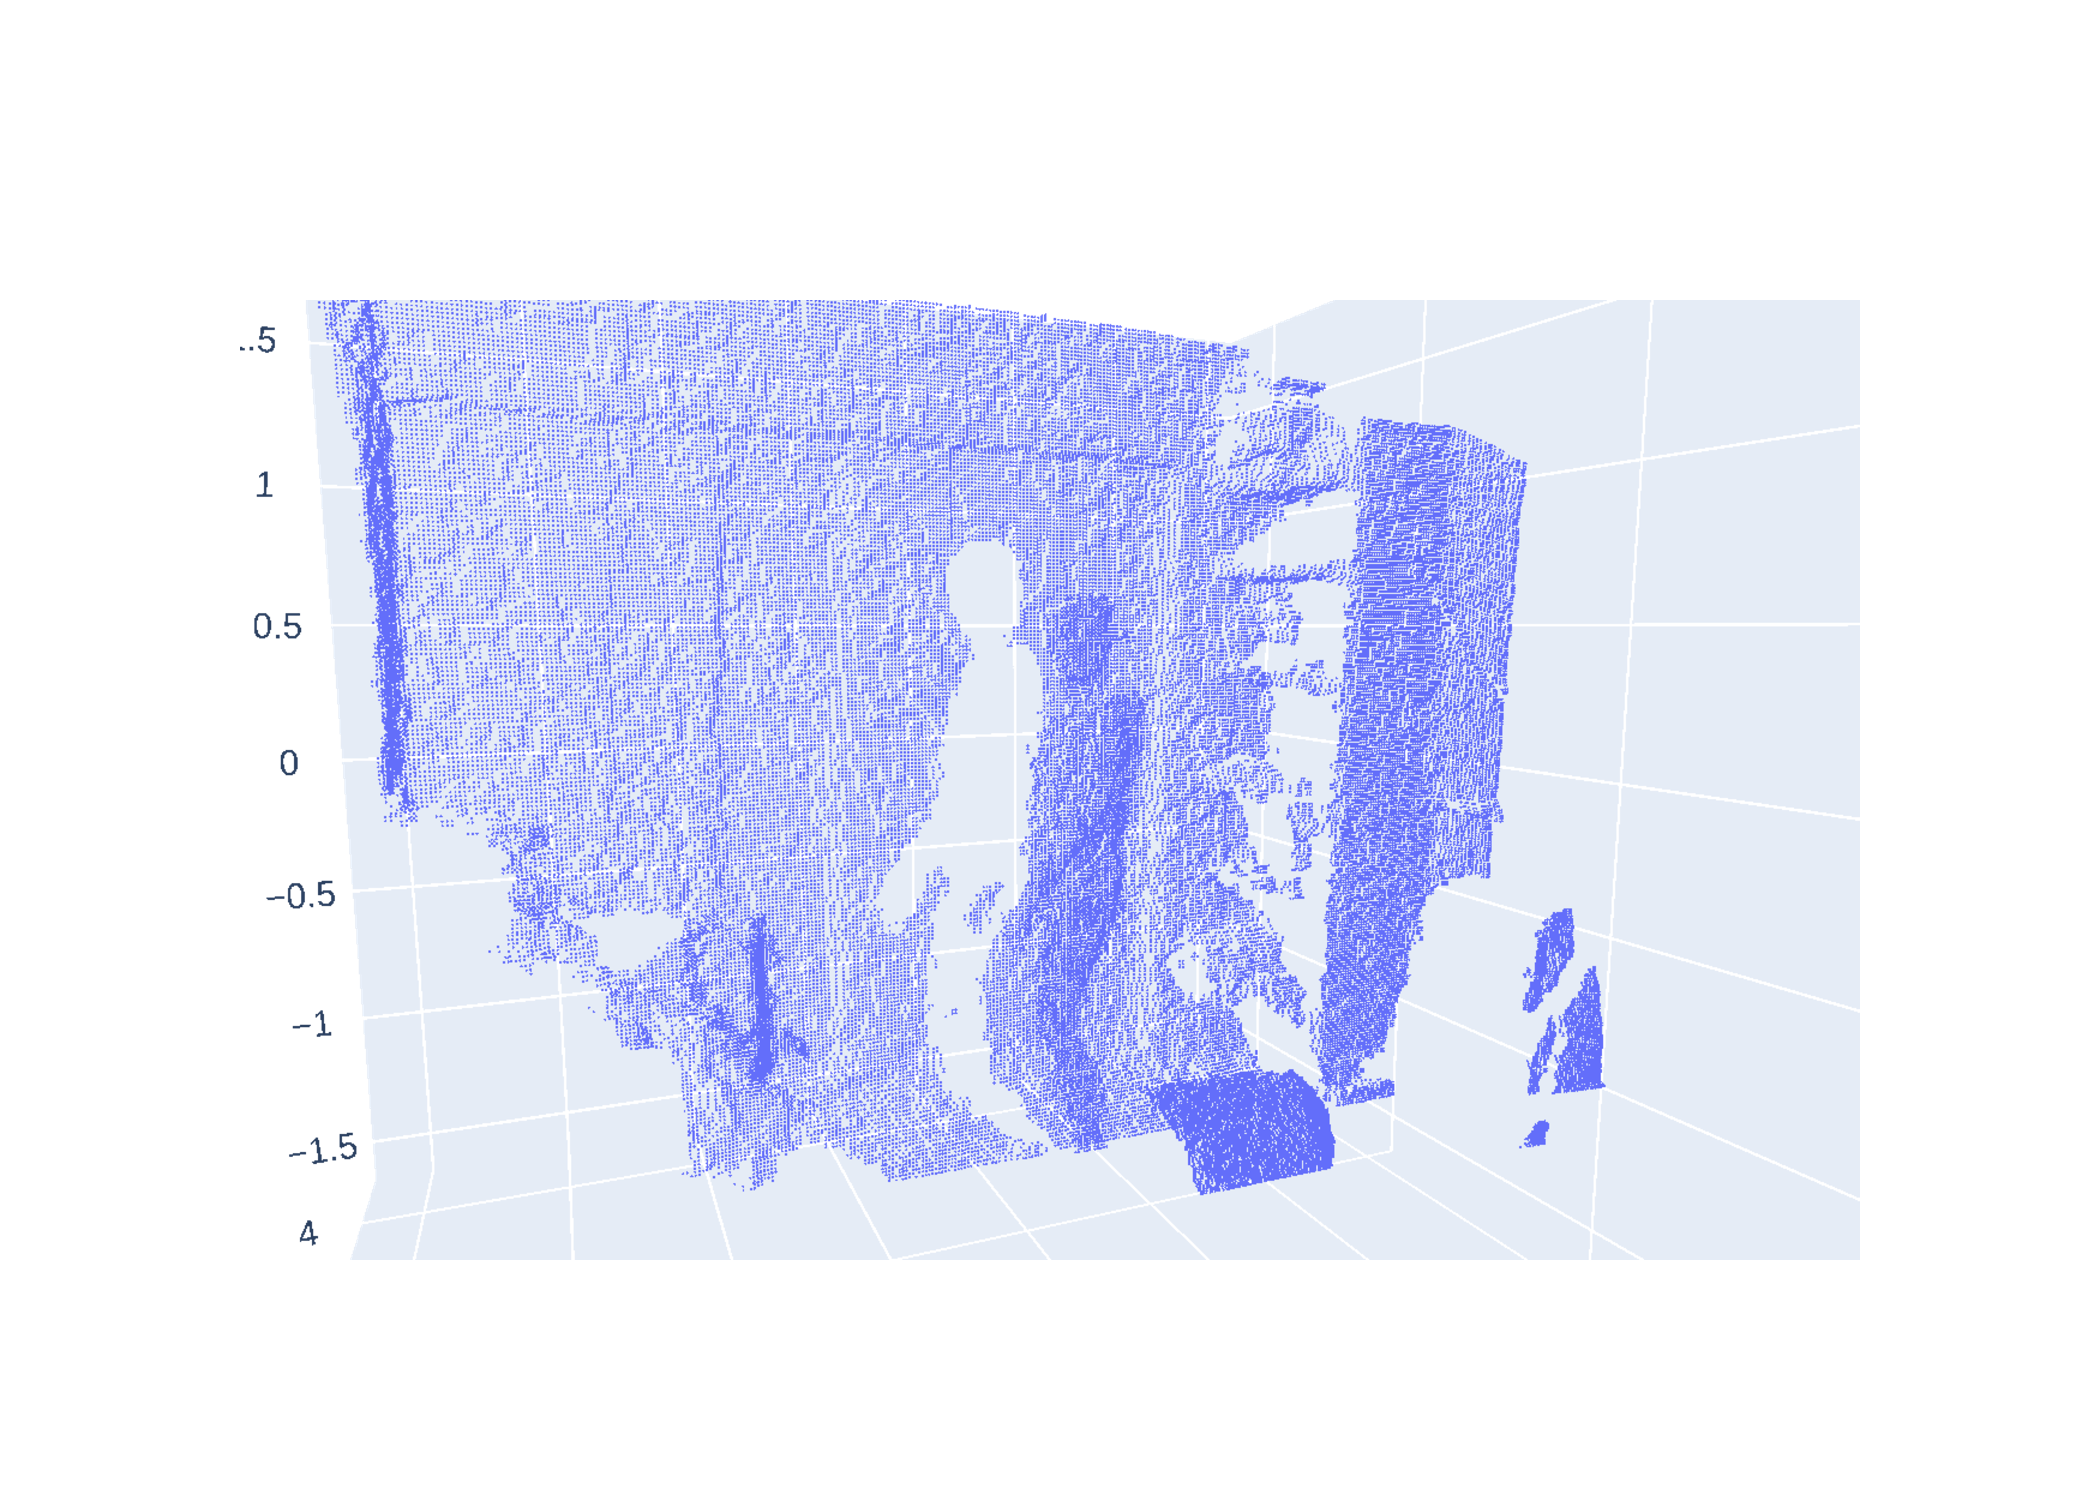
\includegraphics[trim=370 200 400 200,clip,scale=.25]{Figures/example-of-raw-data.png}
    }
    \caption{Example of raw data from ITOP dataset (front view)}
    \label{img:example-of-raw-data}
\end{figure}

\subsubsection{Threshold filtering}
\label{s:threshold-filtering}
Threshold filtering is the first step in preprocessing pipeline. The aim of this step is to filter out the most obvious points which don't belong to the human posture.
After manual checks we came up to such parameters:  

\begin{equation}
    \begin{aligned}
        x_{min} &= -1   &x_{max} &= 1 \\
        y_{min} &= -1.4 &y_{max} &= 2 \\
        z_{min} &= -1.5 &z_{max} &= 3.5
    \end{aligned}
\label{eqn:threshold-values}
\end{equation}

\ref{eqn:threshold-values} sets min-max distance values from camera view. The camera sensor is considered as center - $(0, 0, 0)$. In this way, $x$ coordinate represents left-right direction from the camera center, $y$ - top-bottom, and $z$ - the depth. \\
An example of threshold filtered point cloud could be seen in Figure~\ref{img:after-threshold-filtering}.

\begin{figure}[htbp]
    \centerline{
            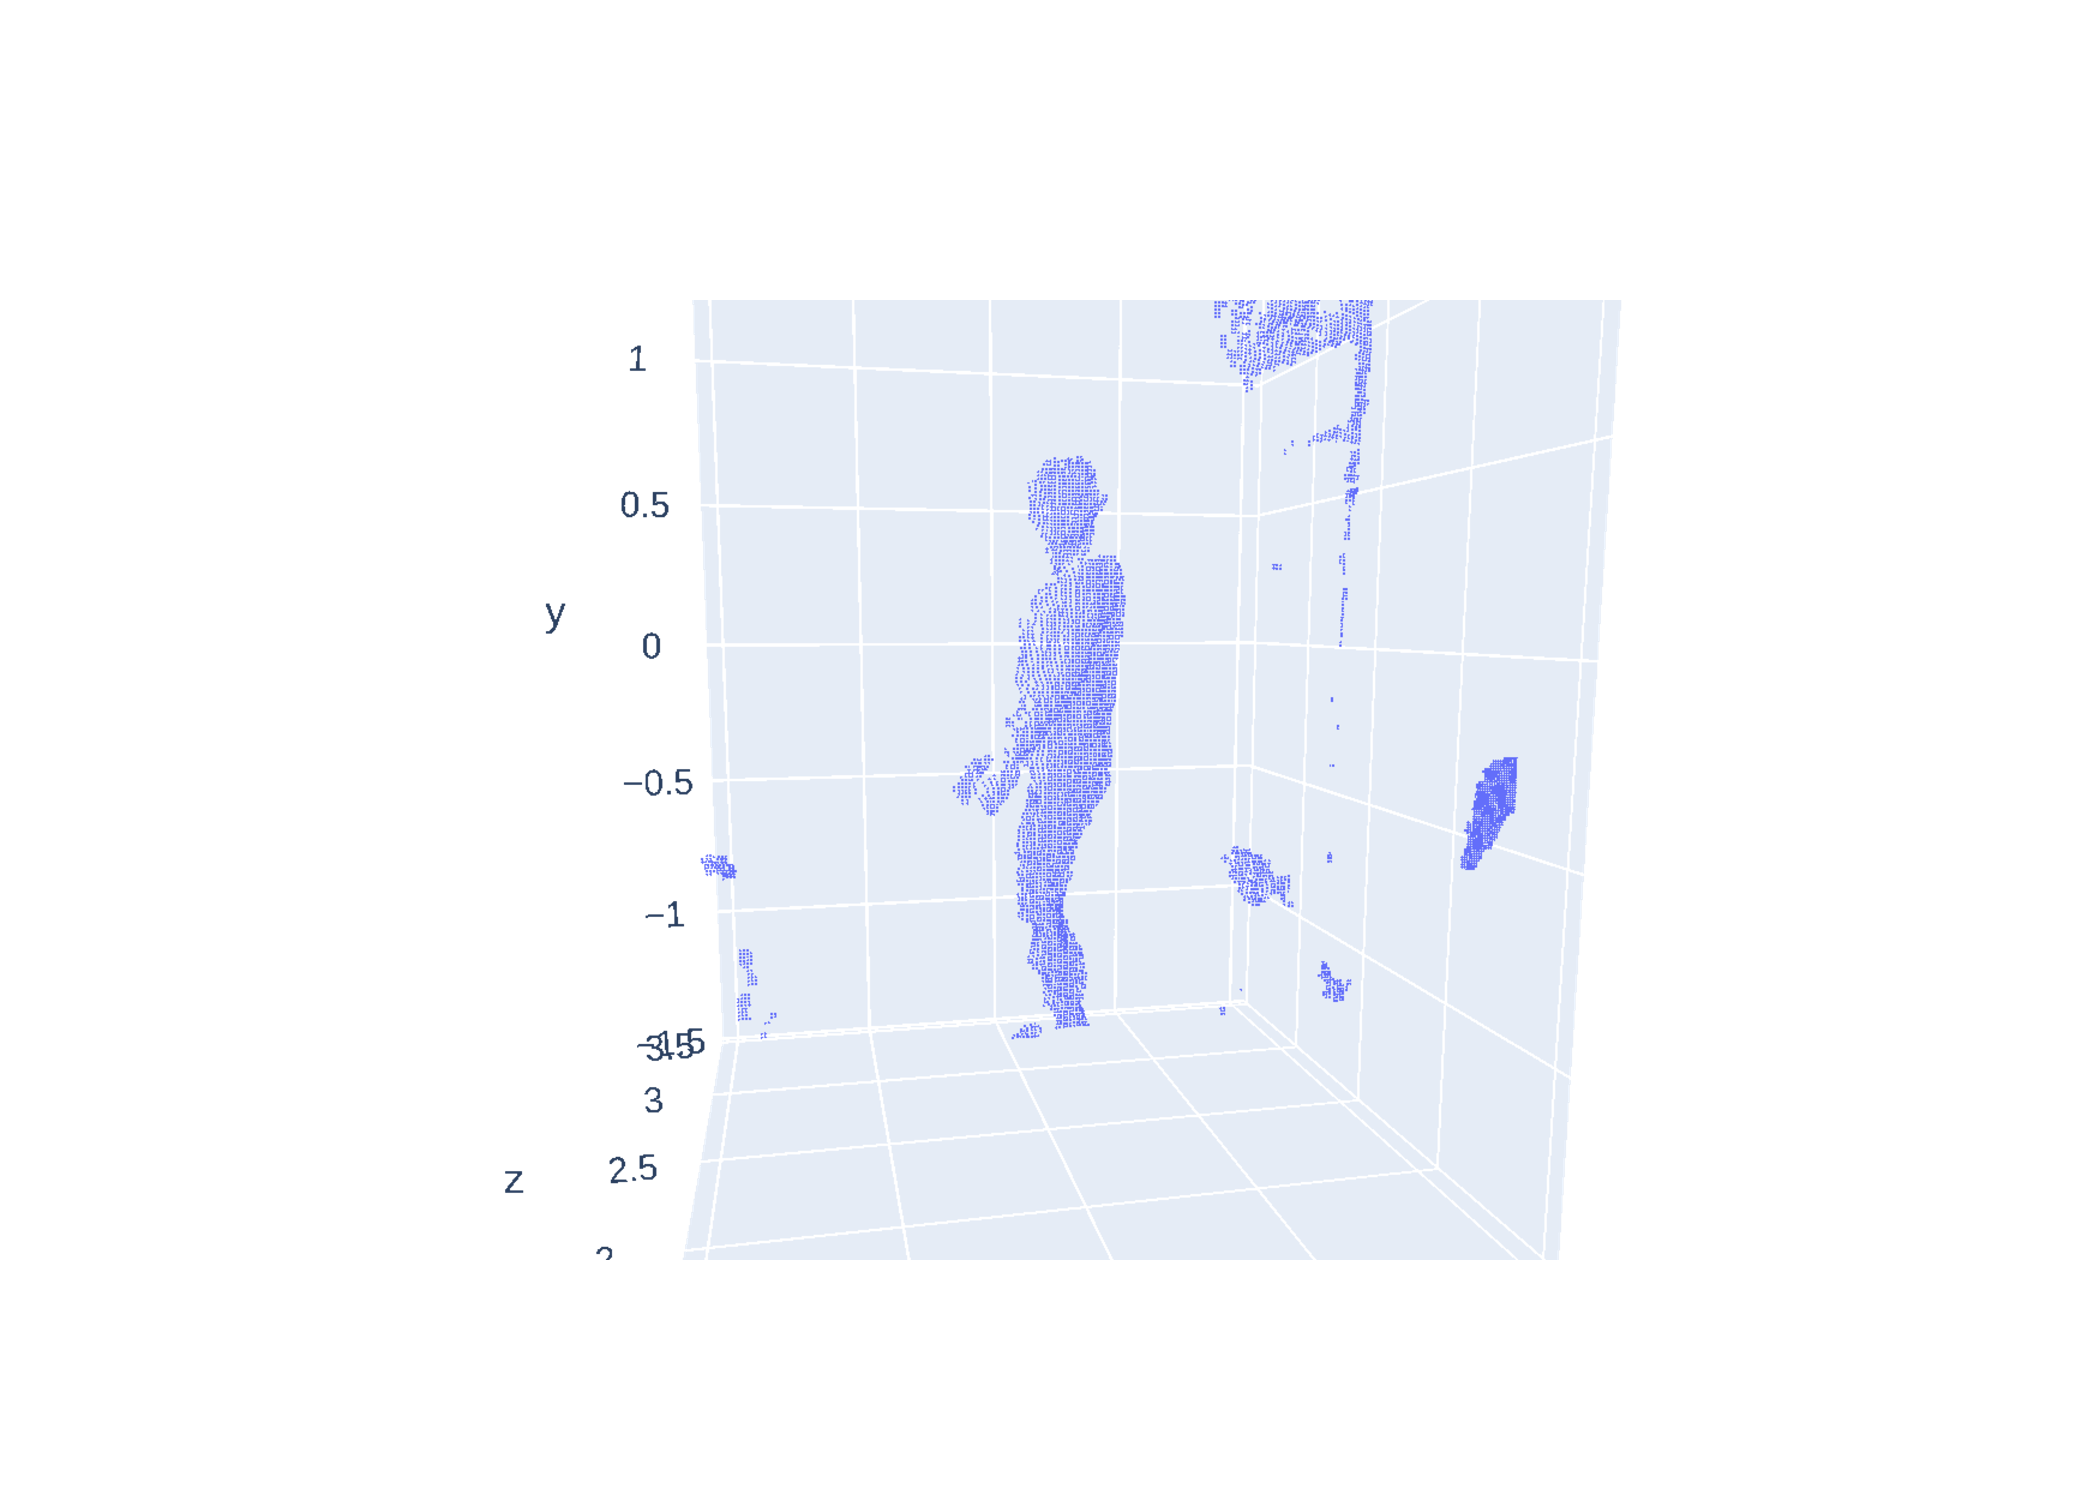
\includegraphics[trim=750 200 700 200,clip,scale=.35]{Figures/example-after-threshold.png}
    }
    \caption{Example of point cloud after applying of threshold filter}
    \label{img:after-threshold-filtering}
\end{figure}

\subsubsection{Clusterization}
The next step in preprocessing is clusterization \& extraction. On this step we clusterize point cloud from the \ref{s:threshold-filtering} and extract the human cluster. For clusterization step we propose the nearest-neighbour search algorithm \parencite{noauthor_nearest_2021} with kd-tree data-structure, using FLANN \footnote{Fast Library for Approximate Nearest Neighbor}. \\
The aim of the clusterization is separate human cluster and small noisy clusters from the point cloud. As we can see from the Algorithm~\ref{alg:clusterization}, for each point in initial point cloud $P$ we try to put it to some cluster based on the distance (radius - $r$) of that cluster. If the distance is less that radius to each cluster then this point creates a new cluster. At the end of clusterization we get a set of clusters $C$. \\
Since the human cluster always the biggest, at the end of clusterization we take the argmax and get human cluster $C_{human}$.

On the Figure~\ref{img:after-clustering} we can see the point cloud before clusterization, after, and the resulting human cluster (the biggest cluster). \\

\begin{algorithm}[H]
\label{alg:clusterization}
\SetAlgoLined
\KwResult{human point cloud cluster - $C_{human}$}
 create a Kd-tree representation for the input point cloud dataset $P$ \;
 set up an empty list of clusters $C$, and a queue of the points that need to be checked $Q$ \;
\For{\texttt{every point} $p_i \in P$} {
    add $p_i$ to the current queue $Q$ \;
    \For{\texttt{every point} $p_i \in Q$}{
        search for the set $P^k_i$ of point neighbors of $p_i$ in a sphere with radius $r < d_{th}$ \;
        for every neighbor $p^k_i \in P^k_i$, check if the point has already been processed, and if not add it to $Q$\;
    }
    when the list of all points in $Q$ has been processed, add $Q$ to the list of clusters $C$, and reset $Q$ to an empty list \;
}
the algorithm terminates when all points $\boldsymbol{p}_i \in P$ have been processed and are now part of the list of point clusters $C$ \;
$C_{human} = \underset{ x \in C }{\arg\max}$

\caption{Point cloud clusterization and human extraction \parencite{noauthor_pcl_nodate}}
\end{algorithm}

\begin{figure}[htbp]
    \centerline{
            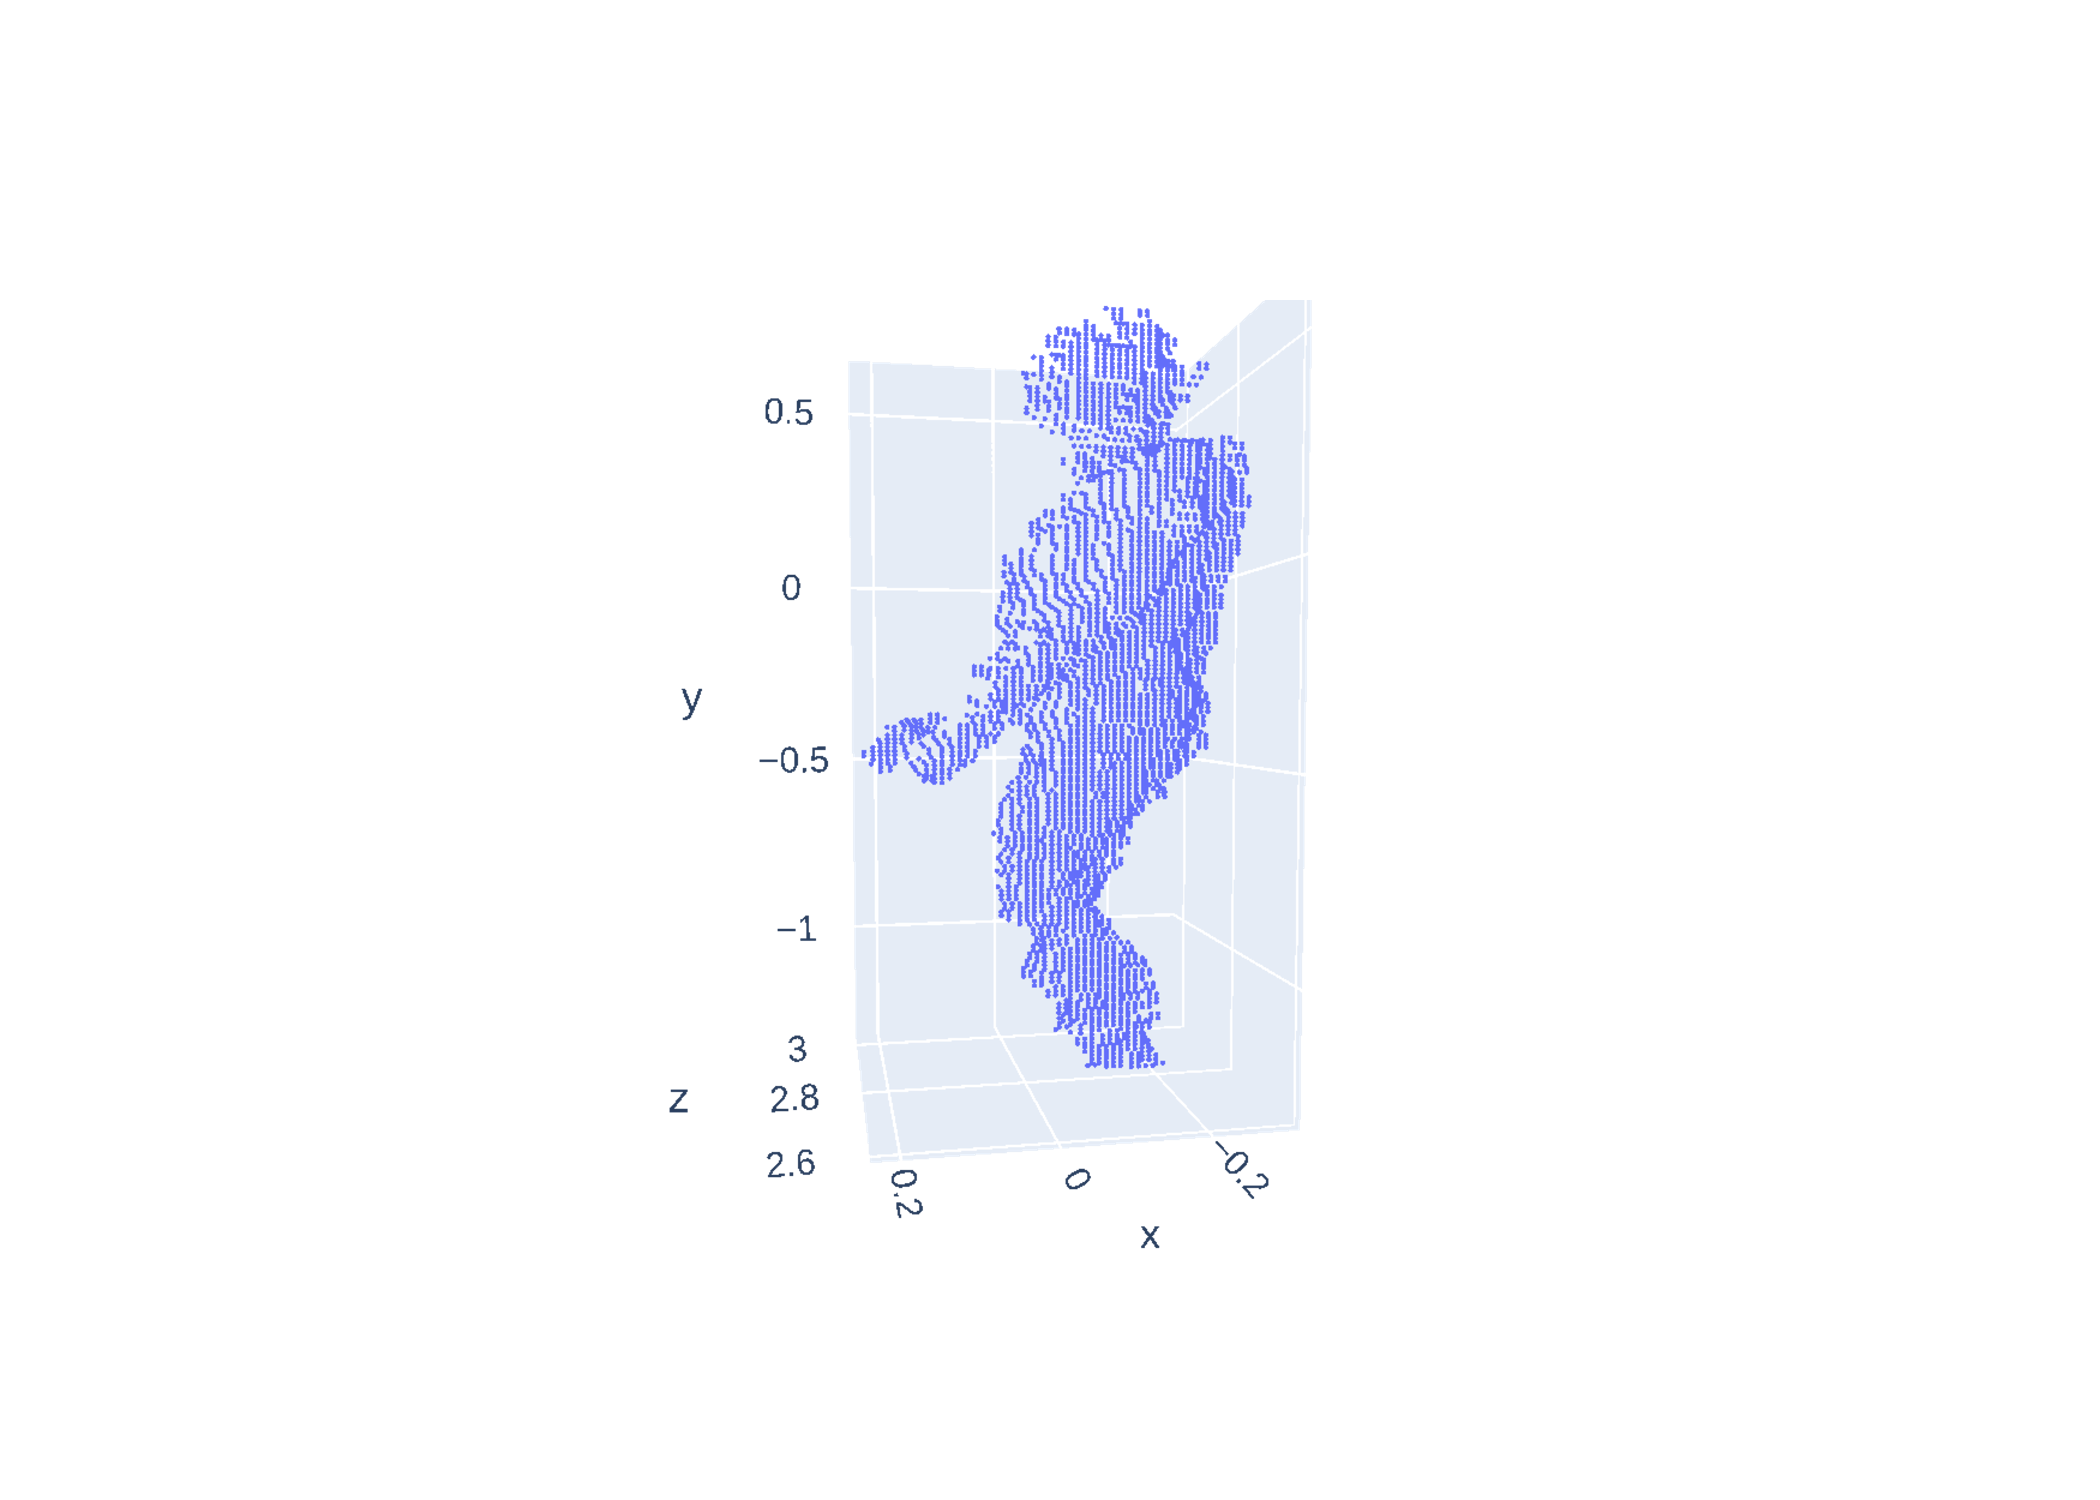
\includegraphics[trim=850 400 700 200,clip,scale=.3]{Figures/example-after-segmentation.png}
    }
    \caption{Example of point cloud after applying human extraction}
    \label{img:after-clustering}
\end{figure}

\subsection{Point cloud normalization}
TBD



\subsection{Adding noise to data}
Noise is the common thing in point cloud data. The origin the the noise could be environment conditions such as dust, fog, and other particles in the air. Also, the noise appears due to unperfectness on the lidar and other tools of creating point clouds.

In Experiment~\ref{s:experiment-noise} we investigate how models perform with different amount of artificial noise in the input data. For that we need to generate the noise which could be similar to the real-world. We propose to use two types of noise:
\begin{itemize}
  \item Gaussian noise;
  \item outlier noise.
\end{itemize}

\subsubsection{Gaussian noise}
The Gaussian noise is adding noise to the initial points in the point cloud $P$. With probability of $p$ the Gaussian noise ($\sigma$, $\mu$) is added to the point $p \in P$. In this way we simulate the unperfectness of the detecting device. The generation process is described in Algorithm~\ref{alg:gaussian-noise}

\begin{algorithm}[H]
\label{alg:gaussian-noise}
\SetAlgoLined
\KwResult{human point cloud with Gaussian noise  - $\hat{P_{human}}$}
\For{\texttt{every point} $p_i \in P$} {
    \If{ \texttt{uniRand()} < $Prob_{noise}$ } {
        Set $p_x$ to $p_x$ + $Gaus(\sigma, \mu)$ \;
        Set $p_y$ to $p_y$ + $Gaus(\sigma, \mu)$ \;
        Set $p_z$ to $p_z$ + $Gaus(\sigma, \mu)$ \;
    }
}
\caption{Adding Gaussian noise to point cloud \parencite{uchida_tom-uchidaadd_noise_to_point_cloud_2021}}
\end{algorithm}

An example of applying the Gaussian noise to the point cloud could be seen in the Figure~\ref{img:gaussian-noise}

\begin{figure}[htbp]
    \centerline{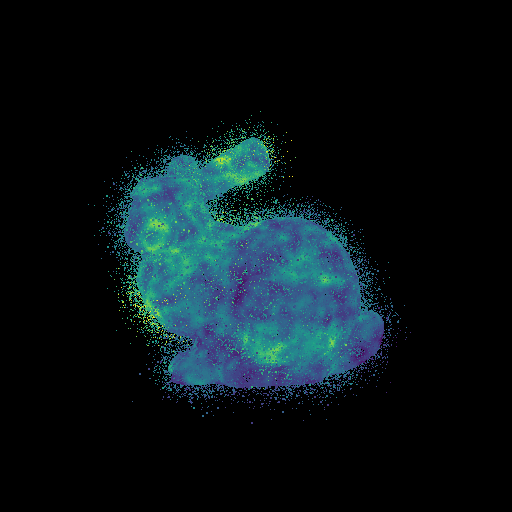
\includegraphics[scale=.6]{Figures/coords_gaussian.png}}
    \caption{Example of pllying the Gaussian noise to the point cloud \parencite{uchida_tom-uchidaadd_noise_to_point_cloud_2021}}
    \label{img:gaussian-noise}
\end{figure}

\subsubsection{Outlier noise}
The outlier noise adding new points to the initial point cloud $P$. The amount of outlier noise is defined by the fraction of the noise points compared to the initial number of human points. The noise point is taken from the uniform distribution $U(a, b)$. Where $a$ and $b$ are min-max values from the initial point cloud. In this way, outlier noise will fill uniformly the bounding box of the initial point cloud.

An example of addition of the outlier noise to the point cloud could be seen in the Figure~\ref{img:outlier-noise}

\begin{figure}[htbp]
    \centerline{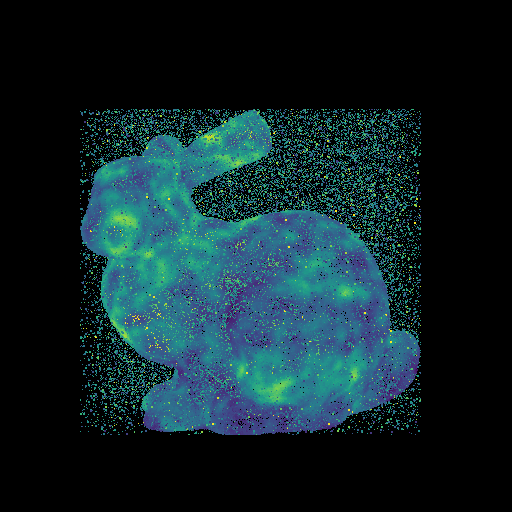
\includegraphics[scale=.6]{Figures/coords_outlier.png}}
    \caption{Example of addition the outlier noise to the point cloud \parencite{uchida_tom-uchidaadd_noise_to_point_cloud_2021}}
    \label{img:outlier-noise}
\end{figure}

\section{Network architecture}
\label{Network architecture}

In this section we will cover the network architecture for the task of human pose estimation, the loss functions, and the process of training.
As a <<<backbone>>> the work of \cite{wu_3d_2020} was used.


We designed a network based on the work of \cite{wu_3d_2020} to estimate the human pose. In this work we perform one-shot training strategy compared to the previous two-sage approaches. The aforementioned work perform two-stage training. The first stage consists of training of autoecoder part of the network to recreate the input human point cloud. Second stage takes autoencoder with freezed layers from the first stage and training a regression part of the modes which uses capsule outputs as input data. Such approach requires two steps in training pipeline and increase the number of huperparameter to tune the network. In this work we propose one-shot training scheme which is described in Section~\ref{network-training}.

\begin{figure}[htbp]
    \centerline{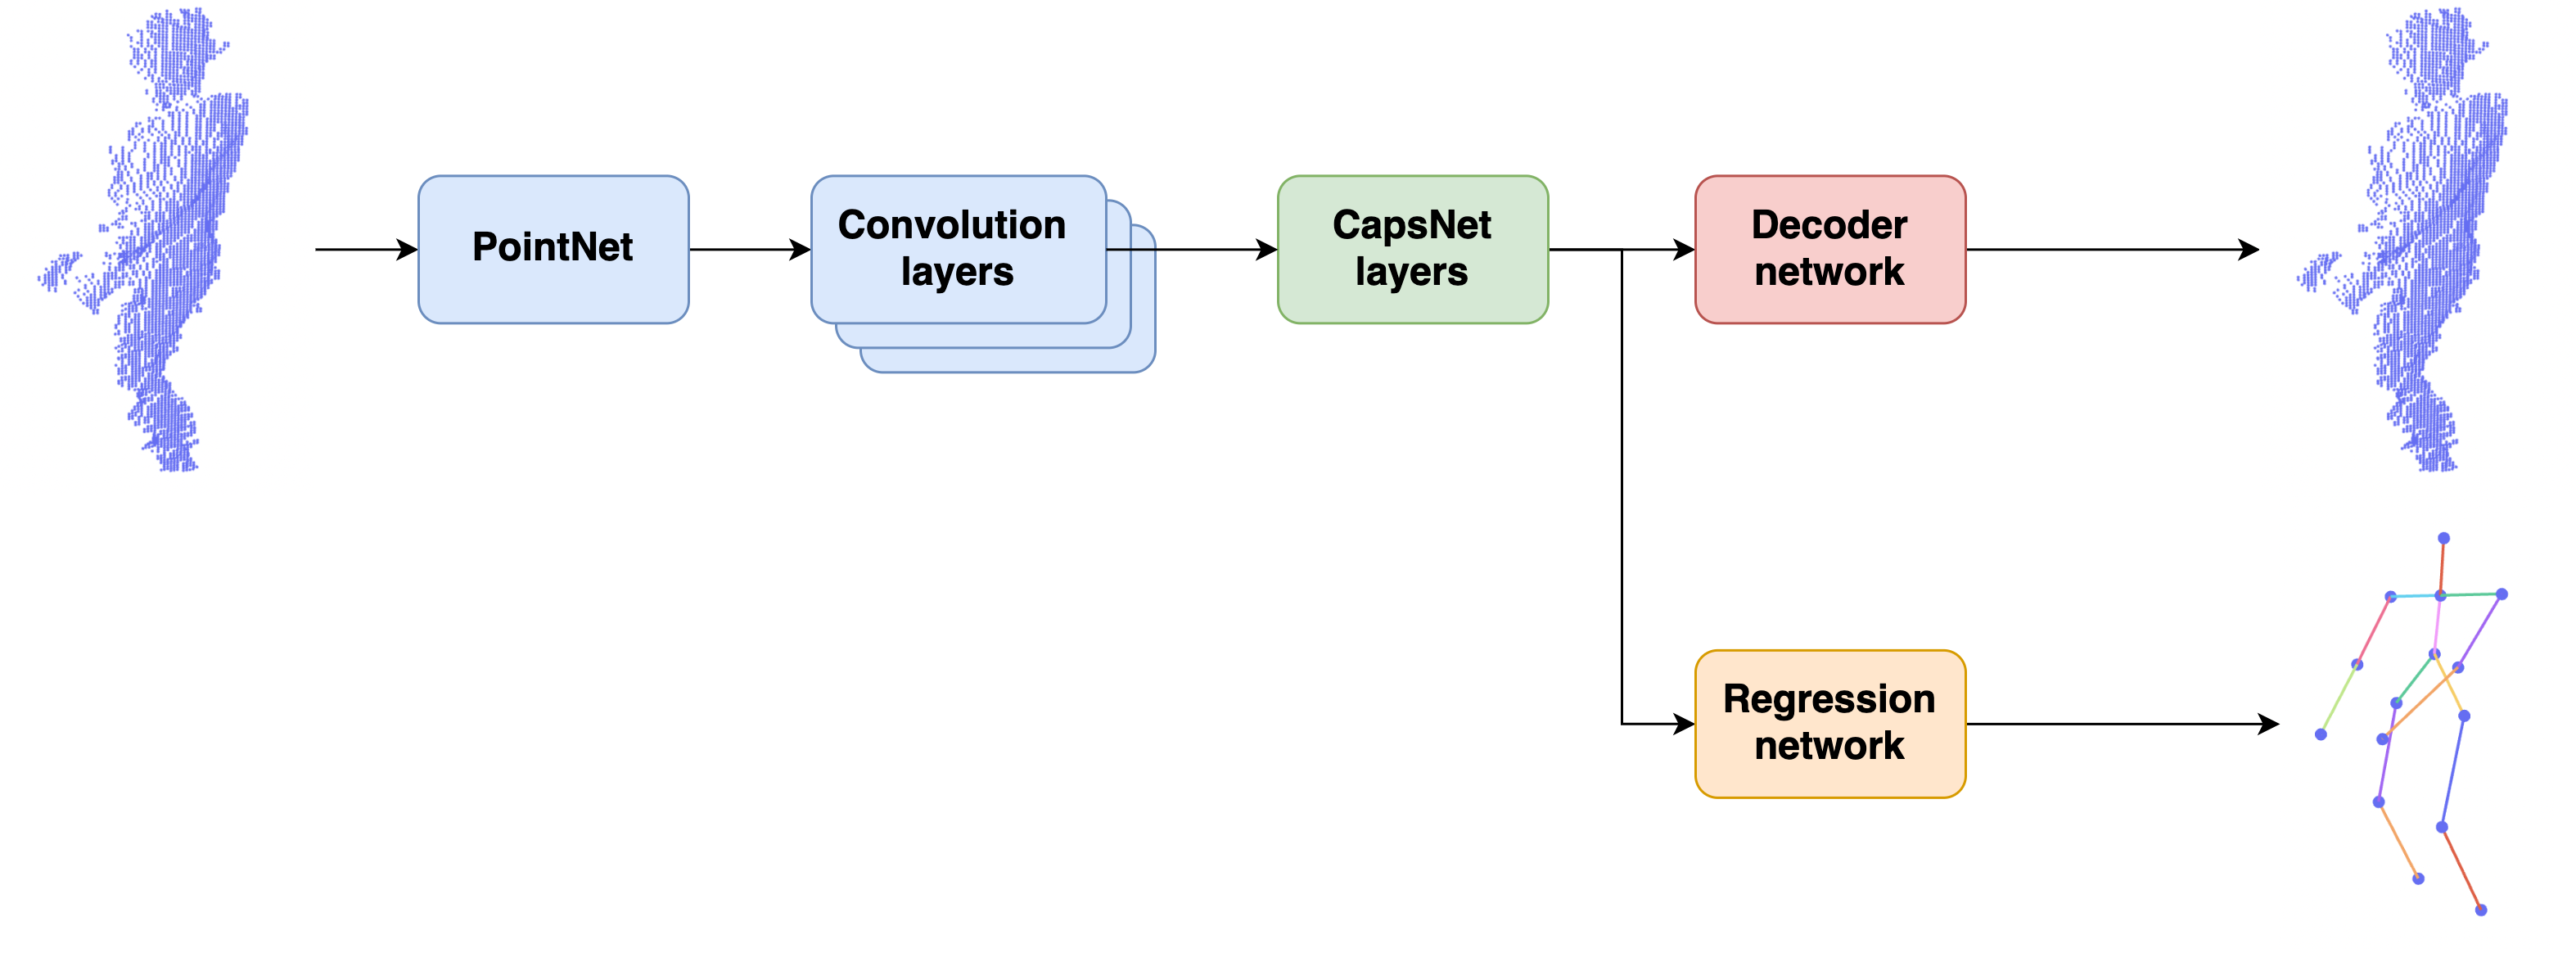
\includegraphics[scale=.125]{Figures/network architecture.png}}
    \caption{Network architecture}
    \label{img:network-architecture}
\end{figure}

% \subsection{Capsule network autoencoder}
% \subsection{Capsule-based regression network}

\subsection{Loss aggregation}
In this work we propose one-stage training based on loss aggregation. 
We will compare results of the training with both two-stage training scheme and simple "loss sum" aggregation strategy.
For the encoder-decoder part of the network the Chamfer distance is used as a loss function. 
The Chamfer distance is defined as:

\begin{equation}
d_{C D}\left(P_{1}, P_{2}\right)=\sum_{x \in P_{1}} \min _{y \in P_{2}}\|x-y\|_{2}^{2}+\sum_{y \in P_{2}} \min _{x \in P_{1}}\|x-y\|_{2}^{2}
\label{eqn:chamfer-distance}
\end{equation}

Where $P_1 \in R^3$ and $P_2 \in R^3$ represent point clouds from the human point cloud and the point cloud recovered from latent capsules.


The regression loss is defined as:

\begin{equation}
    \operatorname{Loss}_{E}(T, J)=\frac{1}{N} \sum_{i=1}^{N}\left(\left\|j_{i}-F\left(t_{i}\right)\right\|^{2}\right)+\lambda\|w\|^{2}
\label{eqn:regression-loss}
\end{equation}
Where $T$ is a feature vector from latent capsules. $J$ is the ground truth human joints. And $F$ is the regression network.

\subsubsection{Baseline: sum of losses}

\subsubsection{TBD loss aggregation}




\section{Network training}
\label{network-training}

 
\chapter{Dataset and evaluation metrics}

\label{Dataset} 
\chapter{Experiments}
\label{Experiments}

In this chapter we describe experiment results based on methodology stated in Chapter~\ref{Methodology}. We use ITOP dataset \parencite{haque_towards_2016} for comparison with different models. To compare our results with existing models we use as a reference such models: RF \parencite{shotton_real-time_2011}, RTW \parencite{ho_yub_jung_random_2015}, IEF \parencite{carreira_human_2016}, VI \parencite{haque_towards_2016}, REN \parencite{chen_pose_2020}, Pose-net \parencite{moon_v2v-posenet_2018}, all of which were overviewed in Chapter~\ref{Related work}.

In Section~\ref{s:one-stage-training} we show our results with one stage straining scheme compared to the two-stage described in Section~\ref{s:one-stage-network-training}.

In Section~\ref{s:results-on-itop} we show the performance of the one-stage training model on the ITOP dataset \parencite{haque_towards_2016}. Also, we compare our results with state-of-the-art models for the same task.

In Section~\ref{s:experiment-noise} we show a comparison of models' performance on a dataset with additional noise described in Section-\ref{s:how-noise-affects-models-performance}. As a reference model we use SOTA model - Pose-net \parencite{moon_v2v-posenet_2018}.

In Section~\ref{s:experiment-lack-of-data} we compare our proposed model with the SOTA Pose-net model with truncated dataset size to assess models' convergence.

% -------------------------- Experiment setup -------------------------
\section{Experiment setup}
\label{s:experiment-setup}
In this section, we describe the basic setup for our experiments. Some experiments have additional changes to the training/evaluation pipelines described in dedicated subsections.

All experiments were performed on a server with 8 CPU core, 1 GPU card Nvidia Tesla P100 (16.2 Gb of video memory), and 60 Gb of RAM. As a training framework, Pytorch 1.8.1 was used based on CUDA 10.1 video driver. This setup was powered by the Google Colab backend.

All point clouds from the ITOP dataset were preprocessed according to Section~\ref{Data-preparation}. For threshold filtering and normalization we use NumPy Python library, and for point cloud clusterization and human extraction we use C++ PCL \parencite{noauthor_strawlabpython-pcl_2021} library with Python bindings. After preprocessing we reduce the number of points in the human cloud to 2,000 to speed up the model's training time. The Adam optimizer \parencite{kingma_adam_2017} was used for all experiments. The initial learning rate is $lr = 10^{-4}$ with learning rate decay of $10^{-1}$ each $30$ epochs. The average number of epoch to a fully trained model is $~80$, after this time of epoch our model starts to oscillate on the plateau. The average training time in such a setup is 16 machine hours. The batch size of $12$ was used. After each epoch of the training dataset, we run evaluation pipelines to measure the model's performance, on each evaluation run we save such metrics: reconstruction loss (Formula~\ref{eqn:chamfer-distance}), regression loss (Formula~\ref{eqn:regression-loss}), total loss (Formula~\ref{eqn:aggregated-loss}), mAP for $10\  cm$ distance (Formula~\ref{eqn:dataset-metric-map}). For visualization purposes, we also save input and reconstructed point clouds ($P$ and $\hat{P}$ accordingly).


% -------------------------- ONE STAGE TRAIN -------------------------
\section{Effectiveness of one stage training}
\label{s:one-stage-training}
In this section, we compare our proposed approach of a one-stage training scheme with the original two-stage one \parencite{wu_3d_2020}.

The main objective of one-stage training is to reduce the number of hyperparameters and speed up training via aggregation strategy of reconstruction and regression losses in the network. There are two experiments conducted on the original architecture described by \cite{wu_3d_2020} and our proposed method described in Section~\ref{s:one-stage-network-training}.

At first, we train capsule networks with a two-stage setup. For the first stage, we use the setup described in Section~\ref{s:experiment-setup} and freeze the regression part of the network, thus we train only the reconstruction part. In this setup, we run 70 epochs and save the model. The second stage uses weights of the model from the first step, but now freeze feature extractor and reconstruction parts of the network and train only regression. In this setup, only 20 epochs are needed to fully converge.

The second experiment adopts our proposed solution with loss aggregation. In this experiment, we train all the networks at once, without freezing any layers. This experiment is done according to Section~\ref{s:experiment-setup}.

The comparison of the two experiments is shown in Table~\ref{tab:two-stage-vs-one-stage}. 

\begin{table}[H]
    \caption{The comparison of one stage and two stage training pipeline (based on Formula~\ref{eqn:dataset-metric-map} metric)}
    \label{tab:two-stage-vs-one-stage}
    \centering
    \begin{tabular}{l l l l}
    \toprule
    \tabhead{Dataset} & \tabhead{Two stage training} & \tabhead{One state training (our method)} & \tabhead{Difference} \\
    \midrule
    ITOP front view & 79.6\%  & 83.1\%  & 3.5\% \\
    ITOP side view & 70.8\% & 74.2\%  & 3.4\% \\
    \bottomrule\\
    \end{tabular}
\end{table}


\begin{figure}[!htbp]
    \centerline{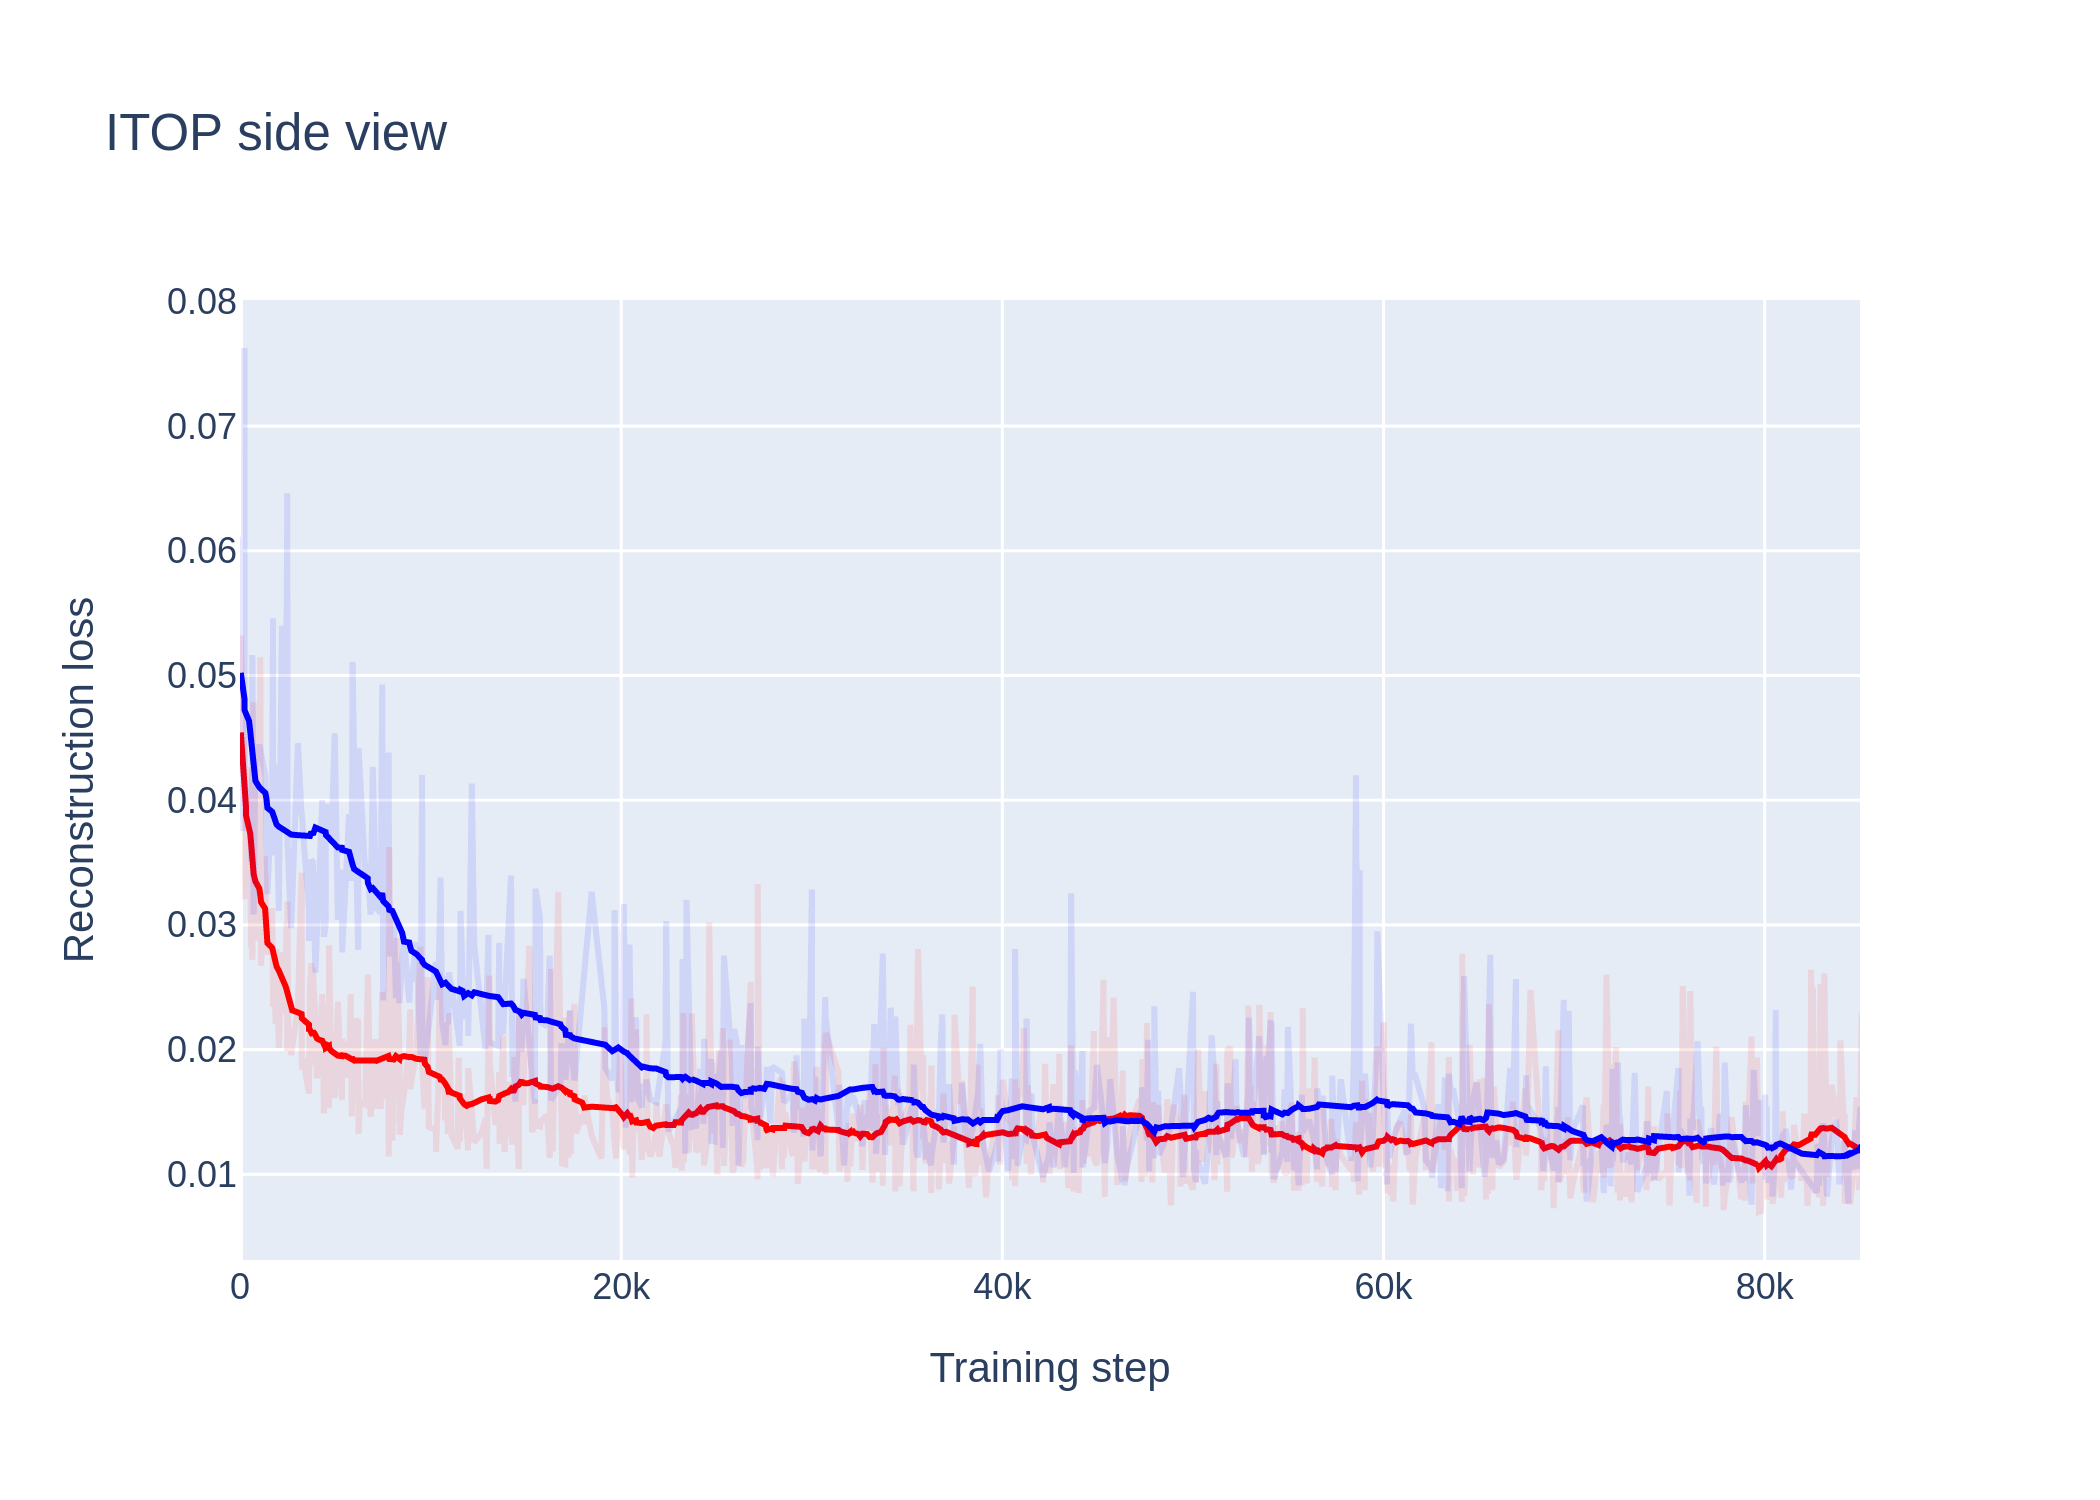
\includegraphics[scale=0.15]{Figures/one-stage-vs-two-stage.png}}
    \caption{Reconstruction loss function for two stage (red) model and one stage model(blue)}
    \label{img:one-stage-vs-two-stage-reconstruction}
\end{figure}

\begin{figure}[htbp]
    \centerline{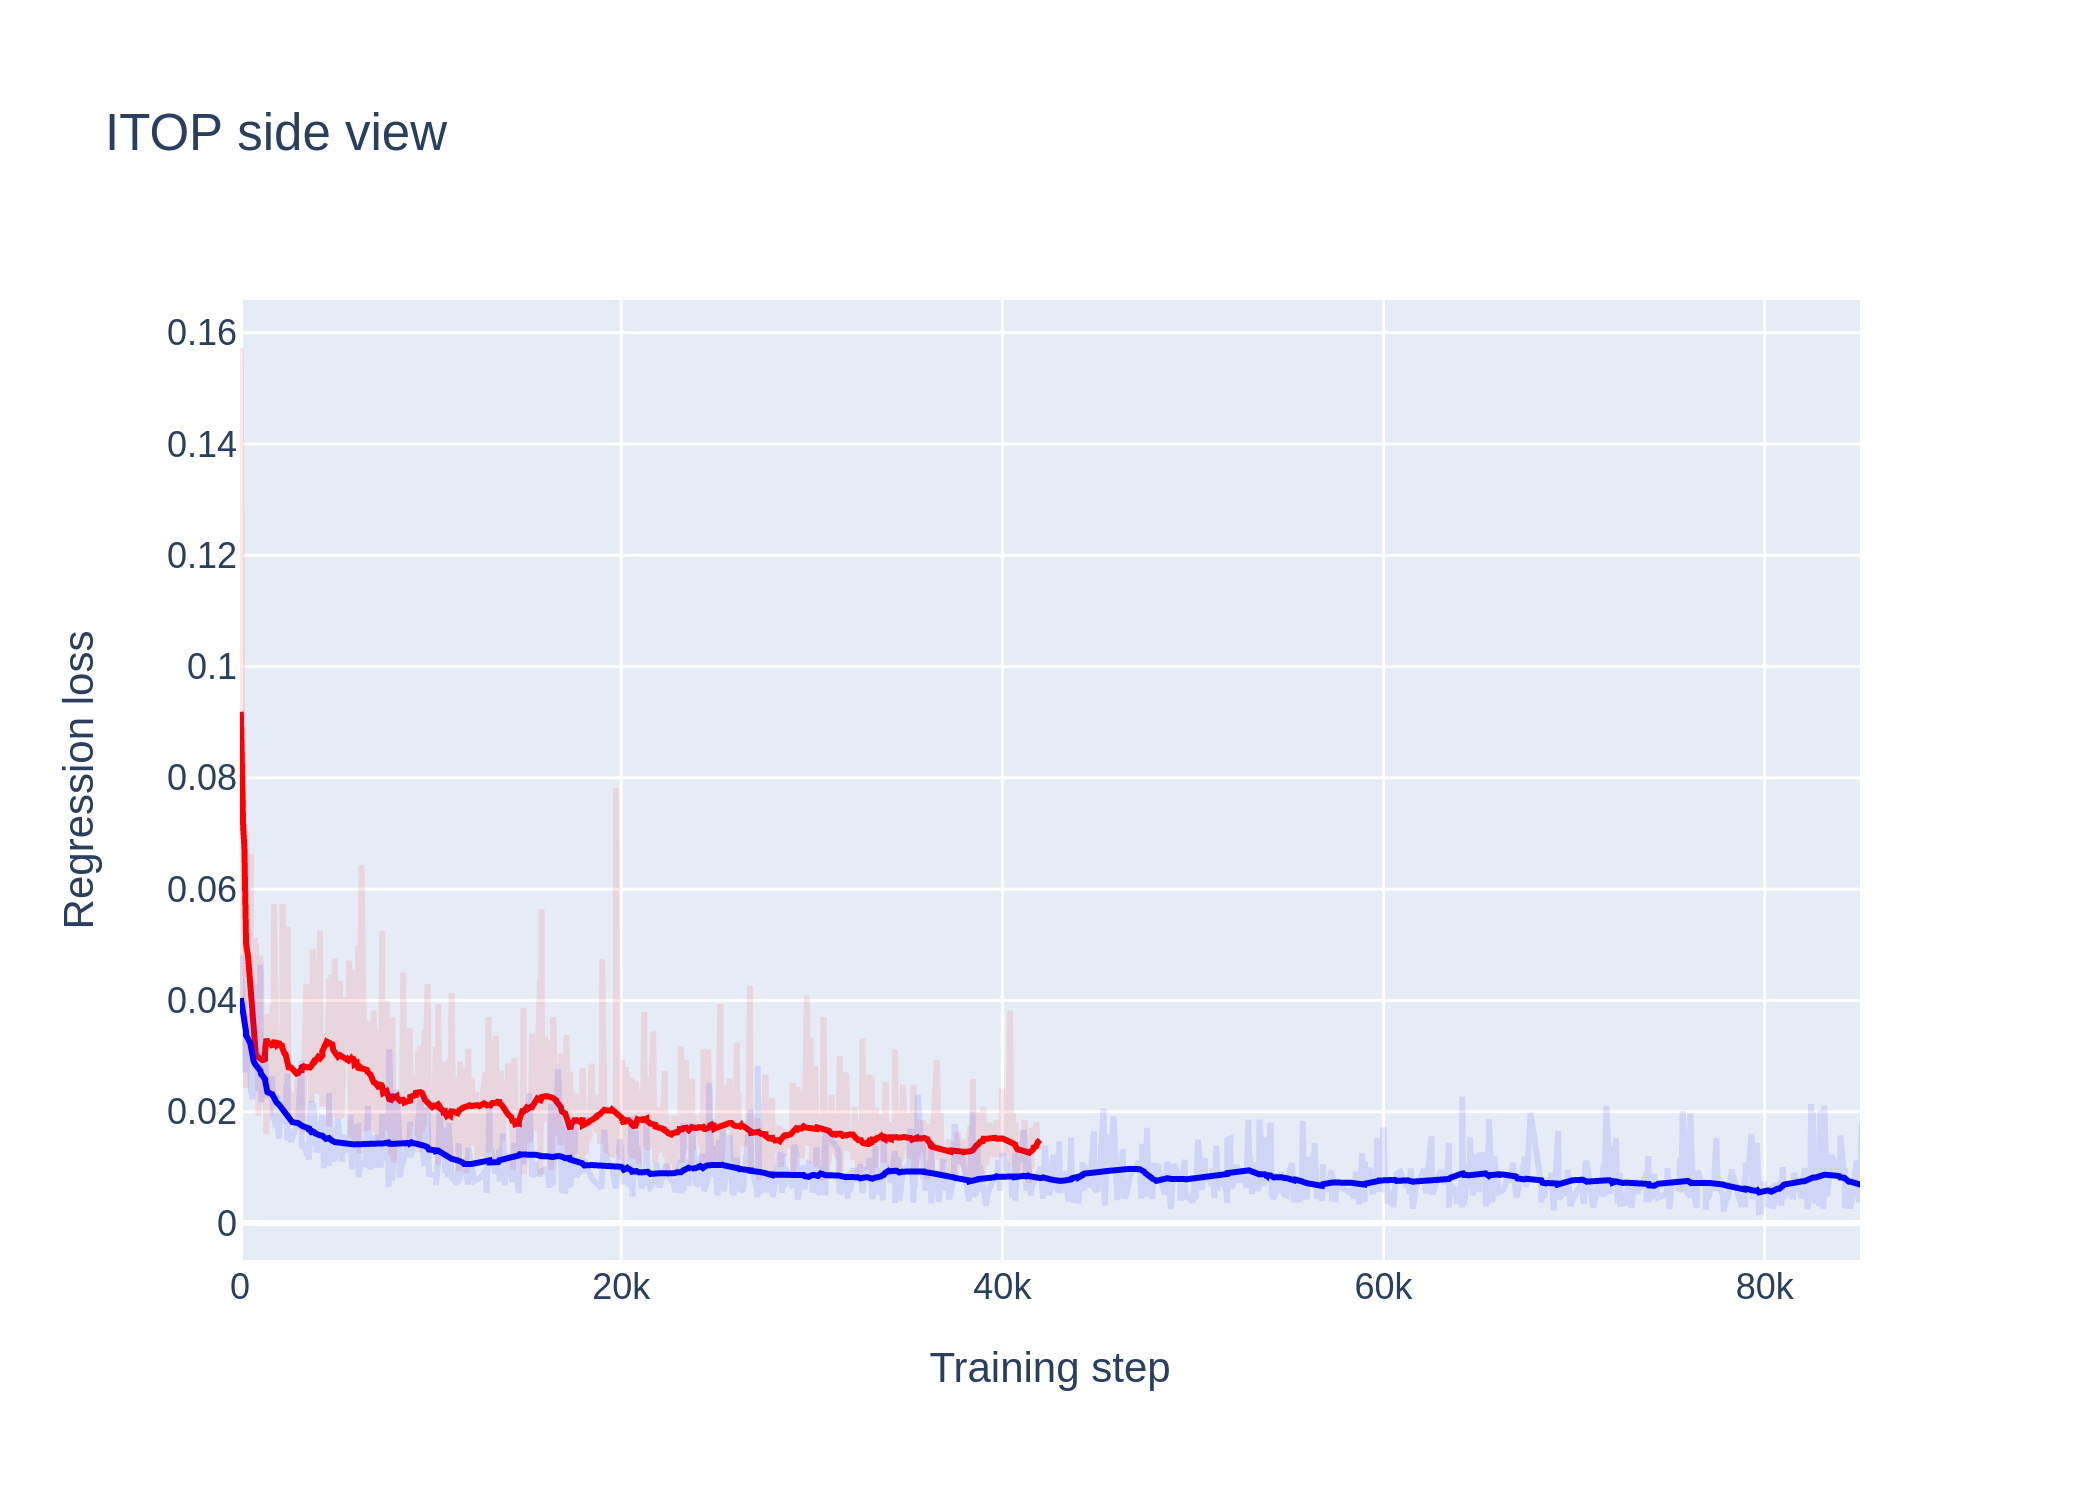
\includegraphics[scale=0.15]{Figures/one-stage-vs-two-stage-regression.png}}
    \caption{Regression loss function for two stage (red) model and one stage model(blue)}
    \label{img:one-stage-vs-two-stage-regression}
\end{figure}

\begin{figure}[htbp]
    \centerline{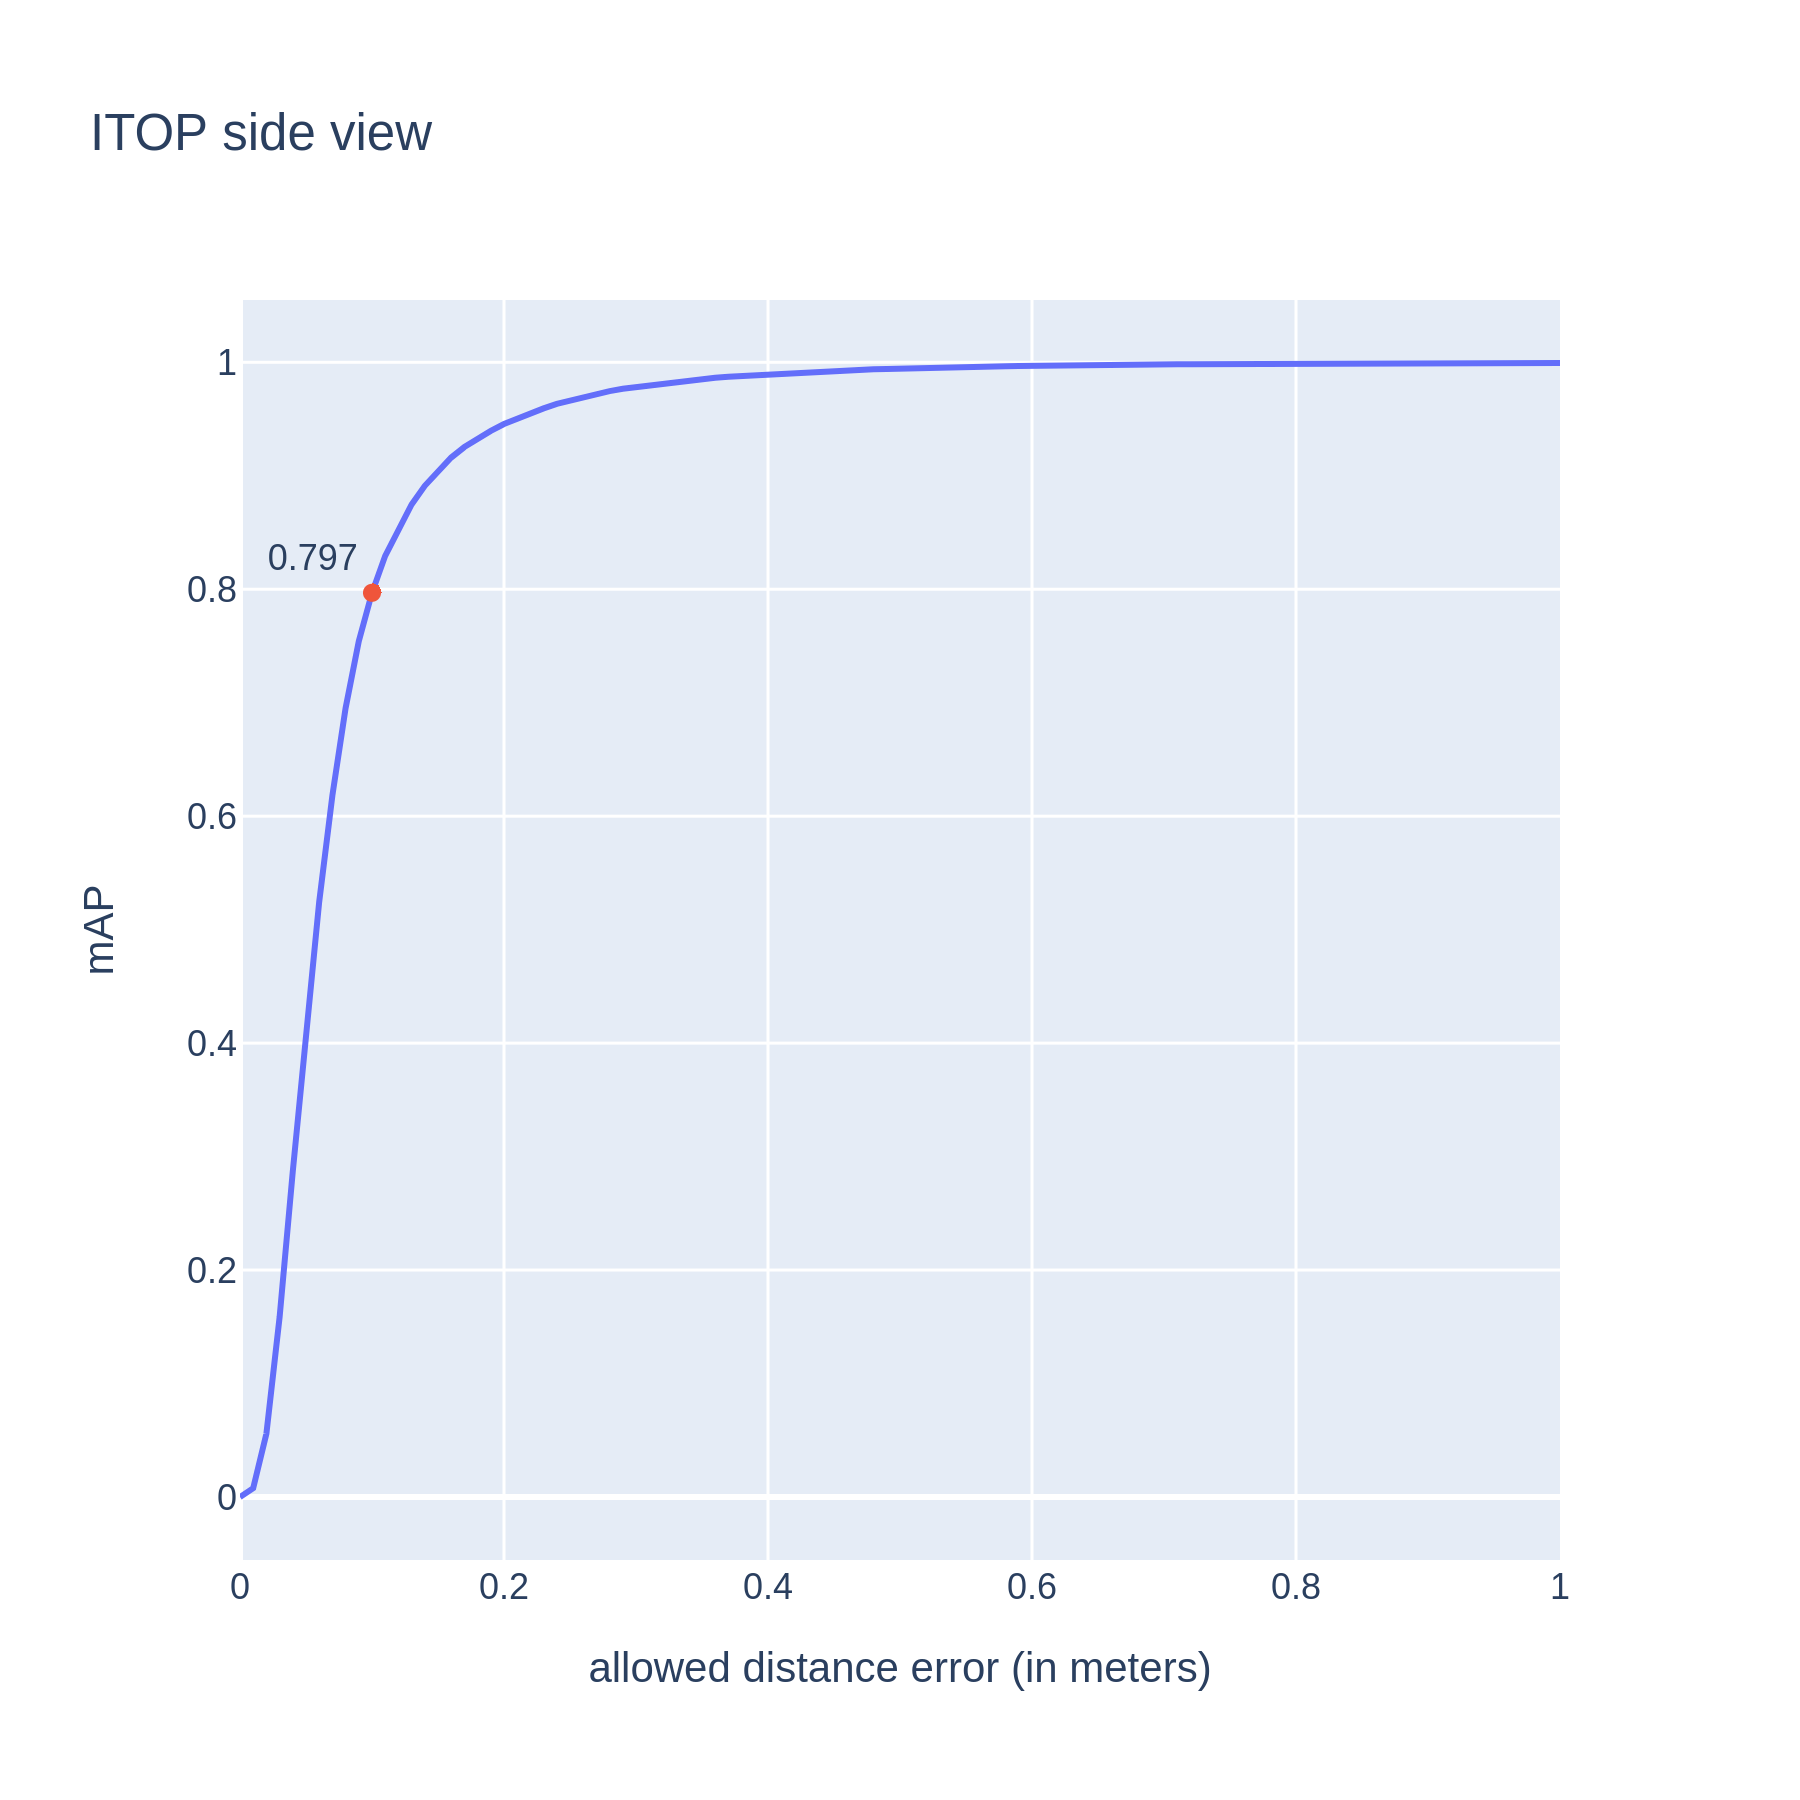
\includegraphics[trim=50 100 50 100,clip,scale=0.15]{Figures/two-stage-map.png}}
    \caption{Two stage model for side view. mAP for different distance errors for two stage model. 10 cm distance mAP is highlighted}
    \label{img:two-stage-map}
\end{figure}

\begin{figure}[htbp]
    \centerline{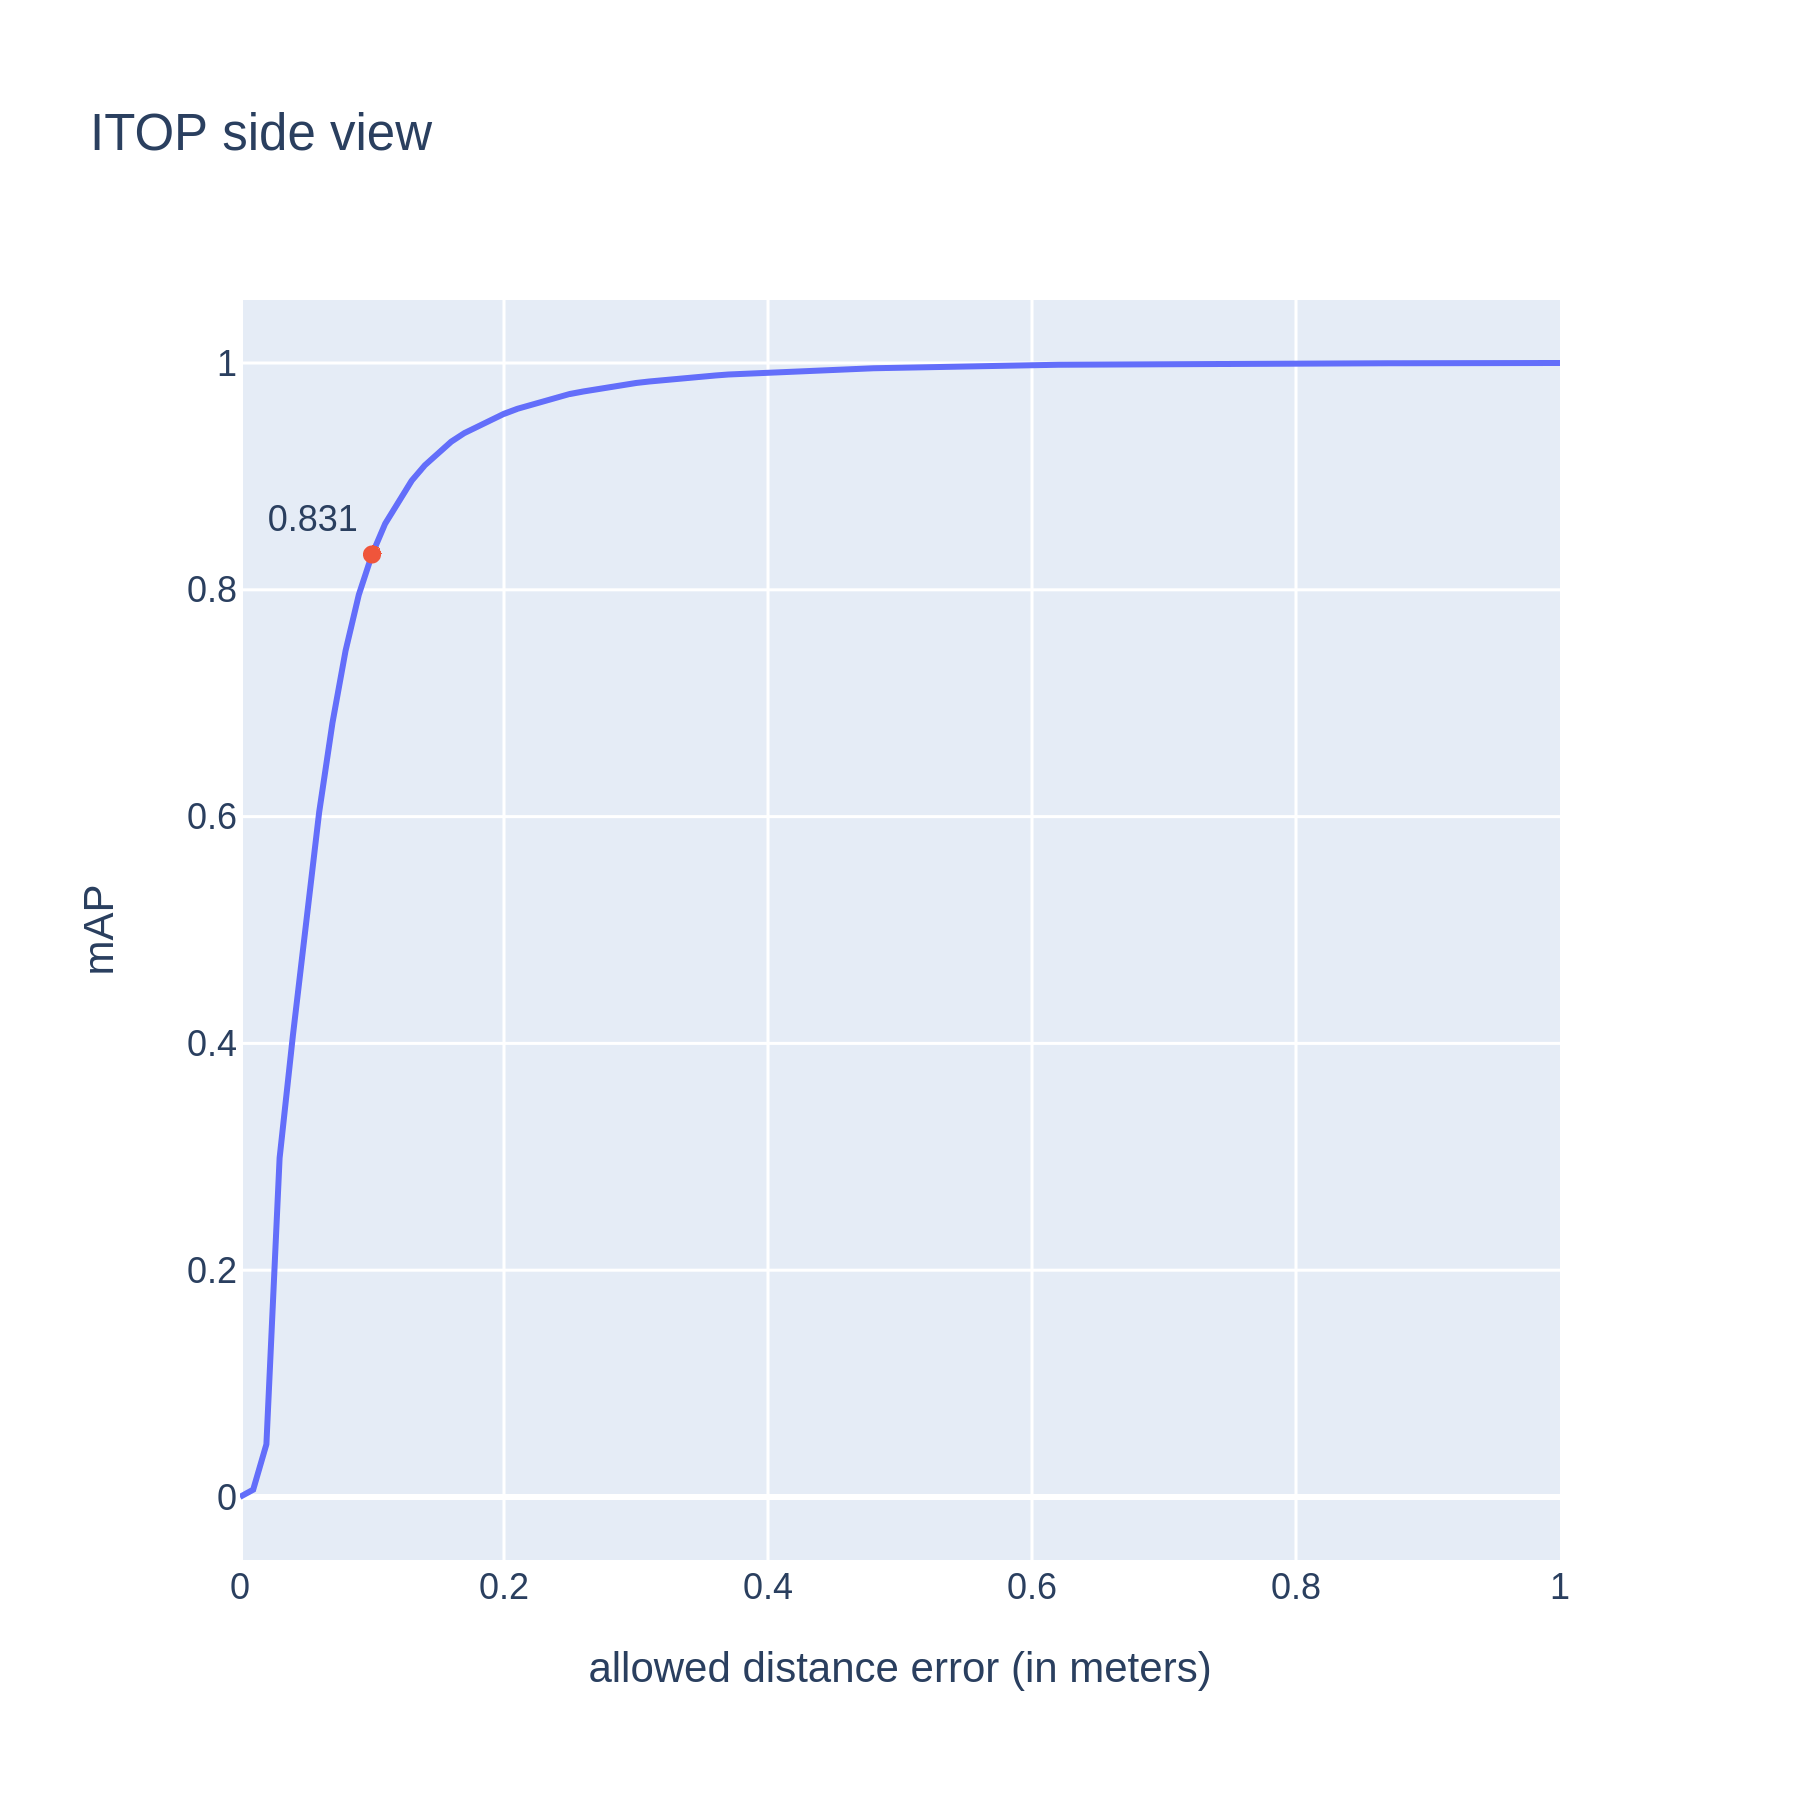
\includegraphics[trim=50 100 50 100,clip,scale=0.15]{Figures/one-stage-map.png}}
    \caption{One stage model for side view. mAP for different distance errors for two stage model. 10 cm distance mAP is highlighted}
    \label{img:one-stage-map}
\end{figure}


\begin{figure}[htbp]
    \centerline{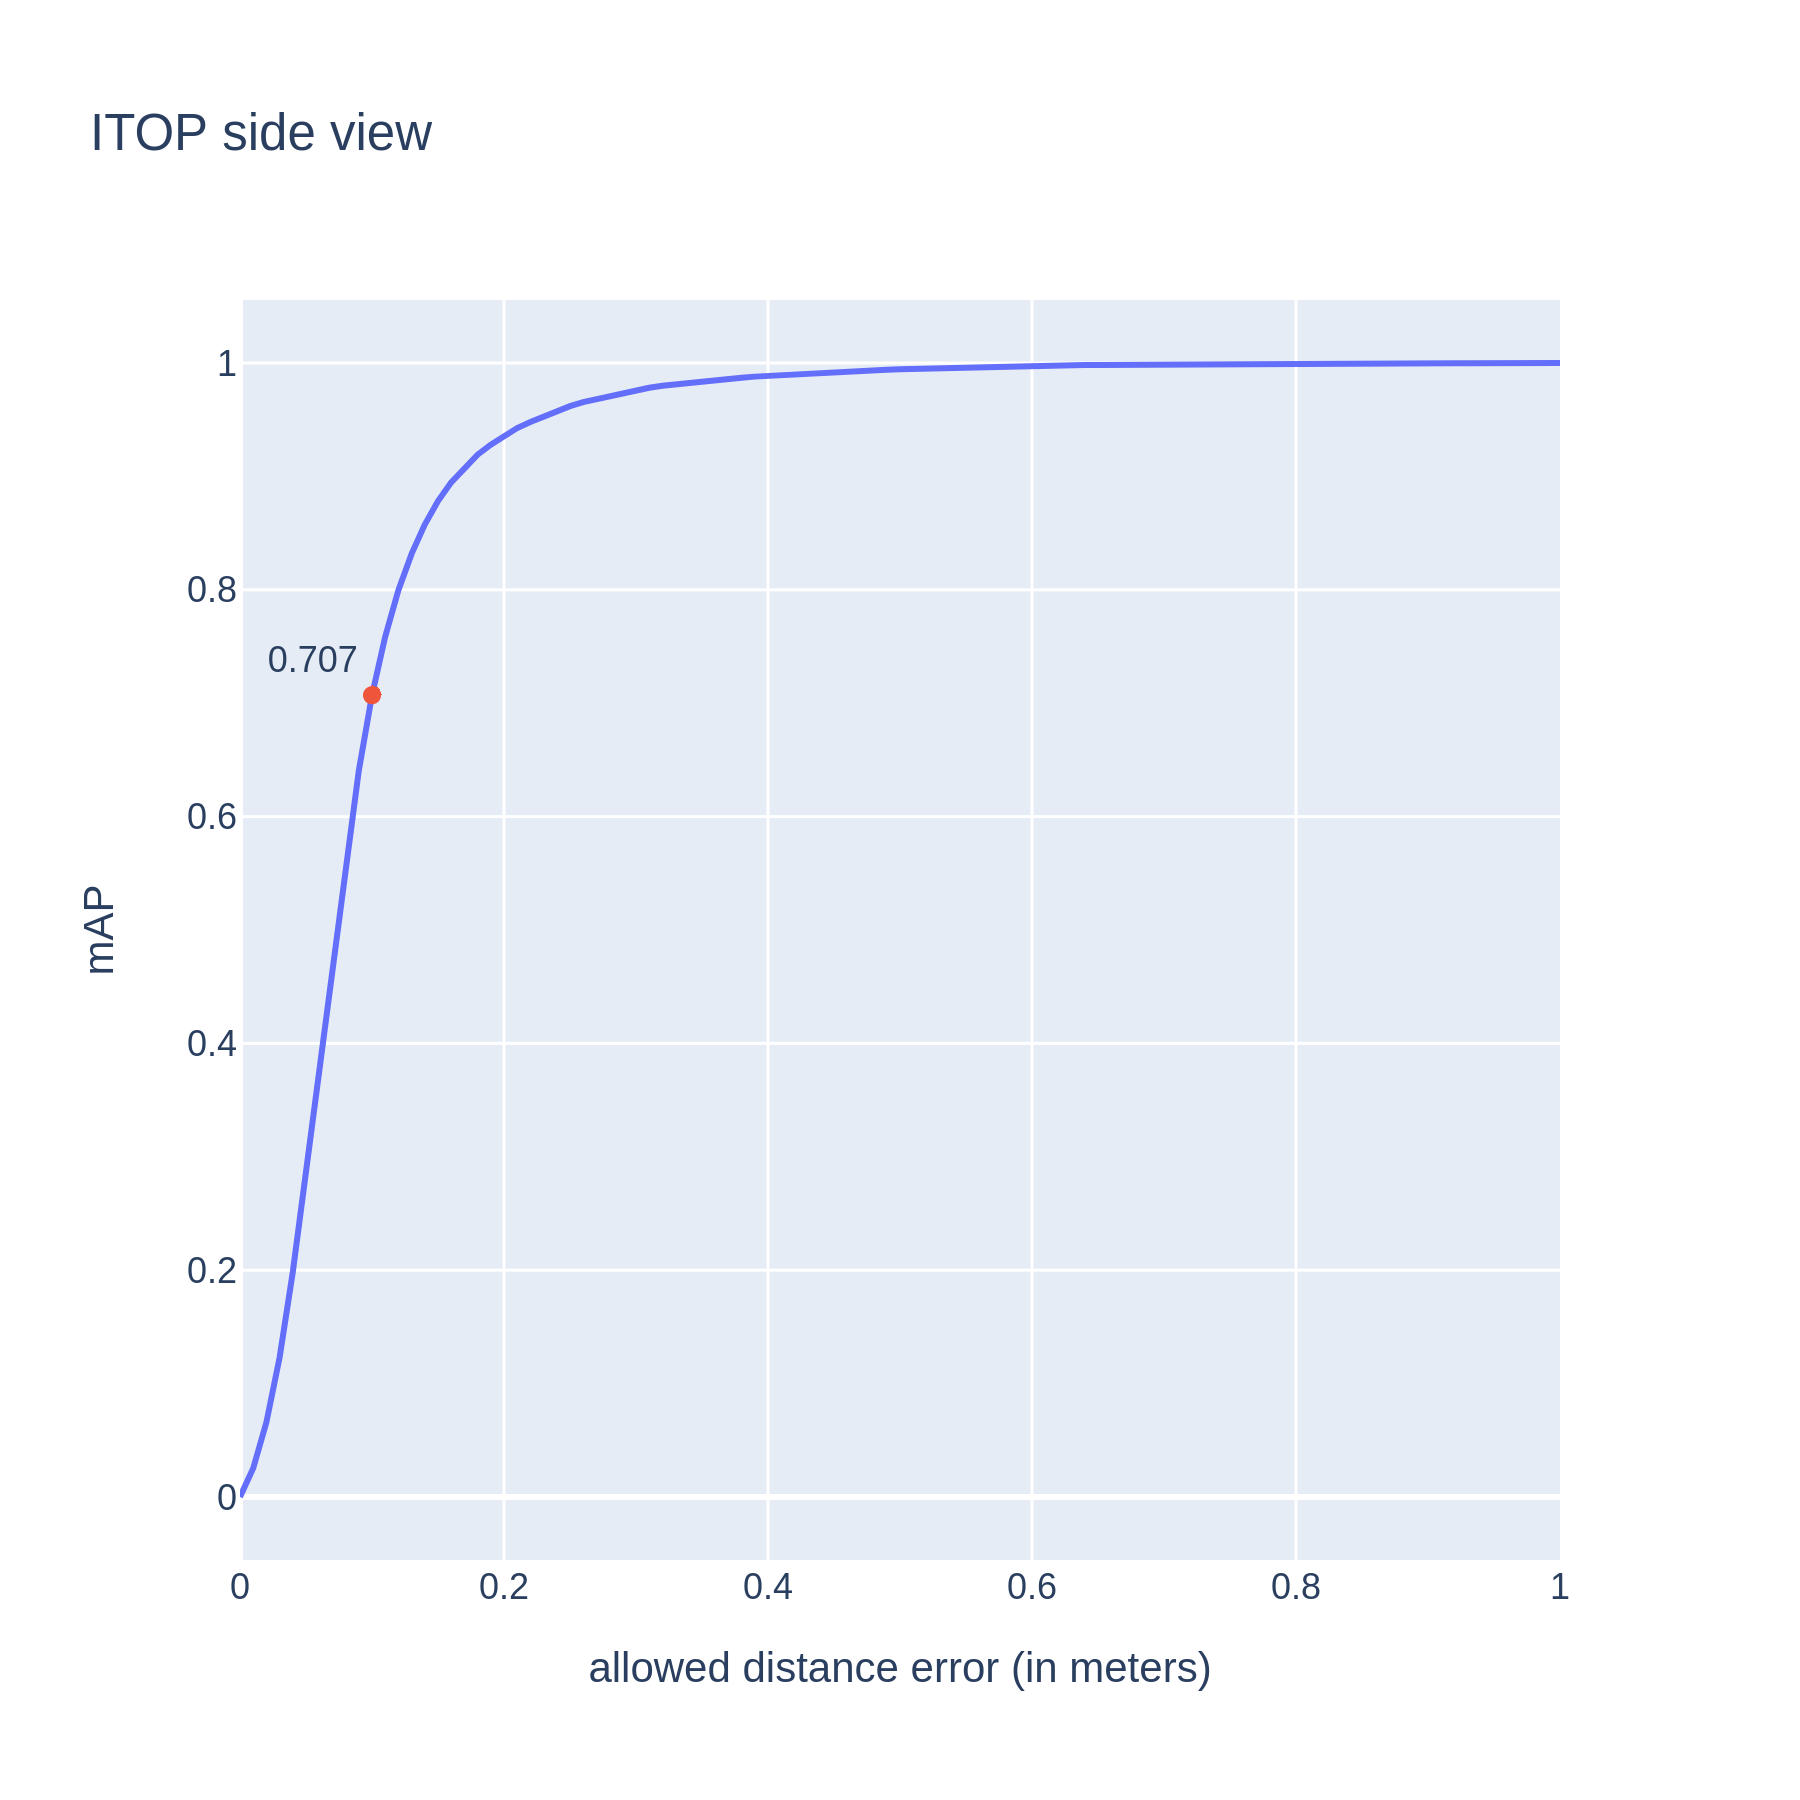
\includegraphics[trim=50 100 50 100,clip,scale=0.15]{Figures/two-stage-map-top-view.png}}
    \caption{Two stage model for top view. mAP for different distance errors for two stage model. 10 cm distance mAP is highlighted}
    \label{img:two-stage-map-side-view}
\end{figure}

\begin{figure}[htbp]
    \centerline{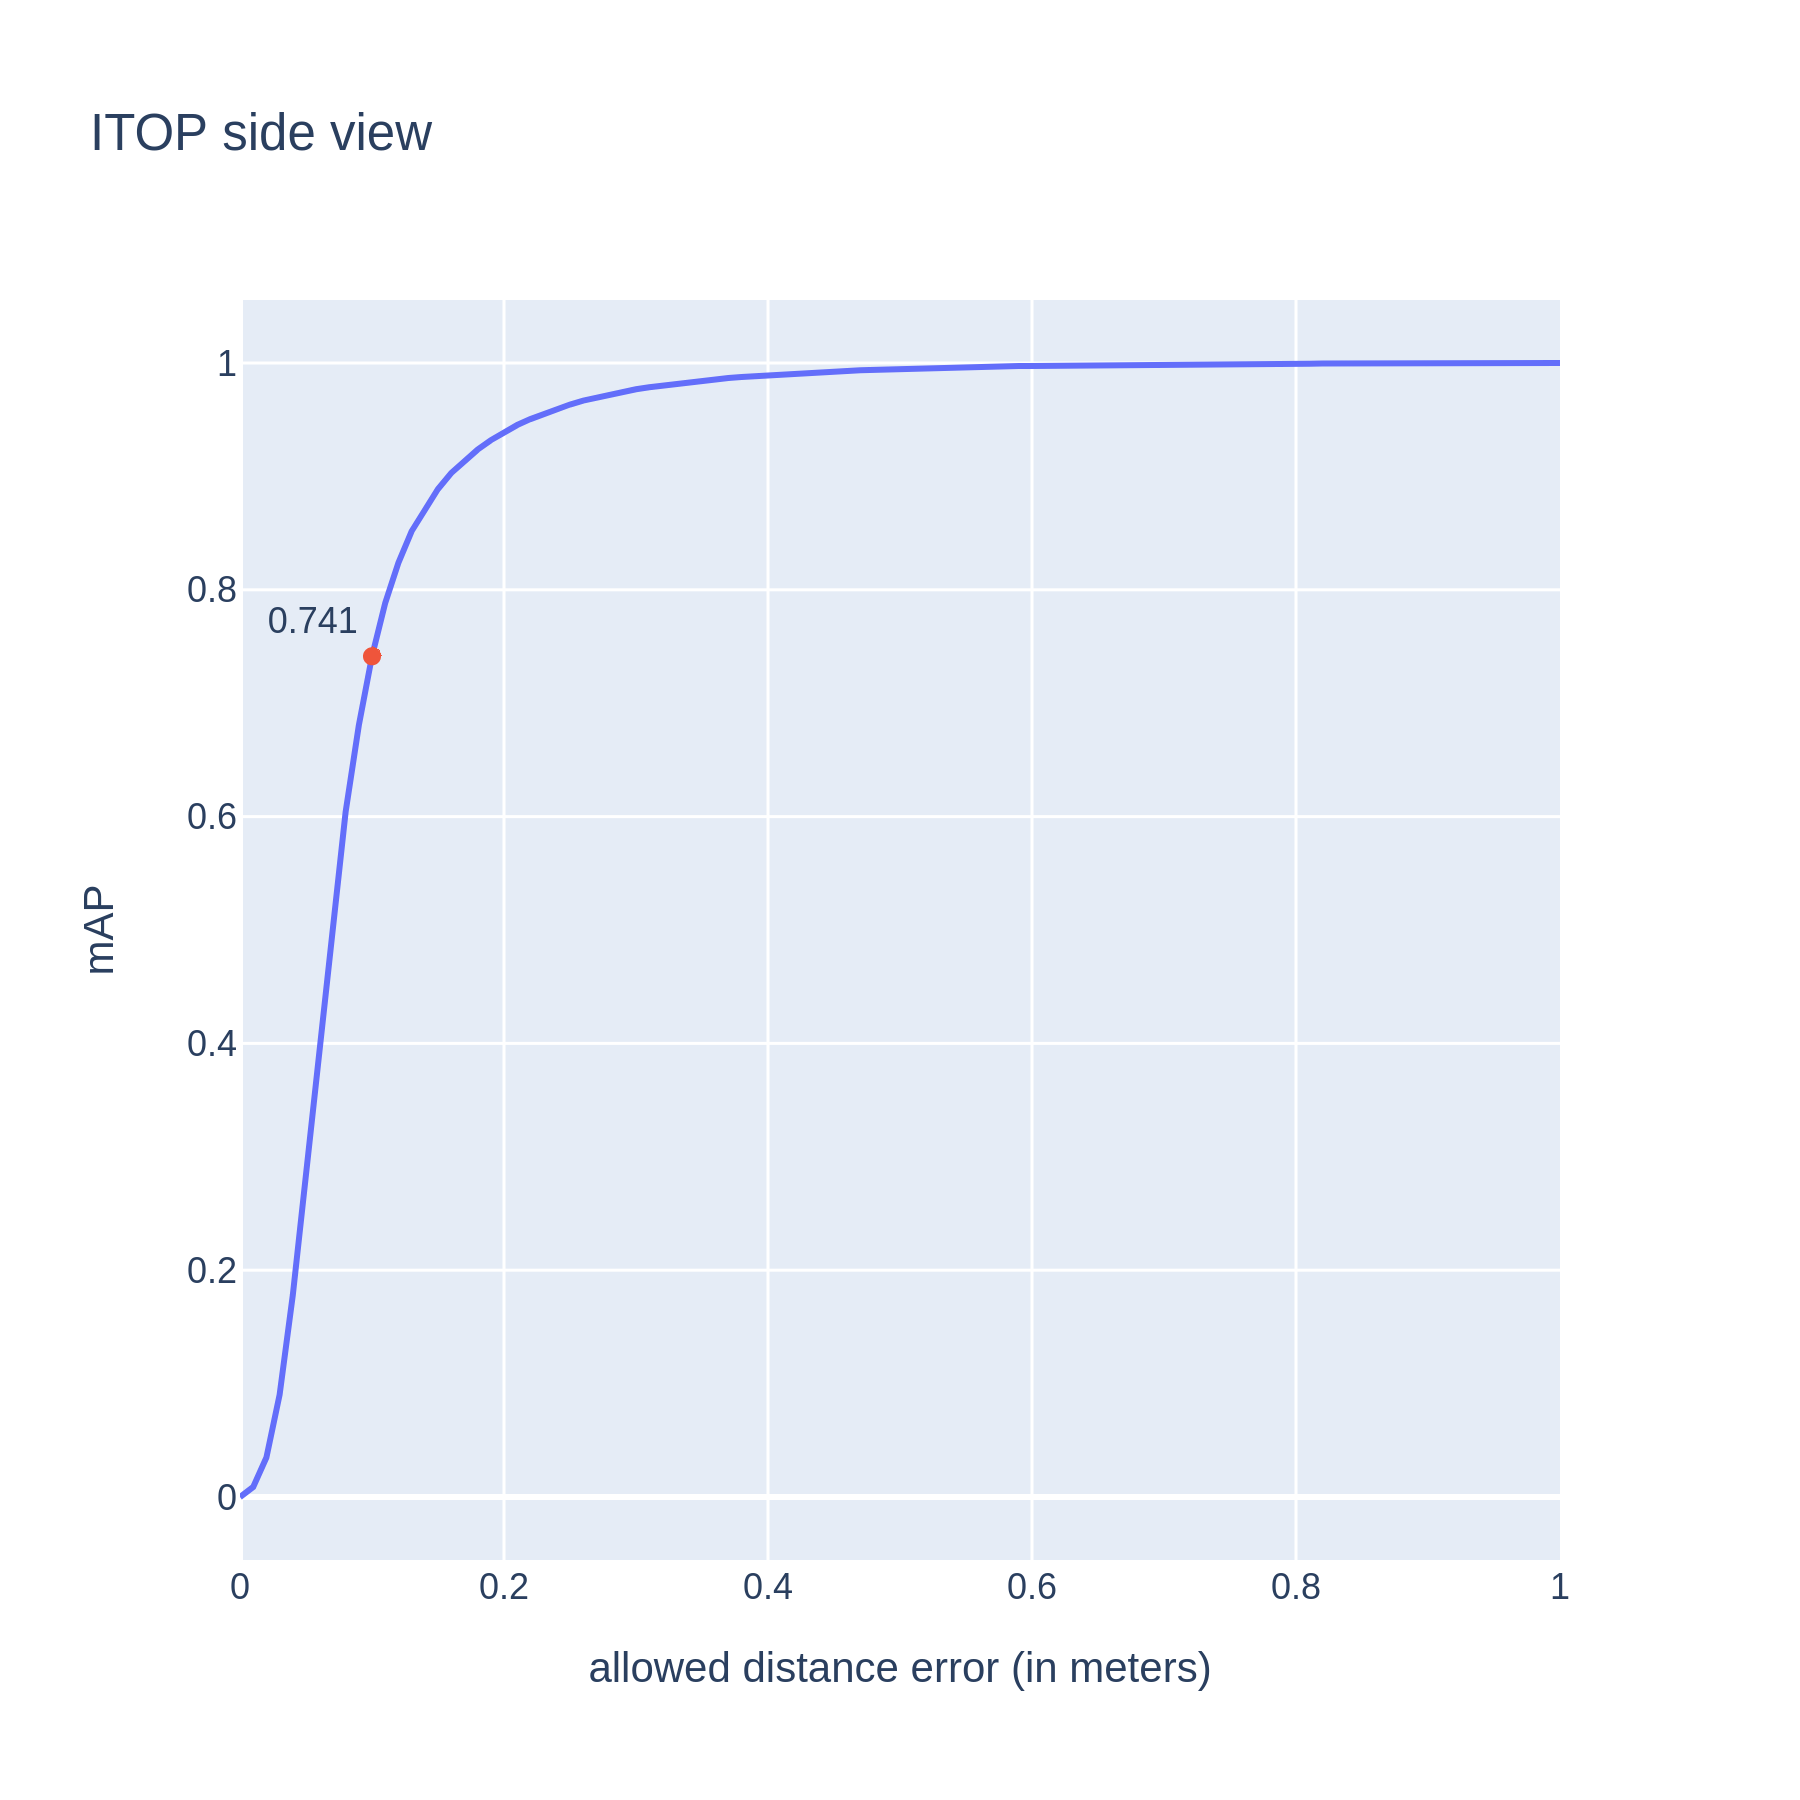
\includegraphics[trim=50 100 50 100,clip,scale=0.15]{Figures/one-stage-map-top-view.png}}
    \caption{One stage model for top view. mAP for different distance errors for two stage model. 10 cm distance mAP is highlighted}
    \label{img:one-stage-map-side-view}
\end{figure}

% -------------------------- ITOP DATASET -------------------------
\section{Results on ITOP dataset}
\label{s:results-on-itop}

We have conducted training and evaluation of our capsule-based model on the ITOP dataset (side and top views). The results of the evaluation, as well as the performance of SOTA models, are shown in Table~\ref{tab:itop-side-view} for side view, and in Table~\ref{tab:itop-top-view} for top view.

\begin{table}
    \caption{Comparison of proposed model with SOTA models on ITOP side view dataset}
    \label{tab:itop-side-view}
    \centering
    \begin{tabular}{l|cccccc|c}
    \hline & \multicolumn{6}{|c} { mAP (side-view) } \\
    \hline Body part & RF & RTW & IEF & VI & REN-9x6x6 & PoseNet & Our model \\
    \hline Head & $63.8$ & $97.8$ & $96.2$ & $98.1$ & $98.7$ & $98.29$ & $94.7$\\
    Neck & $86.4$ & $95.8$ & $85.2$ & $97.5$ & $99.4$ & $99.07$ & $96.9$ \\
    Shoulders & $83.3$ & $94.1$ & $77.2$ & $96.5$ & $96.1$ & $97.18$ & $93.7$ \\
    Elbows & $73.2$ & $77.9$ & $45.4$ & $73.3$ & $74.7$ & $80.42$ & $73.9$ \\
    Hands & $51.3$ & $70.5$ & $30.9$ & $68.7$ & $55.2$ & $67.26$ & $58.0$ \\
    Torso & $65.0$ & $93.8$ & $84.7$ & $85.6$ & $98.7$ & $98.73$ & $97.0$ \\
    Hip & $50.8$ & $80.3$ & $83.5$ & $72.0$ & $91.8$ & $93.23$ & $89.5$ \\
    Knees & $65.7$ & $68.8$ & $81.8$ & $69.0$ & $89.0$ & $91.80$ & $88.1$ \\
    Feet & $61.3$ & $68.4$ & $80.9$ & $60.8$ & $81.1$ & $87.6$ & $80.0$ \\
    \hline Mean & $65.8$ & $80.5$ & $71.0$ & $77.4$ & $84.9$ & $88.74$ & $83.1$ \\
    \hline
    \end{tabular}
\end{table}

\begin{table}
    \caption{Comparison of proposed model with SOTA models on ITOP top view dataset}
    \label{tab:itop-top-view}
    \centering
    \begin{tabular}{l|cccccc|c}
    \hline & \multicolumn{6}{|c} { mAP (top-view) } \\
    \hline Body part & RF & RTW & IEF & VI & REN-9x6x6 & PoseNet & Our model \\
    \hline Head & $95.4$ & $98.4$ & $83.8$ & $98.1$ & $98.2$ & $98.4$ & $94.2$ \\
     Neck & $98.5$ & $82.2$ & $50.0$ & $97.6$ & $98.9$ & $98.91$ & $96.0$ \\
     Shoulders & $89.0$ & $91.8$ & $67.3$ & $96.1$ & $96.6$ & $9 6.87$ & $89.2$ \\
     Elbows & $57.4$ & $80.1$ & $40.2$ & $86.2$ & $74.4$ & $79.16$ & $67.6$ \\
     Hands & $49.1$ & $76.9$ & $39.0$ & $85.5$ & $50.7$ & $62.44$ & $48.9$ \\
     Torso & $80.5$ & $68.2$ & $30.5$ & $72.9$ & $98.1$ & $97.78$ & $94.0$ \\
     Hip & $20.0$ & $55.7$ & $38.9$ & $61.2$ & $85.5$ & $86.91$ & $79.3$ \\
     Knees & $2.6$ & $53.9$ & $54.0$ & $51.6$ & $70.0$ & $8 3.28$ & $80.3$ \\
     Feet & $0.0$ & $28.7$ & $62.4$ & $51.5$ & $41.6$ & $69.62$ & $67.4$ \\
    \hline Mean & $47.4$ & $68.2$ & $51.2$ & $75.5$ & $75.5$ & $83.44$ & $74.1$ \\
    \hline
    \end{tabular}
\end{table}

Our proposed model shows competitive results both on ITOP side view and front view. Our model outperforms RF \parencite{shotton_real-time_2011}, RTW \parencite{ho_yub_jung_random_2015}, IEF \parencite{carreira_human_2016} models on both datasets, and aslo VI \parencite{haque_towards_2016} on side-view only. The model still underperform REN \parencite{chen_pose_2020}, Pose-net \parencite{moon_v2v-posenet_2018} models.

Our model gives good results on head, neck, shoulders, torso body parts, and struggle to estimate hands and feet. It's difficult for a model to predict a key joint that is located in a relatively small point cloud (compared to whole-body).


In the Figure~\ref{img:reconstruction-example} we could see how the model reconstructs the human body with each epoch. On first epochs, the model outputs just a random point cloud, and with each new epoch, it trains to reproduce the input point cloud. As we can see from $d)$ in Figure~\ref{img:reconstruction-example} on epoch 60 the model's approximation is pretty solid.

\begin{figure}[htbp]
    \centerline{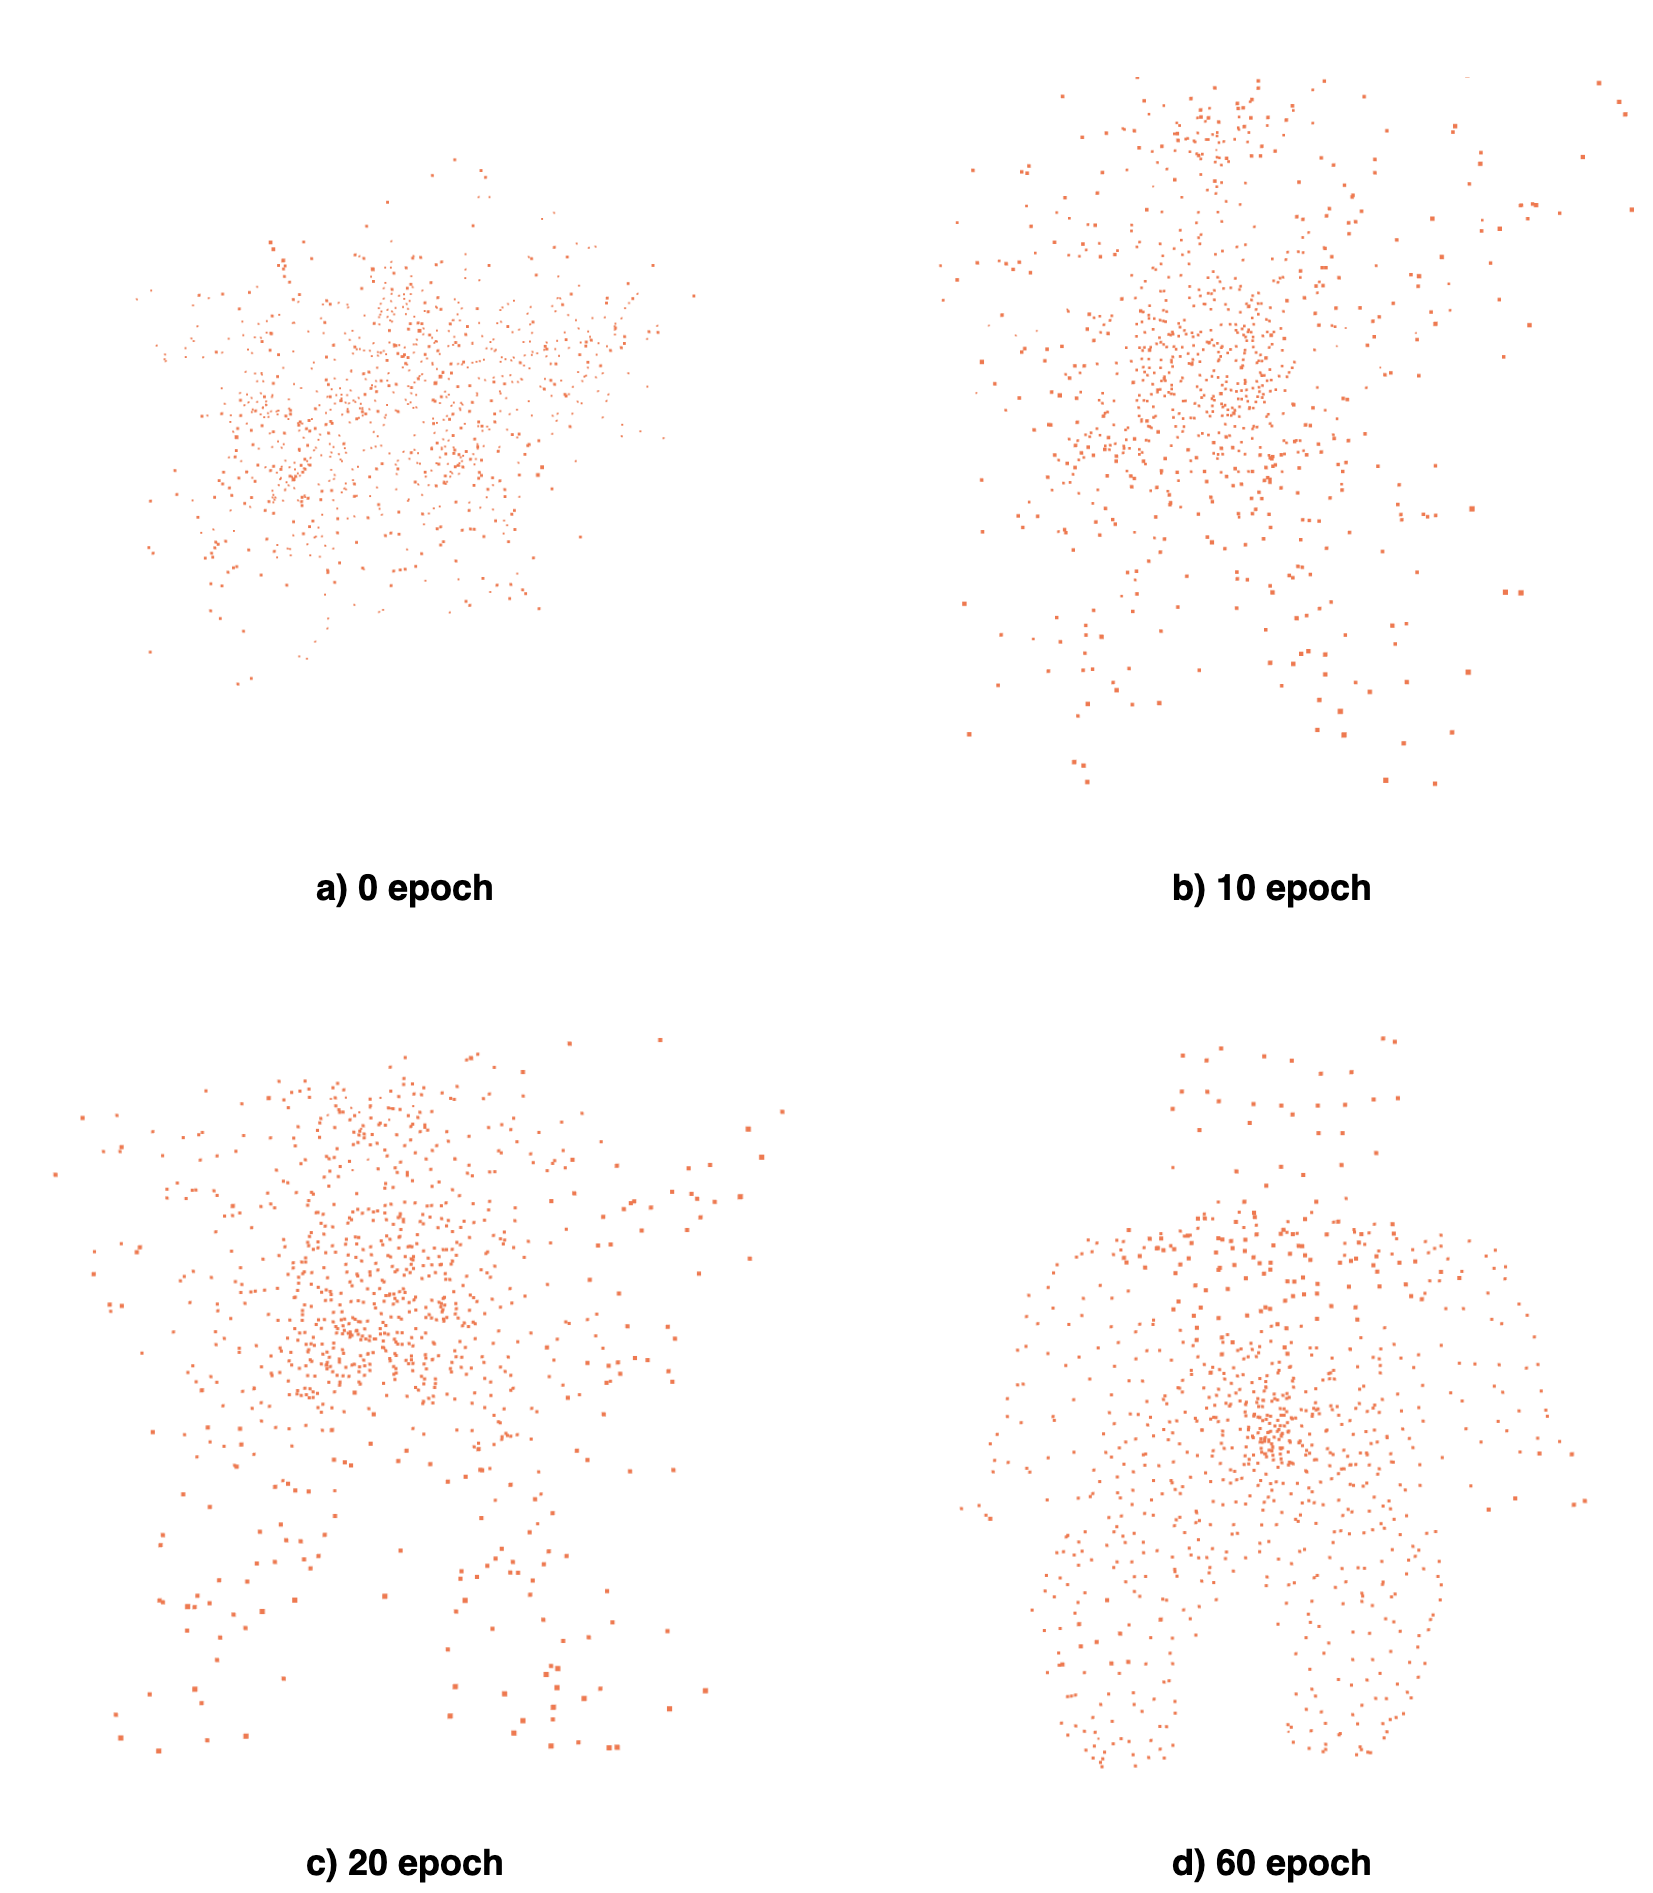
\includegraphics[scale=0.25]{Figures/reconstruction-example.png}}
    \caption{One stage model for top view. mAP for different distance errors for two stage model. 10 cm distance mAP is highlighted}
    \label{img:reconstruction-example}
\end{figure}

% -------------------------- NOISE IN DATA -------------------------

\section{How noise affects models' performance}
\label{s:experiment-noise}

In this section, we evaluate a capsule-based model (proposed solution) and a reference model (PoseNet) on a dataset with a different amount of noise. The experiment's description is covered in Section~\ref{s:how-noise-affects-models-performance}.

We use Gaussian noise and uniform noise as a mixin to the initial data. For the Gaussian noise, we add noise with a probability of $\frac{1}{3}$ (to roughly 30\% of points). We use two types of values for $\sigma$ - $0.1$ for mild noise and $0.2$ for more aggressive.

For uniform distribution we use constant number of additional points $N_P = 300$. That is roughly $15\%$ of additional points out of mean human point cloud size.
In Figure~\ref{img:human-with-noisy-data} is shown an example of human point clouds with additional noise. We don't add noise to ground truths key joints.

\begin{figure}[htbp]
    \centerline{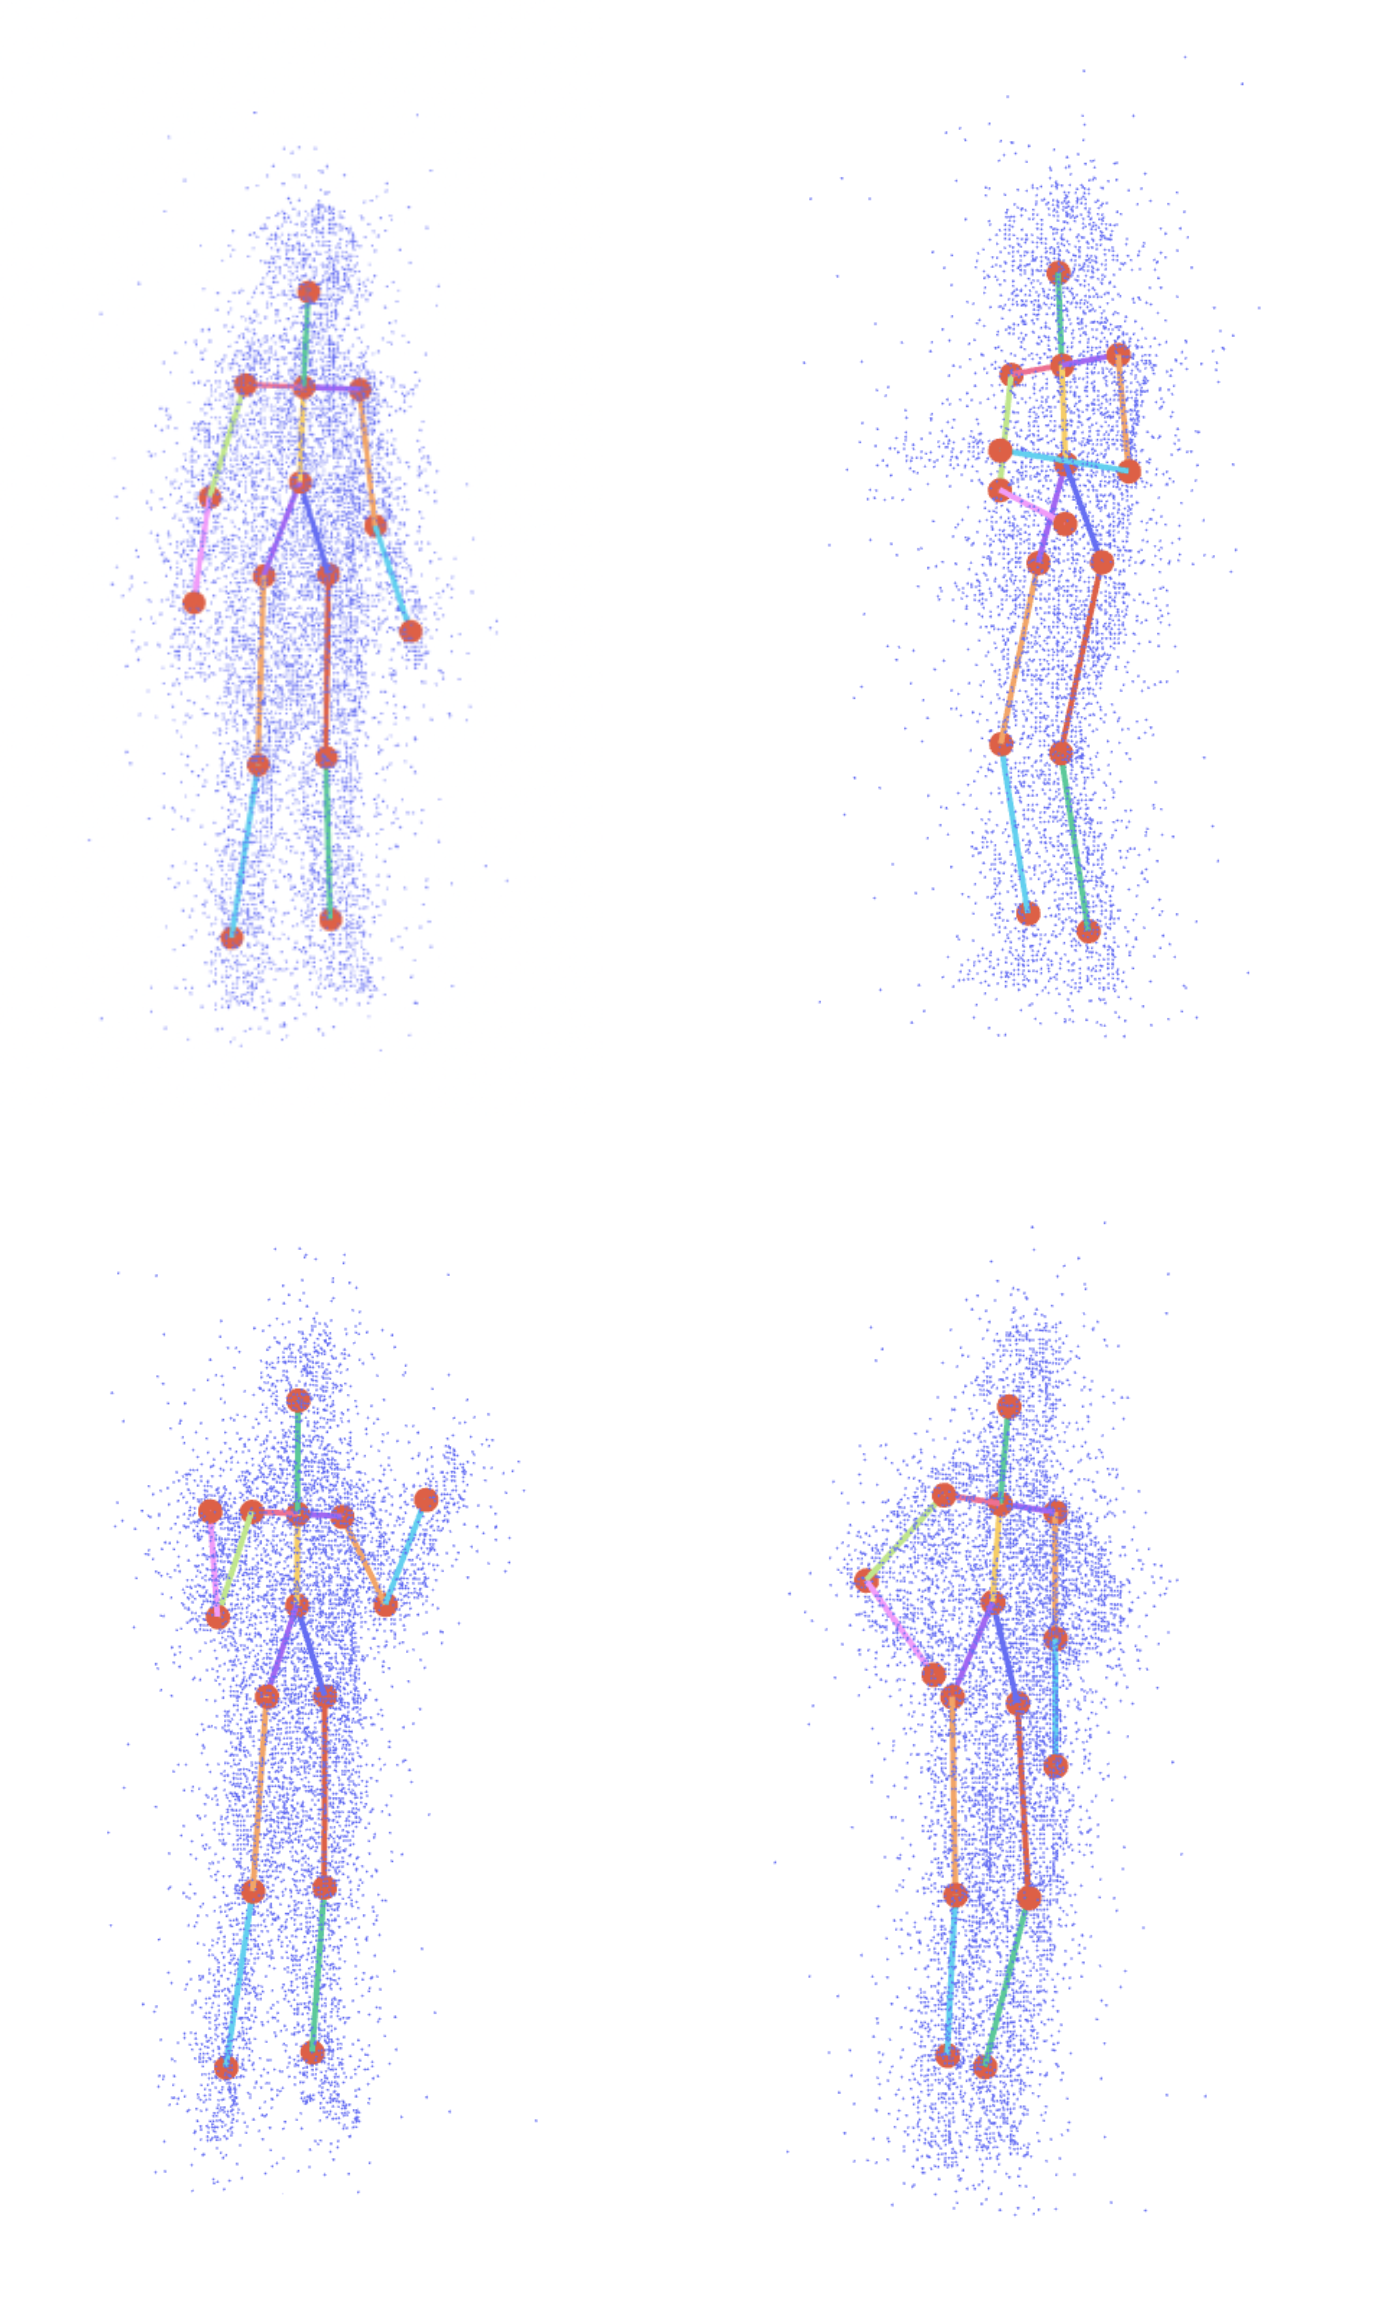
\includegraphics[scale=0.18]{Figures/human-with-noise.png}}
    \caption{Example of human points clouds with added noise. $\sigma - 0.1$, $N_P = 300$}
    \label{img:human-with-noisy-data}
\end{figure}

As for the capsule-based model we use the model trained on the ITOP side view dataset from the Experiment~\ref{s:results-on-itop}. We will use the ITOP side view dataset as a benchmark for this experiment.

As for reference model we use pretrained\footnote{\url{https://github.com/mks0601/V2V-PoseNet_RELEASE}} PoseNet.

We inference the ITOP side view dataset with different noise parameters for both models and measure mAP for each experiment. All experiments are collected in Table~\ref{tab:noise-table-comparison}.

\begin{table}[H]
    \caption{The comparison of capsnet model and PoseNet on dataset with different amount of noise on ITOP side view dataset}
    \label{tab:noise-table-comparison}
    \centering
    \begin{tabular}{l l l l l}
    \toprule
    \tabhead{Noise setup} & \tabhead{PoseNet} & \tabhead{CapsNet} & \tabhead{PoseNet difference} & \tabhead{CapsNet difference}  \\
    \midrule
    No noise (reference) & 86.2\%  & 83.1\%  & 0\% & 0\% \\
    $\sigma=0.1, N_P = 0$ & 82.1\%  & 81.6\%  & 4.1\% & 1,5\% \\
    $\sigma=0, N_P = 300$ & 84.9\%  & 81.9\%  & 1,3\% & 1,2\% \\
    $\sigma=0.1, N_P = 300$ & 80.9\%  & 79.2\%  & 5,3\% & 3,9\% \\
    $\sigma=0.2, N_P = 300$ & 74.5\%  & 70.4\%  & 11,7\% & 12,7\% \\
    \bottomrule\\
    \end{tabular}
\end{table}

The reference value (dataset without noise) for the capsule-based model is $83.1\%$ mAP, and for PoseNet is $86.2\%$ mAP. The PoseNet's results are different compared to Table~\ref{tab:itop-side-view} - $88.74\%$ in table vs $86.2\%$ in our experiment. Such difference could be due to the fact that we don't use an ensemble of PoseNet models for the evaluation. This difference isn't significant for the methodology of our experiment since we use the difference of mAP as a metric.

As we can see capsule-based model performs better on noisy datasets compared to the reference model. For $\sigma = 0.1$ the drop of mAP for capsule network is $1,5\%$ vs $4,1\%$ in PoseNet.

The only experiment where PoseNet outperforms capsule-based network is with significant amount of noise $\sigma = 0.2$ and $N_P = 300$. For this experiment capsule network has a drop of $12,7\%$ of mAP vs $11,7\%$ for PoseNet.

To verify an assumption made in Section~\ref{s:how-noise-affects-models-performance} that capsule-based model could act like a denoiser due to internal latent space, we plot an input noisy point cloud and reconstructed point cloud by the network. (Figure~\ref{img:denoising})

\begin{figure}[htbp]
    \centerline{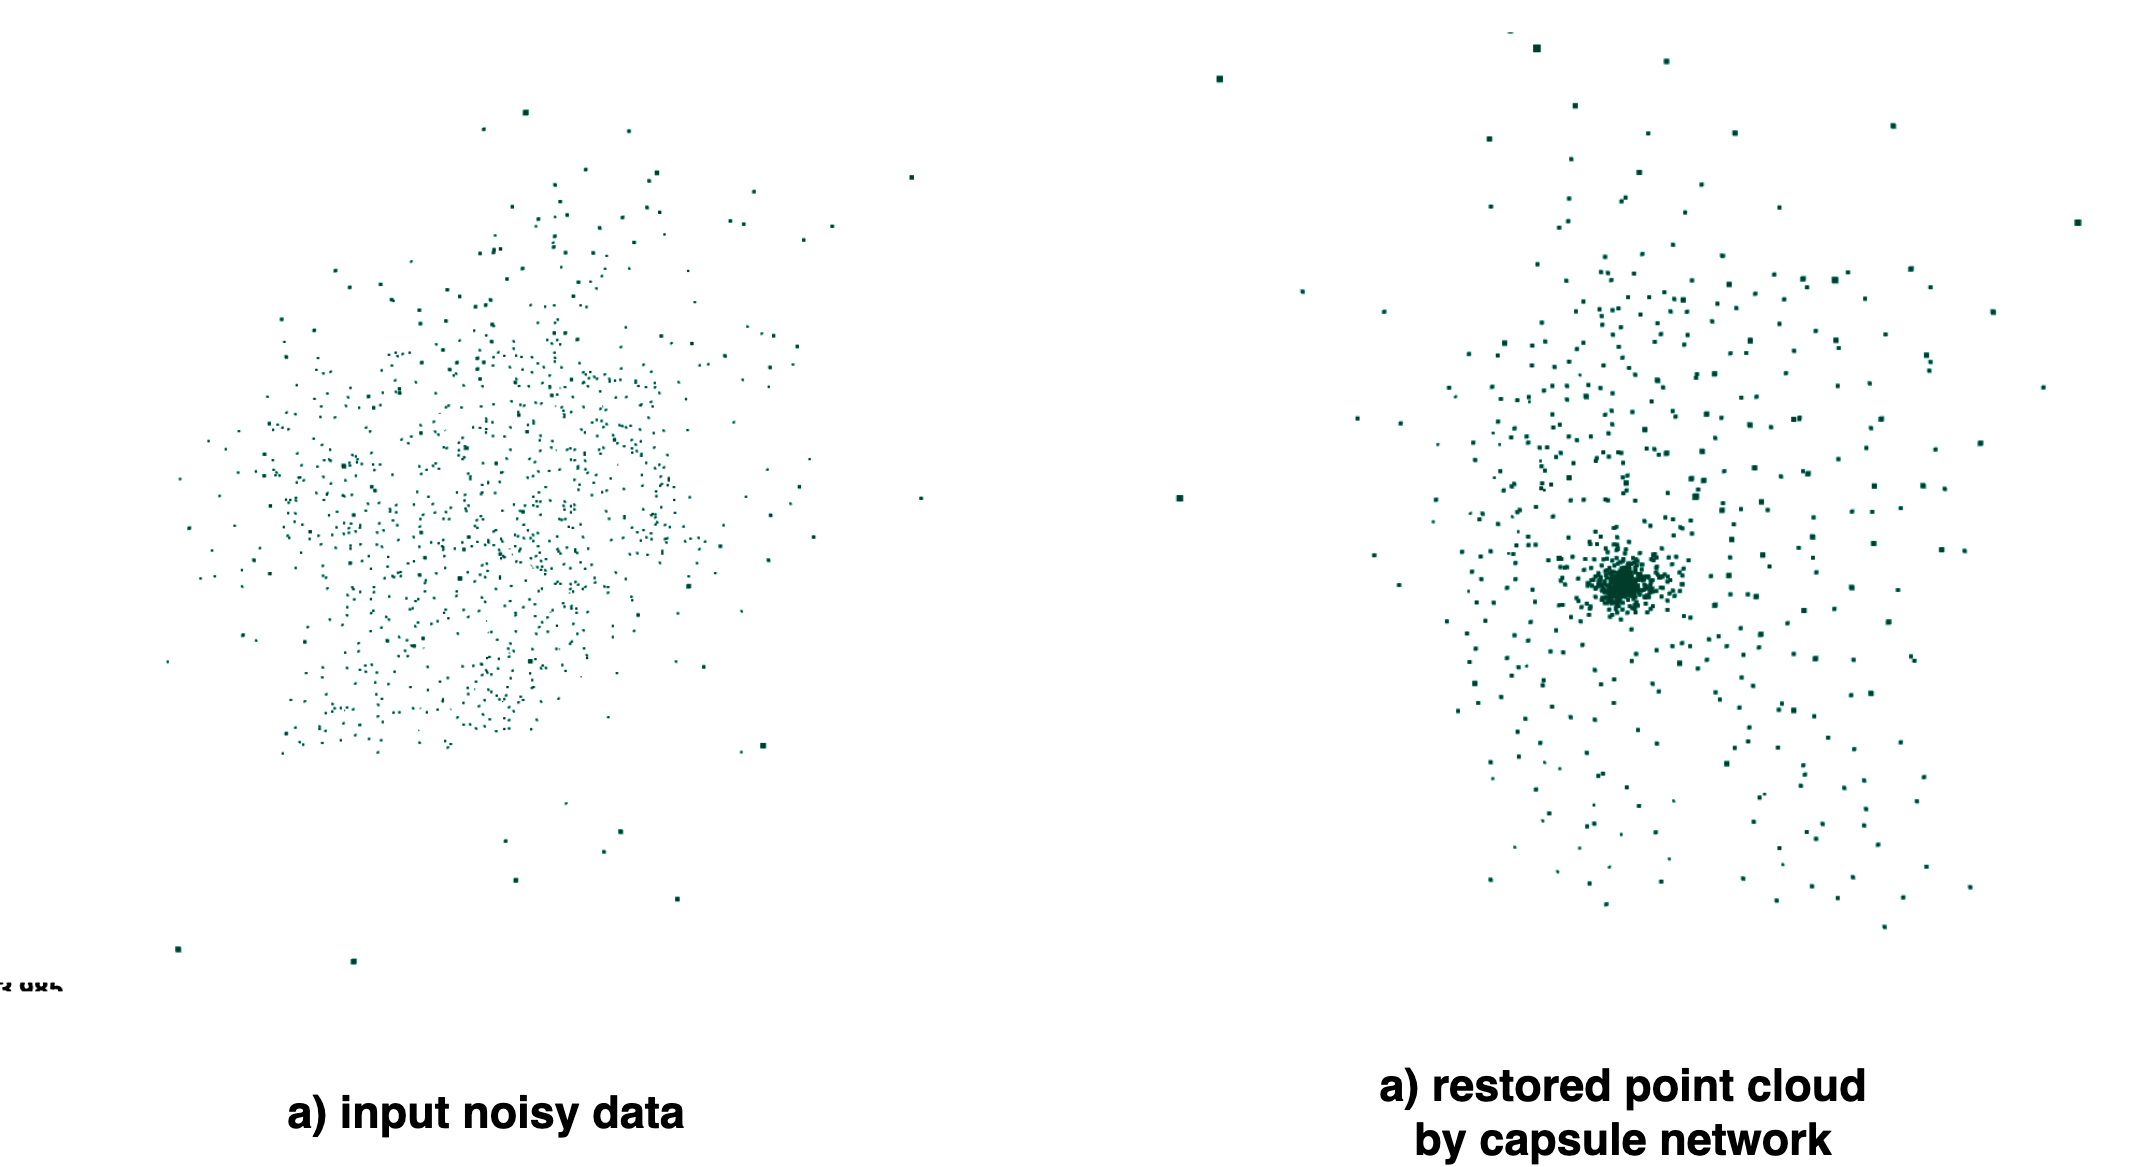
\includegraphics[scale=0.2]{Figures/noise-resporation.png}}
    \caption{Example of noisy point cloud (left), and restored point cloud by capsule network (left)}
    \label{img:denoising}
\end{figure}

Based on the visual analysis we could say that a capsule-based network filters the majority amount of noisy data and potentially could be used as a denoiser.

\section{Models' performance with the lack of data}
\label{s:experiment-lack-of-data}
In this section, we evaluate the capsule-based model with different amounts of training data. Also, we compare the performance with the SOTA model - PoseNet.

For the capsule-based model, we run training pipelines with different training dataset sizes (16/16 as a reference, 15/16, 12/16, and 8/16). The pipeline setup is described in Section~\ref{s:experiment-setup}. After each run of training, we measure the mAP for 10 cm distance on the test dataset.

For PoseNet we use the same approach of retraining the model with different train sizes. The training code was used from the original\footnote{\url{https://github.com/mks0601/V2V-PoseNet_RELEASE}} implementation of the model. Also, we use default parameters for the PoseNet network.

As a benchmark dataset, we use the ITOP side view.

The comparison table for the set of experiments could be found in Table~\ref{tab:truncated-data}.

\begin{table}[H]
    \caption{The comparison of capsnet model and PoseNet trained on different amound of data (ITOP side view)}
    \label{tab:truncated-data}
    \centering
    \begin{tabular}{l l l l l}
    \toprule
    \tabhead{Dataset size} & \tabhead{PoseNet} & \tabhead{CapsNet} & \tabhead{PoseNet difference} & \tabhead{CapsNet difference}  \\
    \midrule
    $16/16$ (full dataset) & 86.2\%  & 83.1\%  & 0\% & 0\% \\
    $15/16$ & 86.0\%  & 82.8\%  & 0.2\% & 0,3\% \\
    $12/16$ & 80.2\%  & 74.3\%  & 6,0\% & 8,8\% \\
    $8/16$ & 63.7\%  & 56.0\%  & 30,2\% & 27,1\% \\
    \bottomrule\\
    \end{tabular}
\end{table}

As we can see from the results capsule-based model underperform compared to PoseNet model. The only experiment where the capsule-based model shows a better mAP difference is the case with 8/16 of the dataset. In this experiment capsule model shows $27,1\%$ of mAP drop compared to $30,2\%$ in PoseNet.

Taking everything into account we can't prove a hypothesis that a capsule-based network works better in data lack environment compared to another SOTA model. However, this statement is hold only for current experiment setup and could change on other datasets. 
\chapter{Conclusions}

\label{Conclusions}

\section{What was done?}
In this section we sum up our work which was concentrated on main objectives:
\begin{itemize}
  \item Design a capsule-based model for the task of human pose estimation using point cloud data. Compare model's performance with SOTA models
  \item Verify the hypothesis that capsule-based models perform better compared to others on noisy data
  \item Verify the hypothesis that capsule-based models better generalize and need less training data compared to other models
\end{itemize}

Further in the text, we describe our results for each objection.

\subsubsection{Capsule-based model for human pose estimation}
We designed a capsule-based neural network for human pose estimation using point clouds. We took the work \cite{wu_3d_2020} of as a baseline architecture for our problem. We proposed the new method of one-stage training of the model which showed improved performance both in training speed and in the model's accuracy. We compared our model with SOTA models on the well-known dataset. Our proposed network shows competitive results outperforming such architectures as use as a reference such models: RF \parencite{shotton_real-time_2011}, RTW \parencite{ho_yub_jung_random_2015}, IEF \parencite{carreira_human_2016}, and VI \parencite{haque_towards_2016}. But still our proposed model underperform in comparison with  REN \parencite{chen_pose_2020} and Pose-net \parencite{moon_v2v-posenet_2018} models.

\subsubsection{Capsule-based model and noisy data}
We designed a methodology and conducted experiments to verify the hypothesis that capsule-based networks are more noise agnostic in comparison with non-capsule-based models.

We have evaluated our proposed models and the SOTA PoseNet model on the ITOP dataset with different amounts of artificial noise (from Gaussian and uniform distributions). Based on our experiments capsule-based model shows better results in most of the cases in comparison with PoseNet. Also, we have visually proved that a capsule-based model could denoise the point cloud which we associate with the ability of the capsule network to hold internal representation.

\subsubsection{Capsule-based model and train dataset size}
We designed a methodology and conducted experiments to verify the hypothesis that capsule-based networks need fewer data to train in comparison with non-capsule-based models.

We have evaluated the capsule-based model and SOTA PoseNet model on the ITOP dataset. We have conducted multiple experiments where we reduce the training dataset size. Based on our results we don't see any proofs that capsule-based models could better generalize the data and thus need less training data.

\section{Future work}
Algorithms on point clouds are a really promising field. Capsule-based networks are interesting models for this particular task. Capsule-based models could hold an internal representation of the input data and thus reuse it to improve performance for a variety of tasks like classification, segmentation, regression, etc.

We have shown that capsule-based models are applicable for the task of human pose estimation, and could show compatible results.

As future work we see such areas:

\subsubsection{Data preprocessing}
We proposed a method where we preprocess the initial point cloud and extract a person point cloud, and only then use it as an input to the network. Such an approach is not applicable to the real-world data since our techniques are greatly tight to the ITOP dataset.

To better adapt a pipeline to the real-world use case the special extraction DNN models could be used \parencite{shi_points_2020,yang_pixor_2019}. Such models don't need handcrafted thresholds and parameters thus could be used for more diverse datasets.

\subsubsection{New datasets}
Our research was focused on the ITOP dataset. But the EVAL dataset mentioned in Section-\ref{Dataset} also could be used for the evaluation. 

\subsubsection{New loss aggregation strategies}
In our work, we use the product of losses as an aggregation strategy. Also, we use the logarithm to mitigate the issue of vanishing gradient. This approach is quite primitive and some advanced loss aggregations methods could be used \parencite{noauthor_optimizing_nodate}. 

%----------------------------------------------------------------------------------------
%	THESIS CONTENT - APPENDICES
%----------------------------------------------------------------------------------------

\appendix % Cue to tell LaTeX that the following "chapters" are Appendices

% Include the appendices of the thesis as separate files from the Appendices folder
% Uncomment the lines as you write the Appendices

% % Appendix A

\chapter{Frequently Asked Questions} % Main appendix title

\label{AppendixA} % For referencing this appendix elsewhere, use \ref{AppendixA}

\section{How do I change the colors of links?}

The color of links can be changed to your liking using:

{\small\verb!\hypersetup{urlcolor=red}!}, or

{\small\verb!\hypersetup{citecolor=green}!}, or

{\small\verb!\hypersetup{allcolor=blue}!}.

\noindent If you want to completely hide the links, you can use:

{\small\verb!\hypersetup{allcolors=.}!}, or even better: 

{\small\verb!\hypersetup{hidelinks}!}.

\noindent If you want to have obvious links in the PDF but not the printed text, use:

{\small\verb!\hypersetup{colorlinks=false}!}.

%\include{Appendices/AppendixB}
%\include{Appendices/AppendixC}

%----------------------------------------------------------------------------------------
%	BIBLIOGRAPHY
%----------------------------------------------------------------------------------------

\printbibliography[heading=bibintoc]

%----------------------------------------------------------------------------------------

\end{document}  
